\documentclass{beamer}
\usepackage[utf8]{inputenc}
\usepackage[spanish]{babel}
\usepackage{graphicx}
\usepackage{booktabs}
\usepackage{ragged2e}
\usepackage{xcolor}
\definecolor{LightGray}{gray}{0.975}
\definecolor{links}{HTML}{2A1B81}
\hypersetup{colorlinks,linkcolor=,urlcolor=blue}

\usepackage{tikz}
\usetikzlibrary{arrows,shapes}

\usepackage{algorithm}
\usepackage{algorithmic}

%\usepackage{minted}
\usepackage{xcolor}
\definecolor{LightGray}{gray}{0.975}

%\usetheme{Warsaw}
\usefonttheme{serif}

\newcommand\Wider[2][18mm]{%
    \makebox[\linewidth][c]{%
        \begin{minipage}{\dimexpr\textwidth+#1\relax}
            \raggedright#2
        \end{minipage}%
    }%
}

\title[Data Analytics]{Database Administration}
\subtitle{Lecture 10: Data Analytics.}
\author{Silberschatz, Korth \& Sudarshan}
\date{\today}

\setbeamertemplate{navigation symbols}{}%remove navigation symbols

\defbeamertemplate*{footline}{shadow theme}{%
    \leavevmode%
    \hbox{
        \begin{beamercolorbox}[wd=.5\paperwidth,ht=2.5ex,dp=1.125ex,leftskip=.3cm plus1fil,rightskip=.3cm]{author in head/foot}%
            \usebeamerfont{
                author in head/foot
            } Database Administration \hfill \insertshorttitle
        \end{beamercolorbox}%
        \begin{beamercolorbox}[wd=.5\paperwidth,ht=2.5ex,dp=1.125ex,leftskip=.3cm,rightskip=.3cm plus1fil]{title in head/foot}%
            \usebeamerfont{
                title in head/foot
            } \hfill \insertframenumber\,/\,\inserttotalframenumber
        \end{beamercolorbox}
    }
}

\AtBeginSection[]{
    \begin{frame}<beamer>
        \frametitle{Plan}
        \tableofcontents[currentsection]
    \end{frame}
}

\newcommand{\toRight}[1]{
    \begin{FlushRight}
        {\tiny #1}
    \end{FlushRight}
}

\begin{document}

\frame{\titlepage}

\begin{frame}{Database Administration: Data Analytics.}
    \centering
    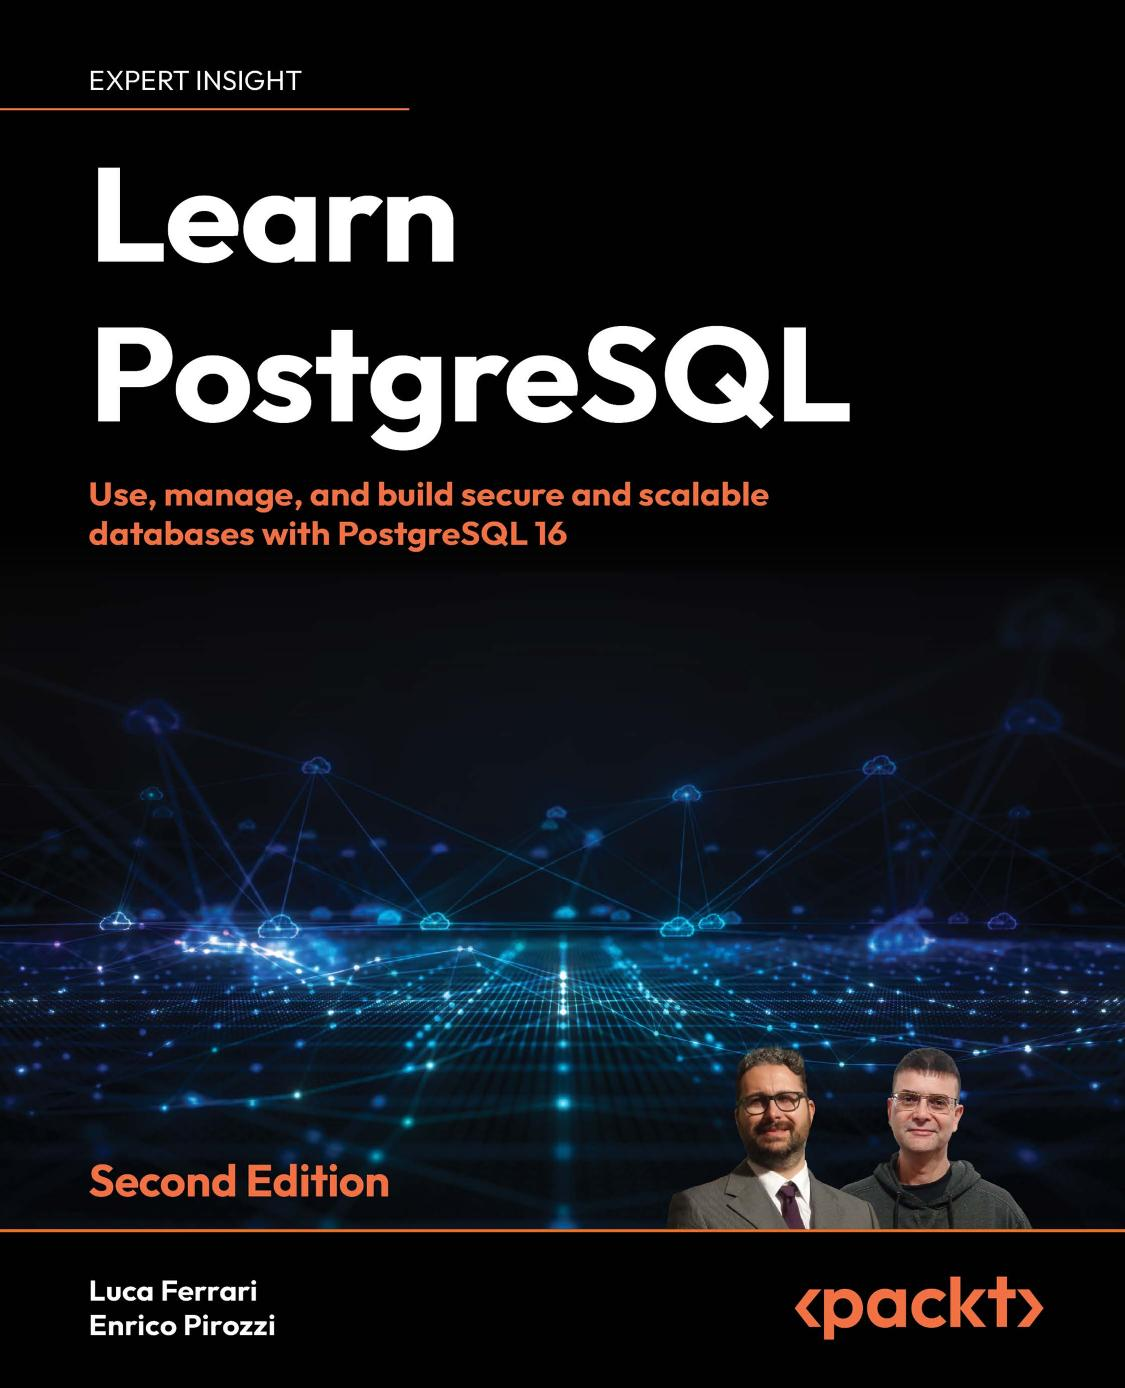
\includegraphics[width=0.4\textwidth]{figures/book_cover}\\
    \vspace{2mm}
    {
        \scriptsize
        Content has been extracted from \textit{Database System Concepts 7ed (Chapter 11)}, by Abraham Silberschatz, Henry Korth \& S. Sudarshan, 2019.  Visit \url{https://db-book.com/}.
    }
\end{frame}

\section{Overview}

\begin{frame}{}
    \Wider{ 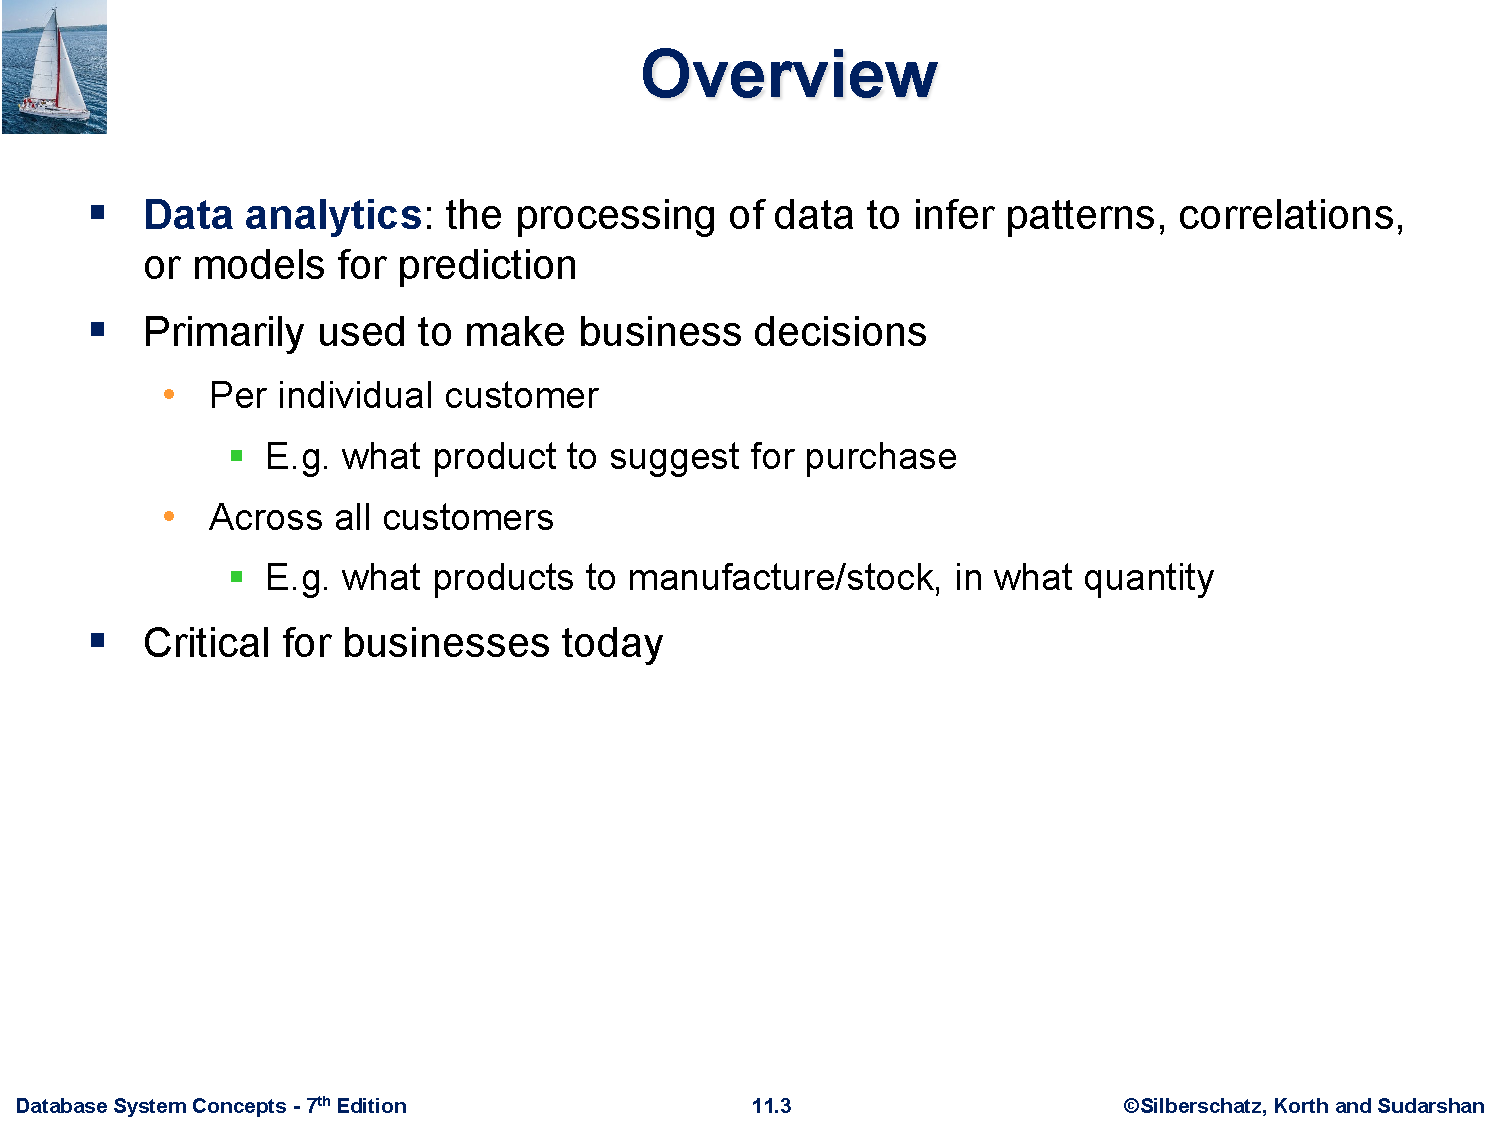
\includegraphics[width=\textwidth, trim={0cm 1cm 0cm 0cm}, clip]{slides/s3} }
\end{frame}
\begin{frame}{}
    \Wider{ 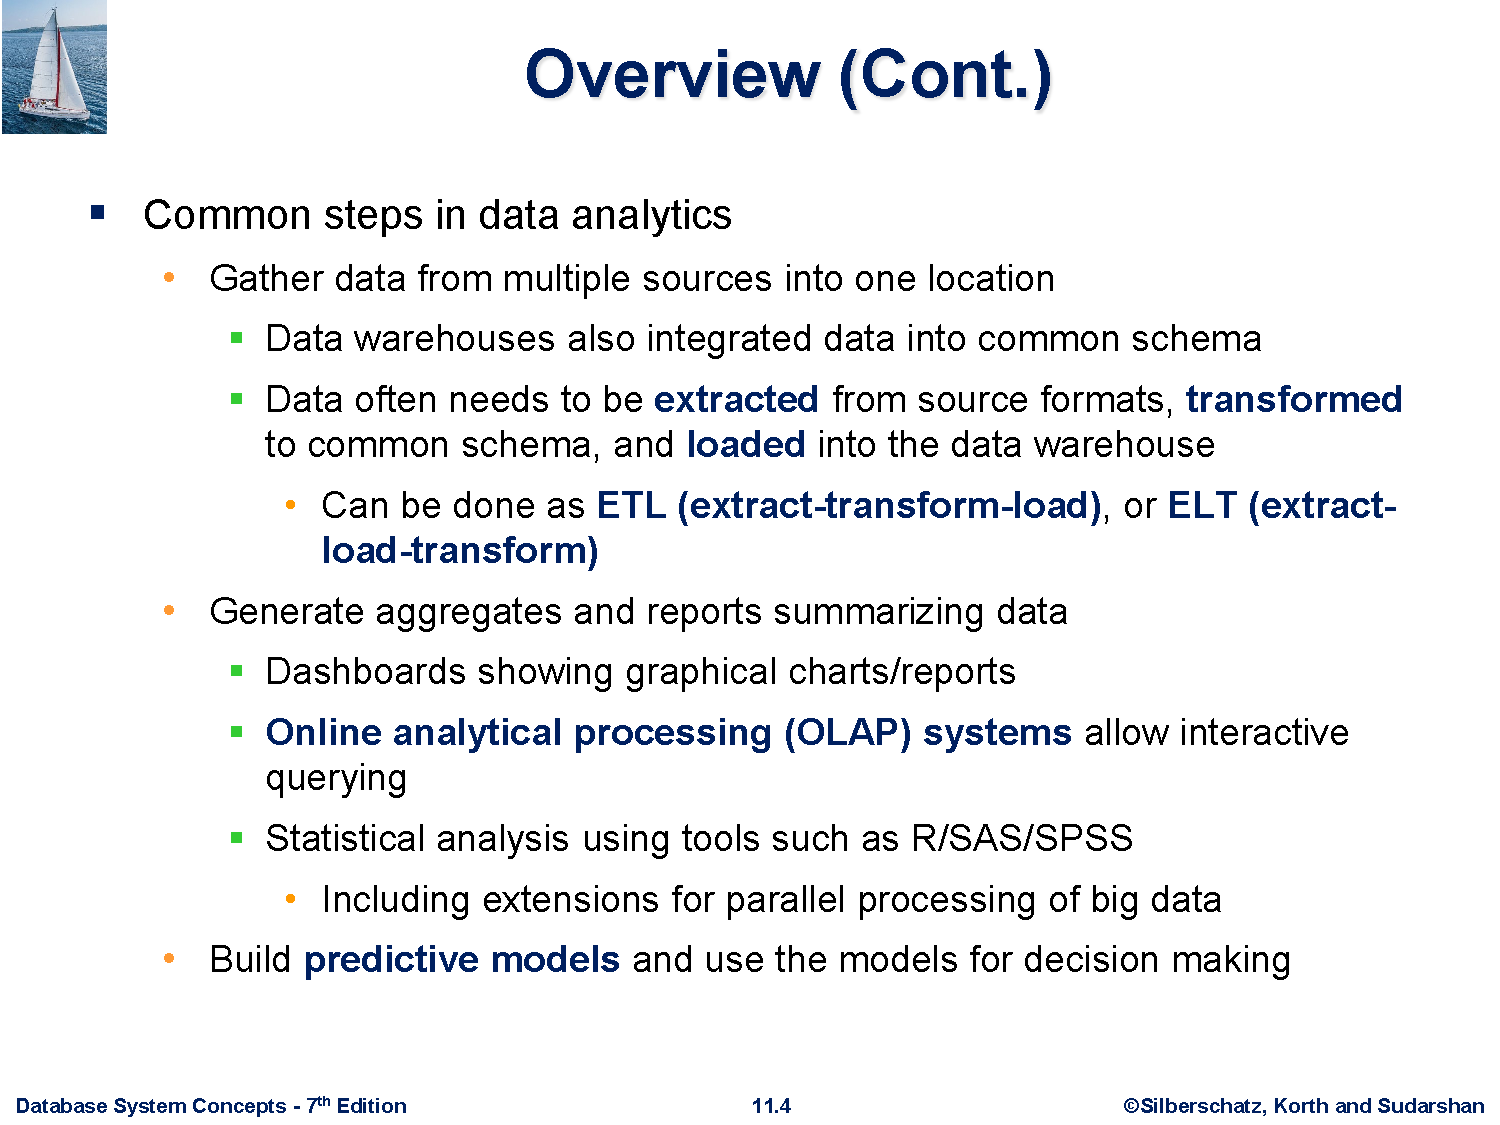
\includegraphics[width=\textwidth, trim={0cm 1cm 0cm 0cm}, clip]{slides/s4} }
\end{frame}
\begin{frame}{}
    \Wider{ 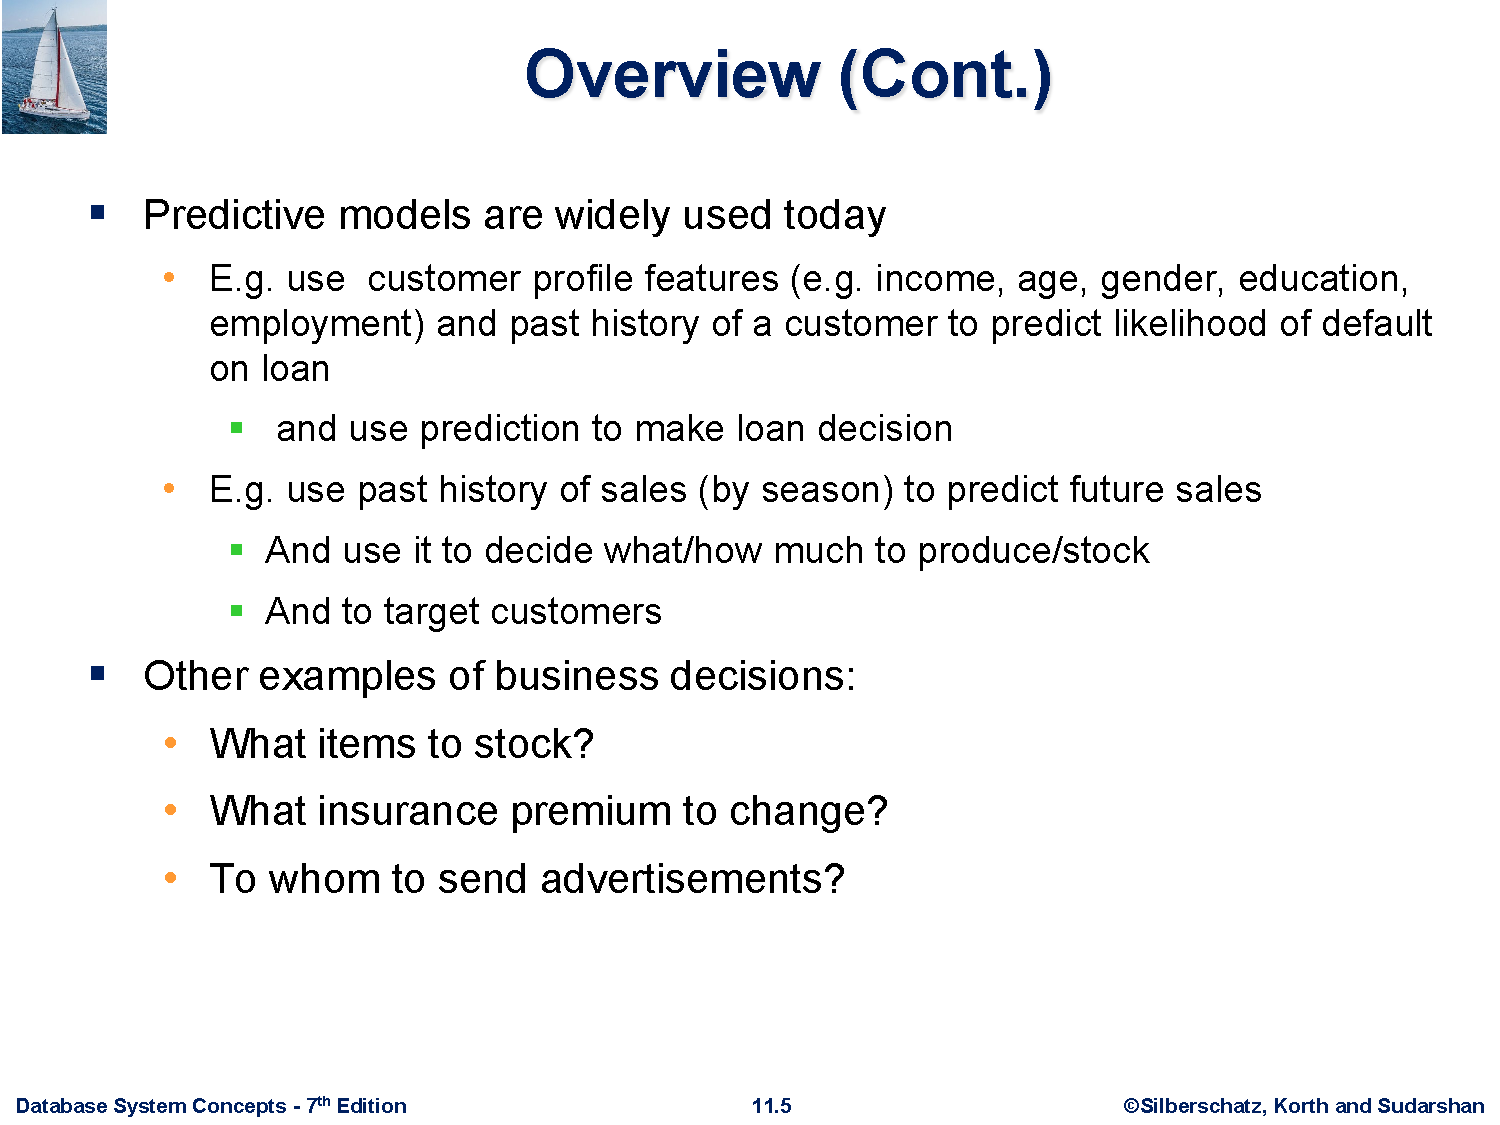
\includegraphics[width=\textwidth, trim={0cm 1cm 0cm 0cm}, clip]{slides/s5} }
\end{frame}
\begin{frame}{}
    \Wider{ 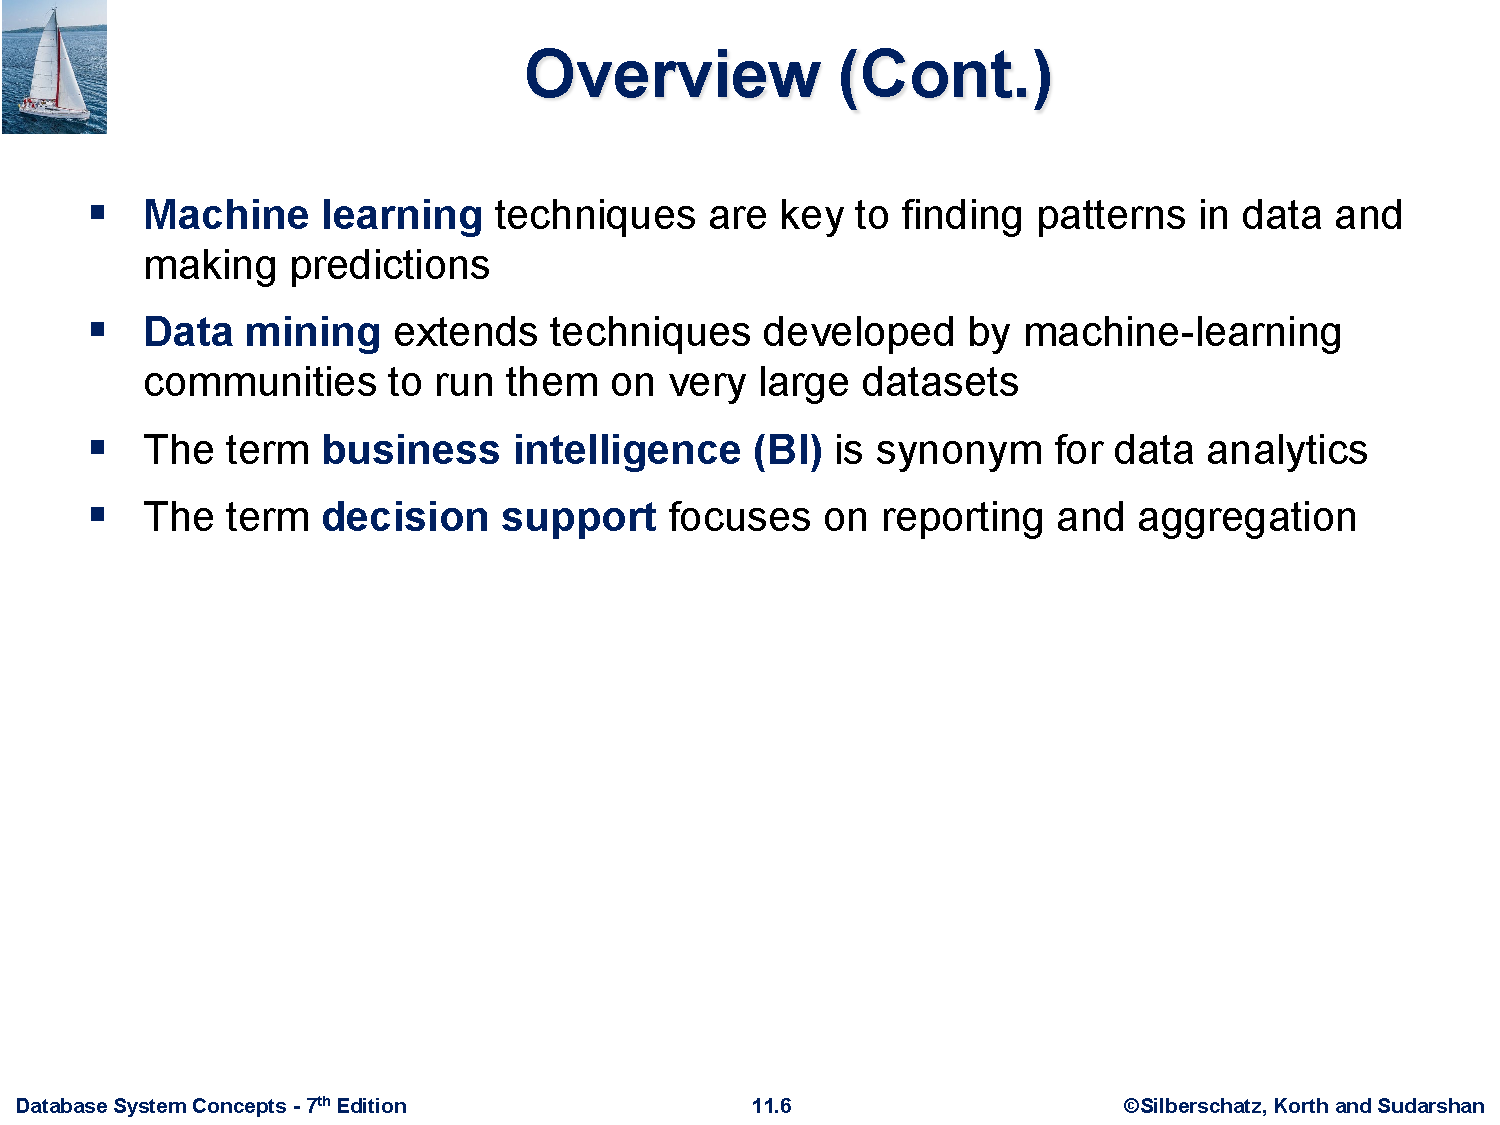
\includegraphics[width=\textwidth, trim={0cm 1cm 0cm 0cm}, clip]{slides/s6} }
\end{frame}

\section{Data Warehousing}

\begin{frame}{}
    \Wider{ 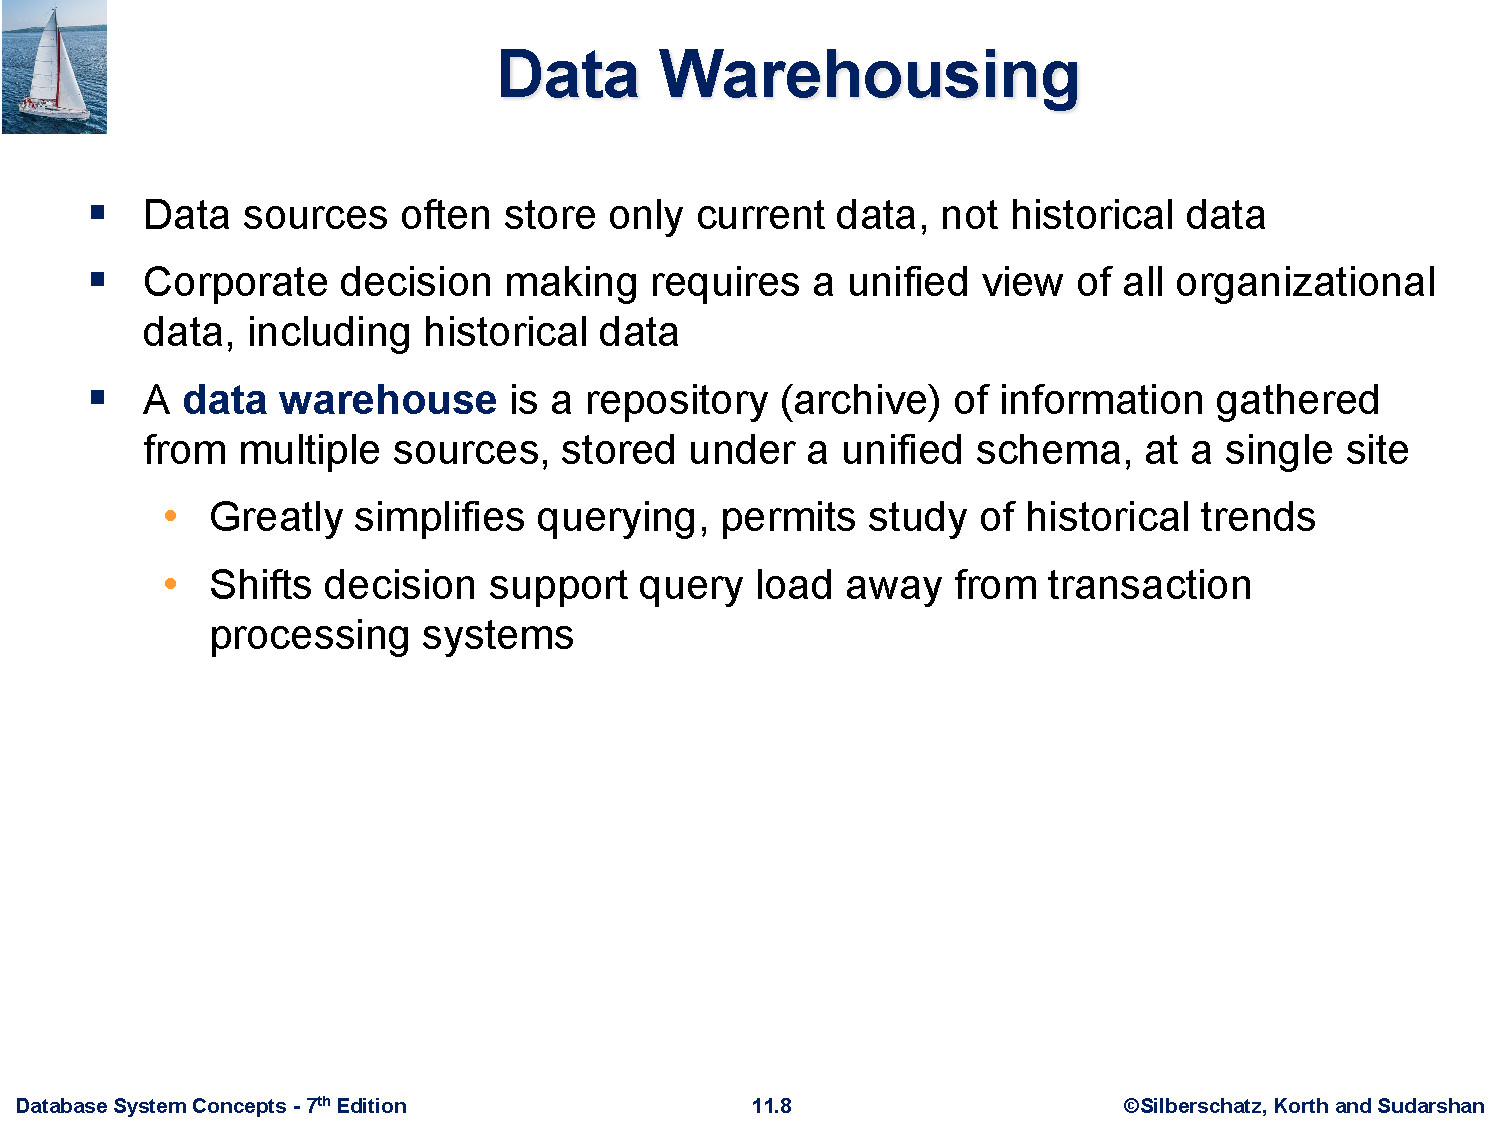
\includegraphics[width=\textwidth, trim={0cm 1cm 0cm 0cm}, clip]{slides/s8} }
\end{frame}
\begin{frame}{}
    \Wider{ 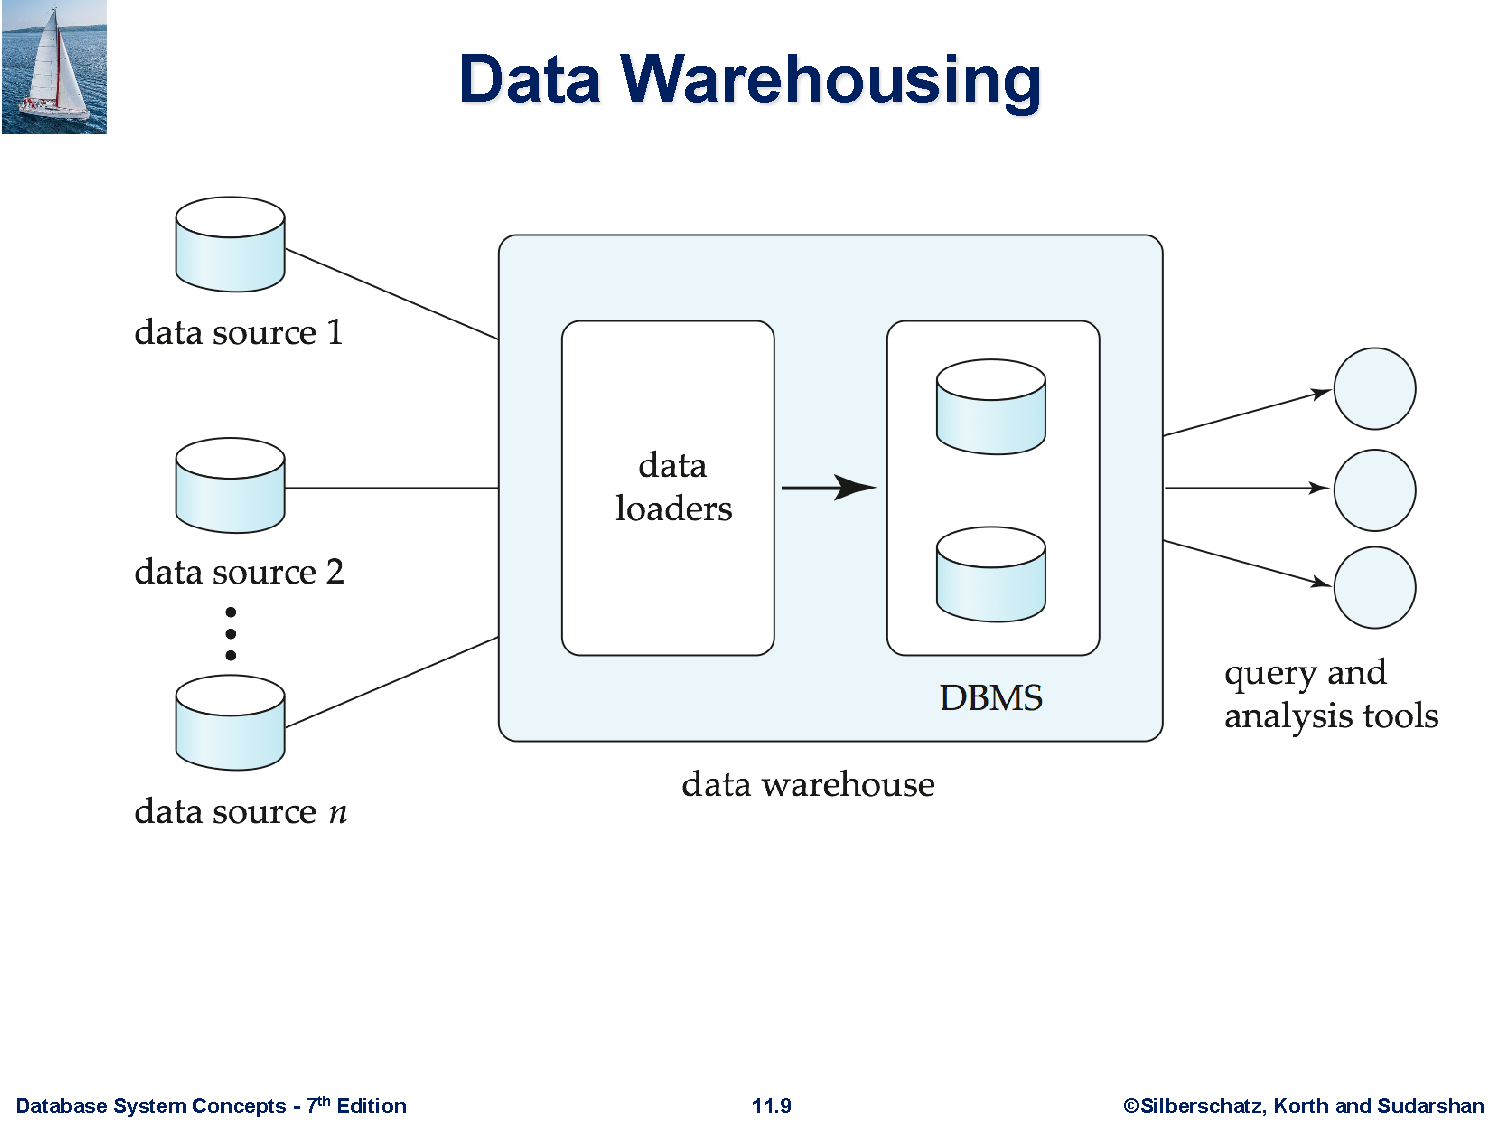
\includegraphics[width=\textwidth, trim={0cm 1cm 0cm 0cm}, clip]{slides/s9} }
\end{frame}
\begin{frame}{}
    \Wider{ 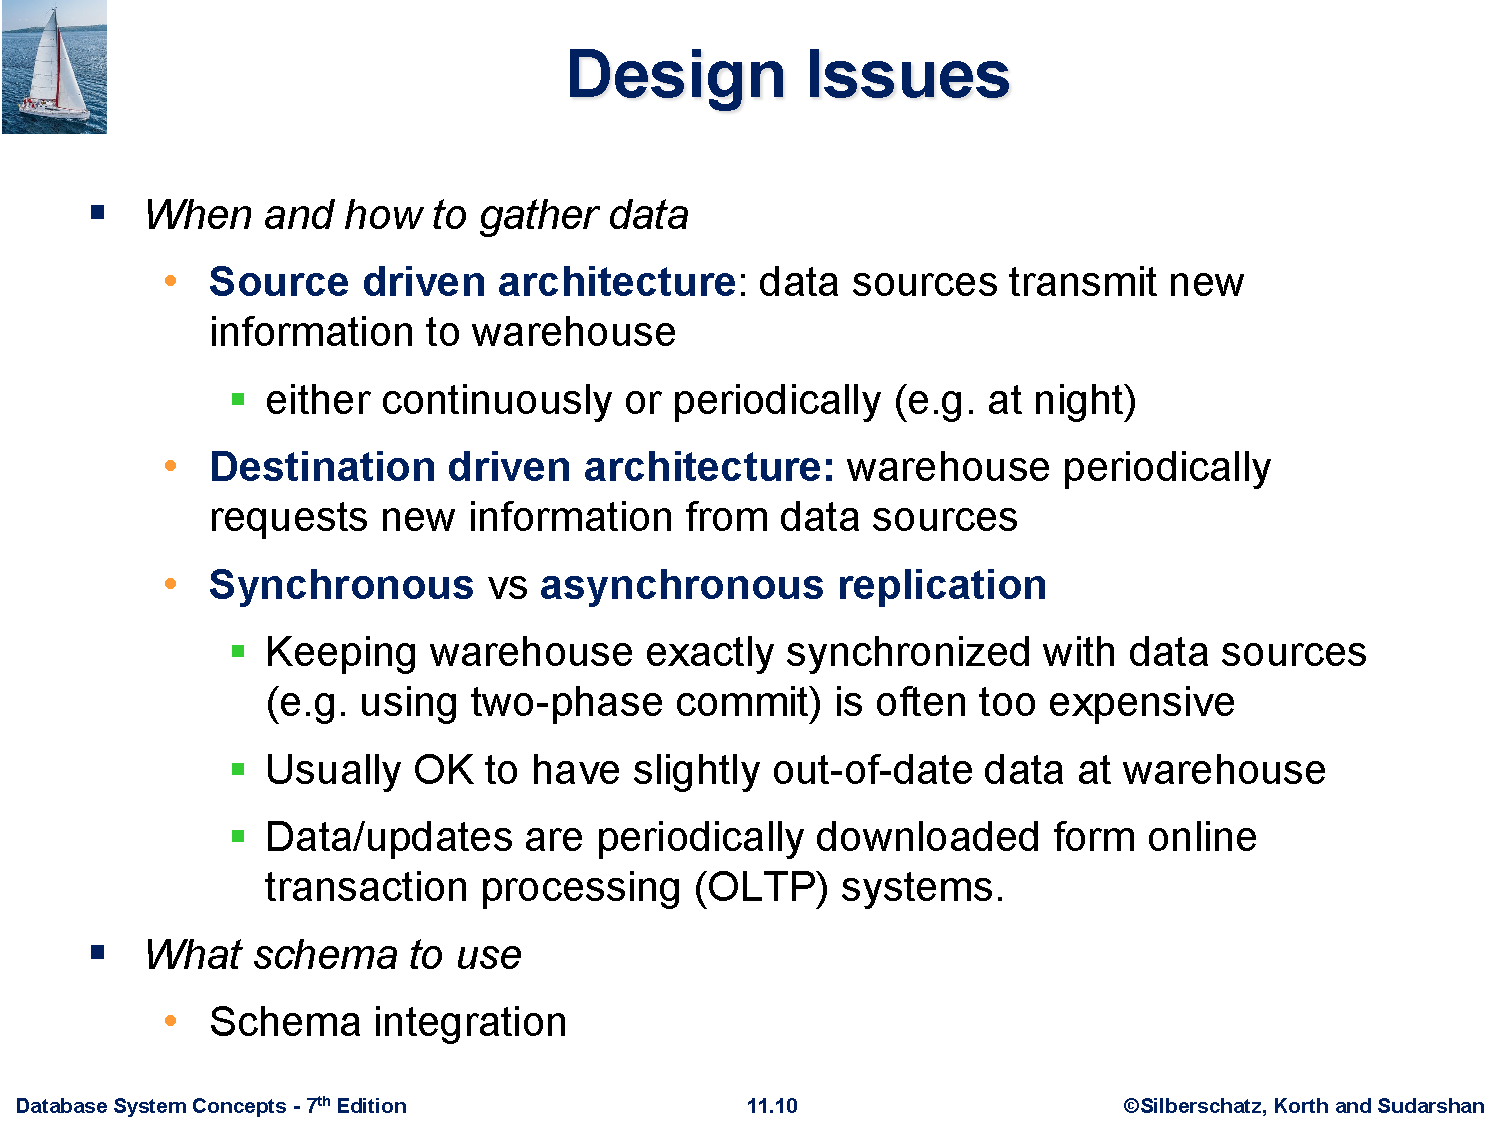
\includegraphics[width=\textwidth, trim={0cm 1cm 0cm 0cm}, clip]{slides/s10} }
\end{frame}
\begin{frame}{}
    \Wider{ 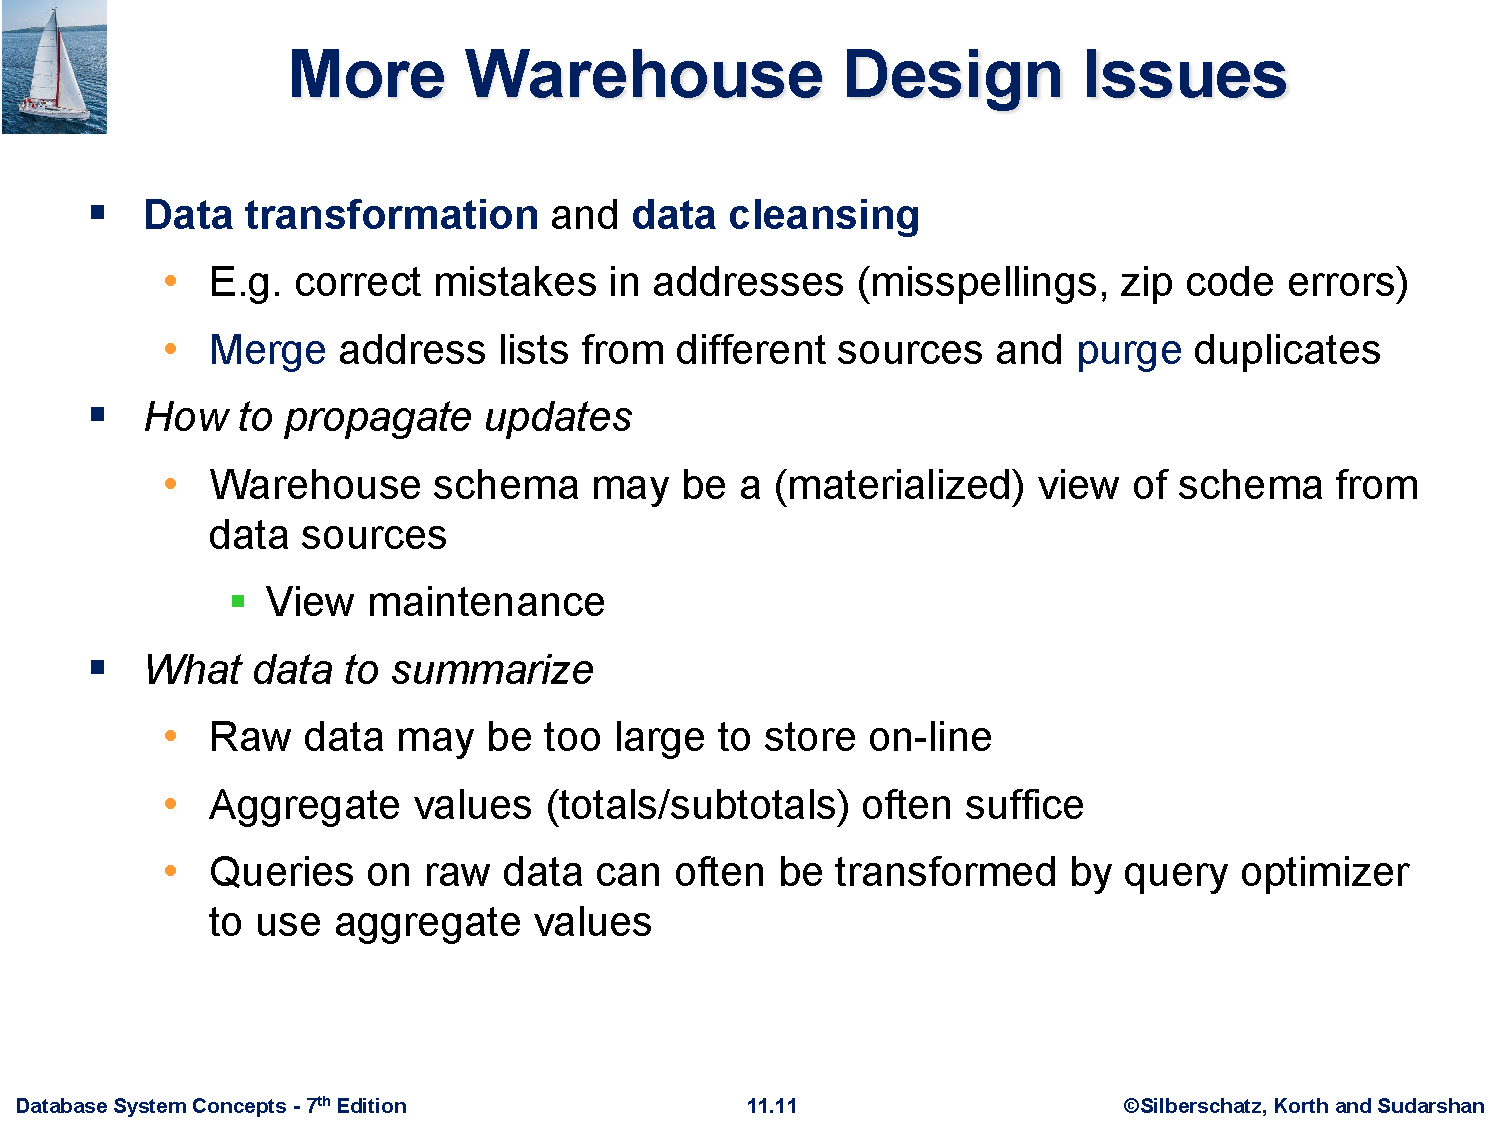
\includegraphics[width=\textwidth, trim={0cm 1cm 0cm 0cm}, clip]{slides/s11} }
\end{frame}
\begin{frame}{}
    \Wider{ 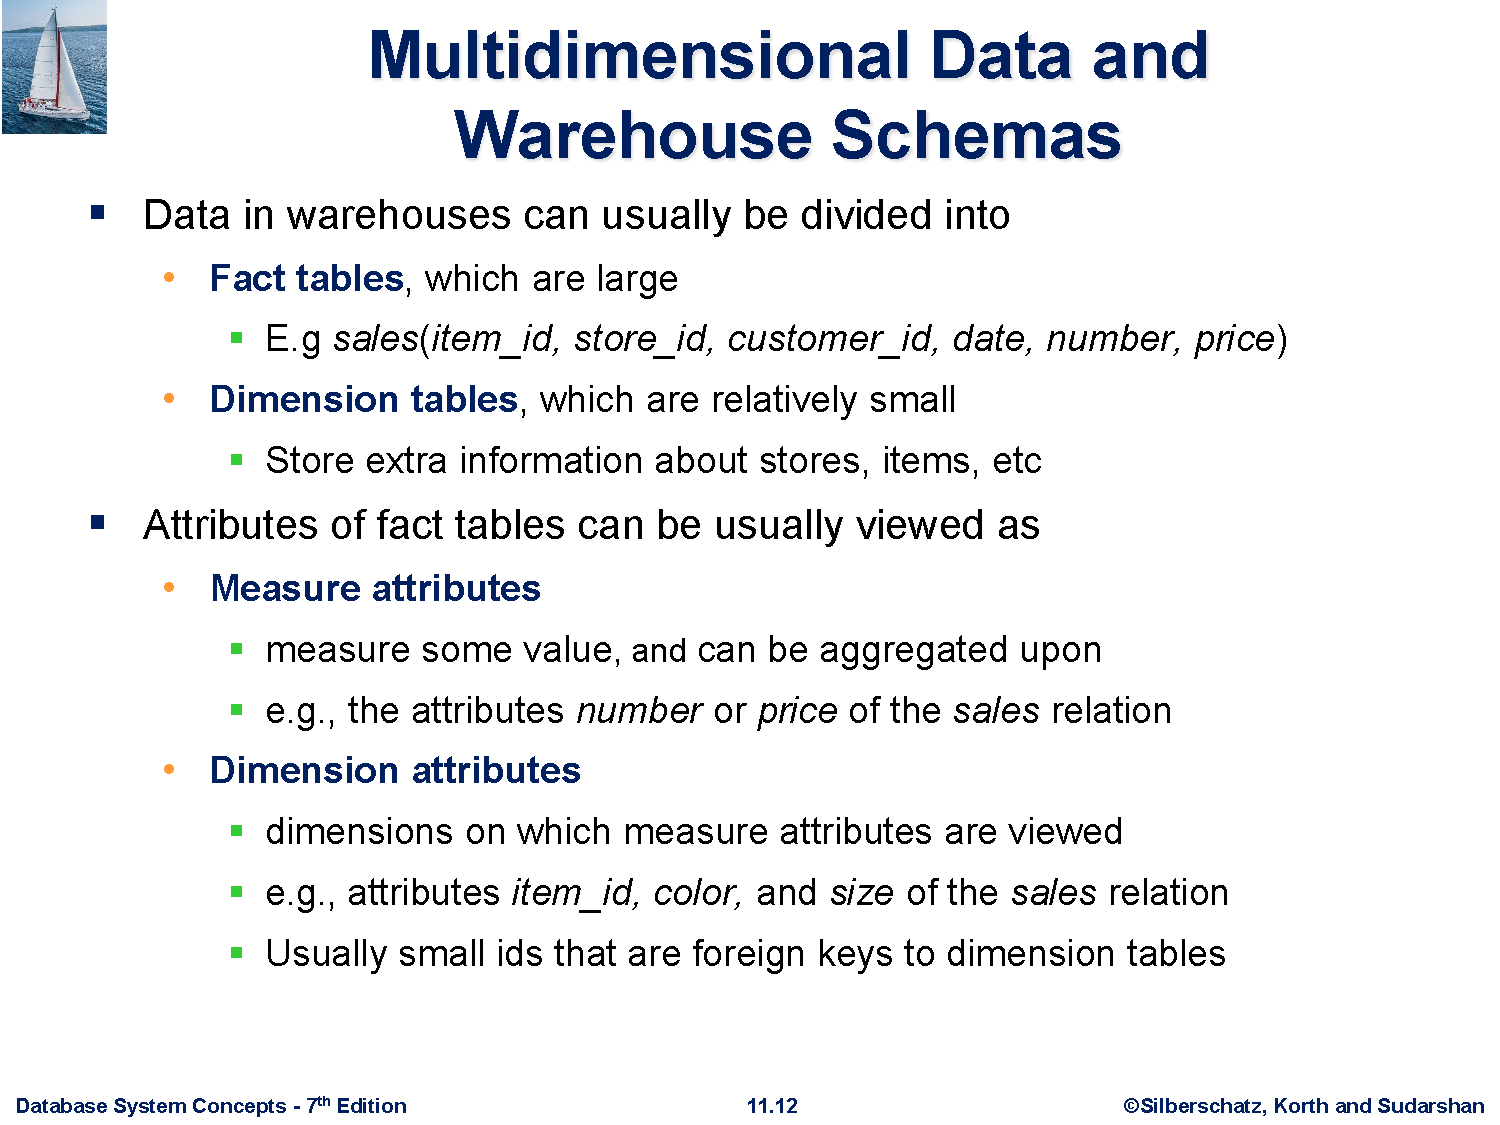
\includegraphics[width=\textwidth, trim={0cm 1cm 0cm 0cm}, clip]{slides/s12} }
\end{frame}
\begin{frame}{}
    \Wider{ 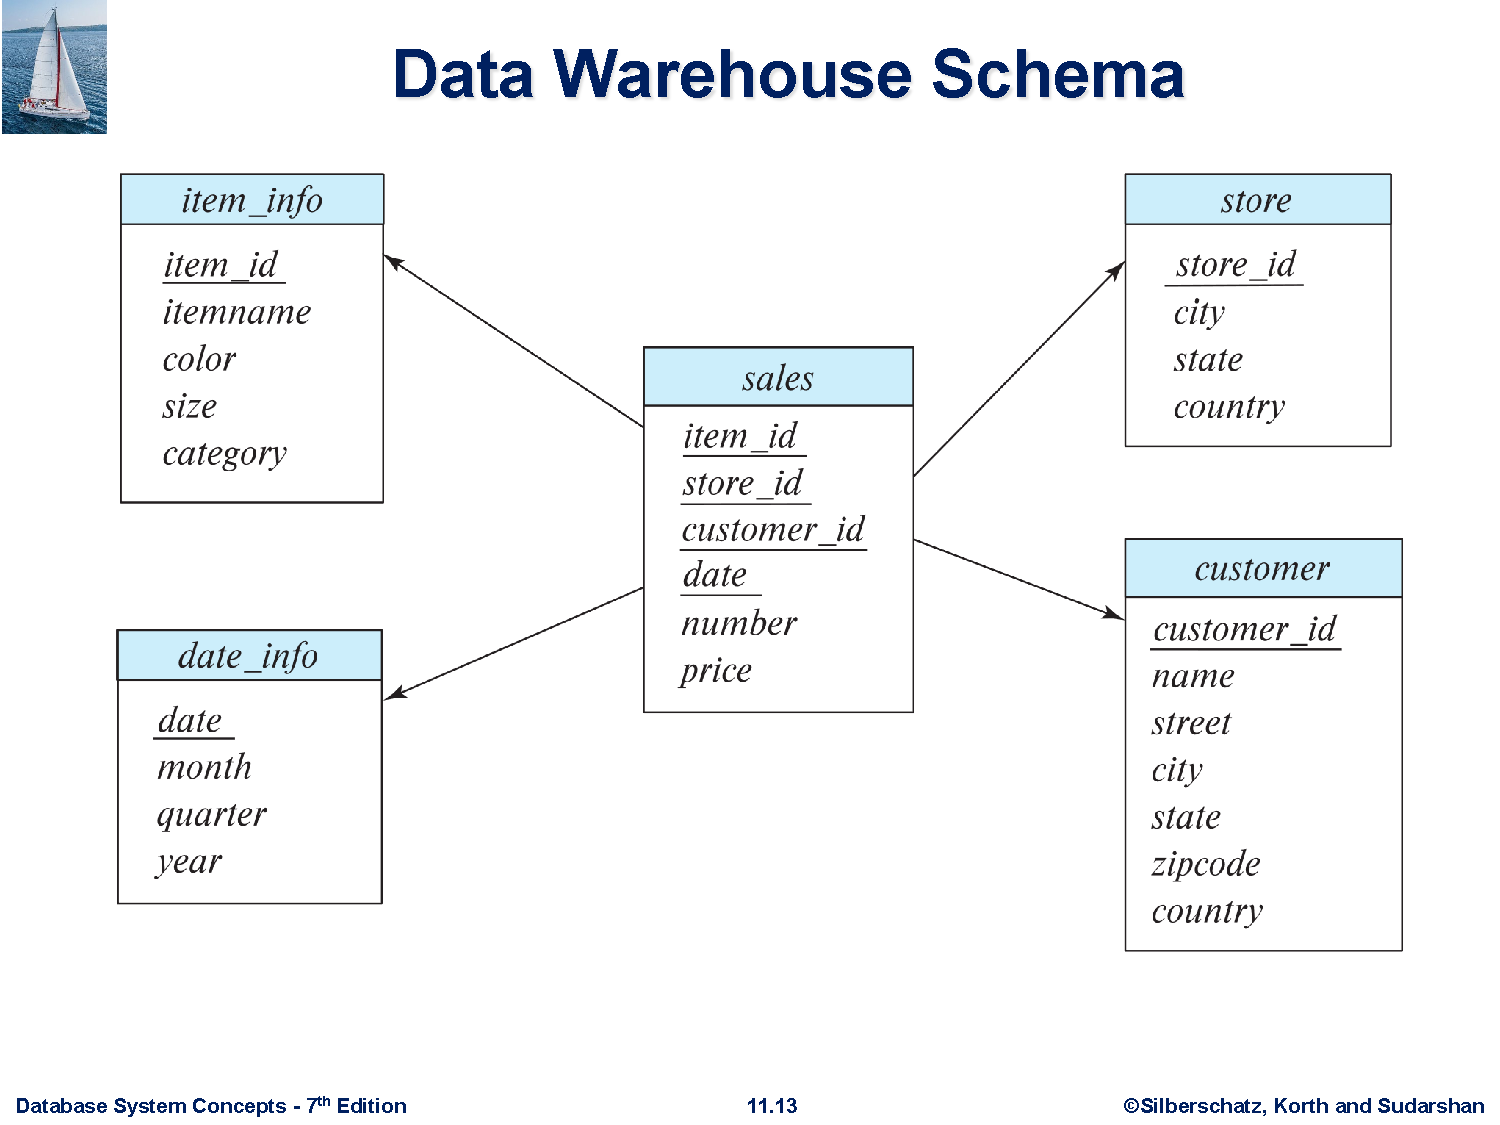
\includegraphics[width=\textwidth, trim={0cm 1cm 0cm 0cm}, clip]{slides/s13} }
\end{frame}
\begin{frame}{}
    \Wider{ 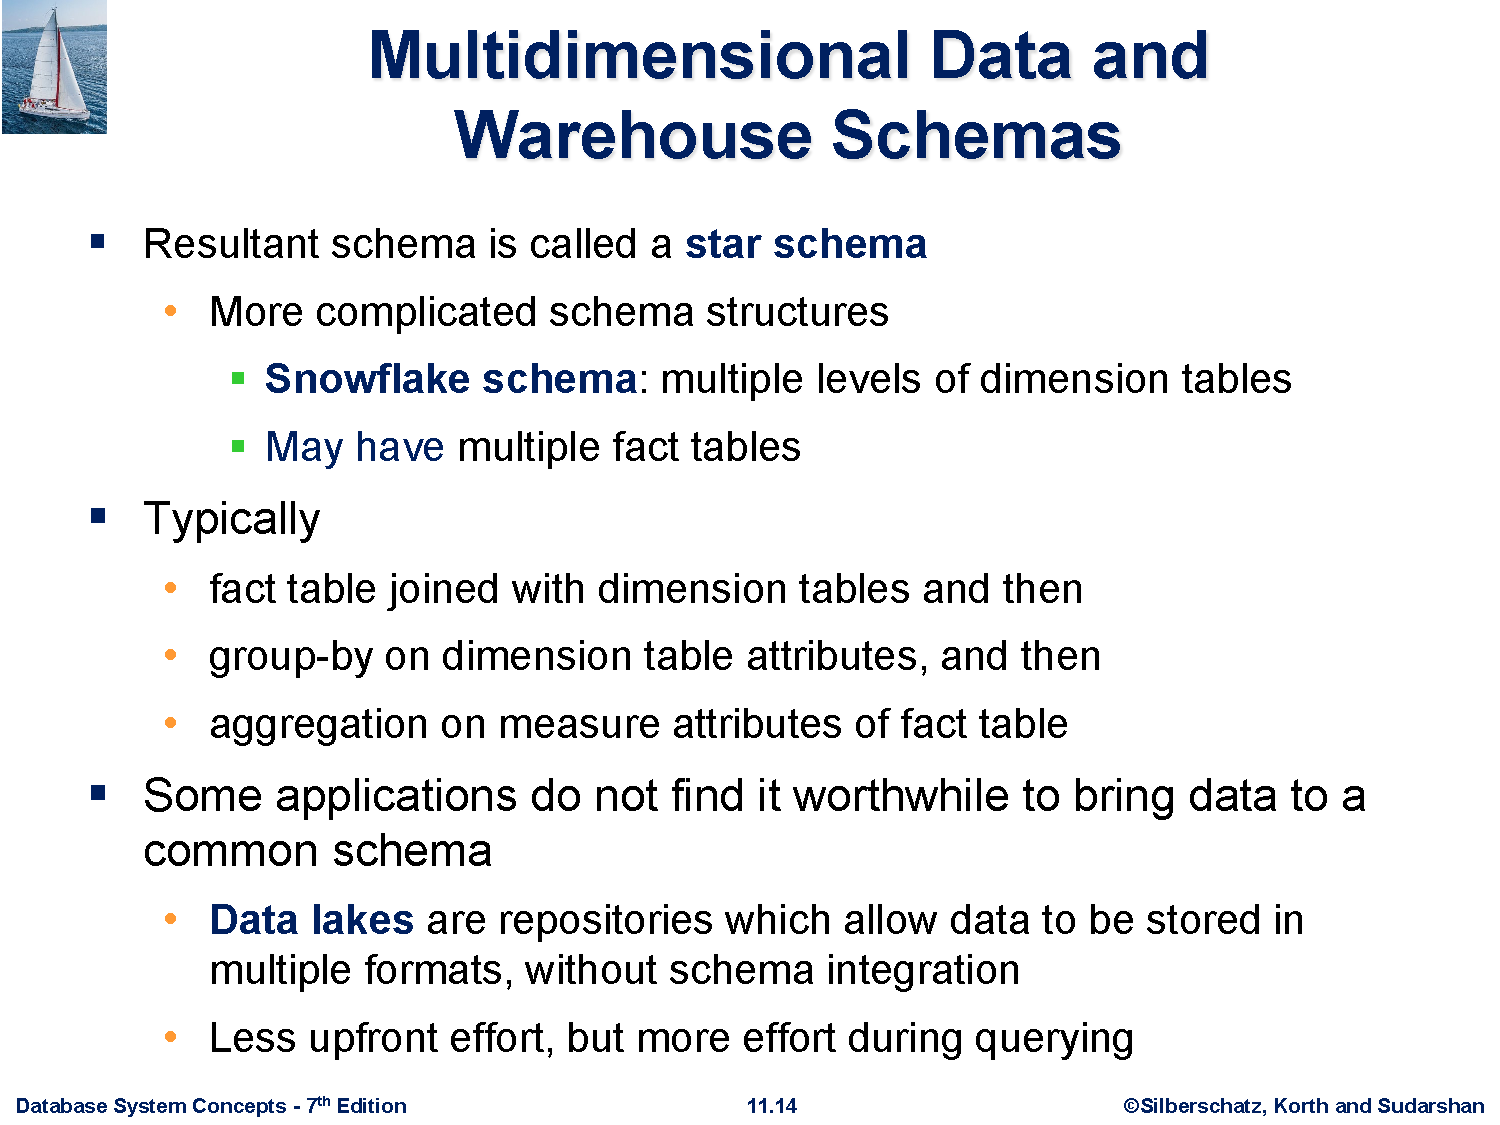
\includegraphics[width=\textwidth, trim={0cm 1cm 0cm 0cm}, clip]{slides/s14} }
\end{frame}
\begin{frame}{}
    \Wider{ 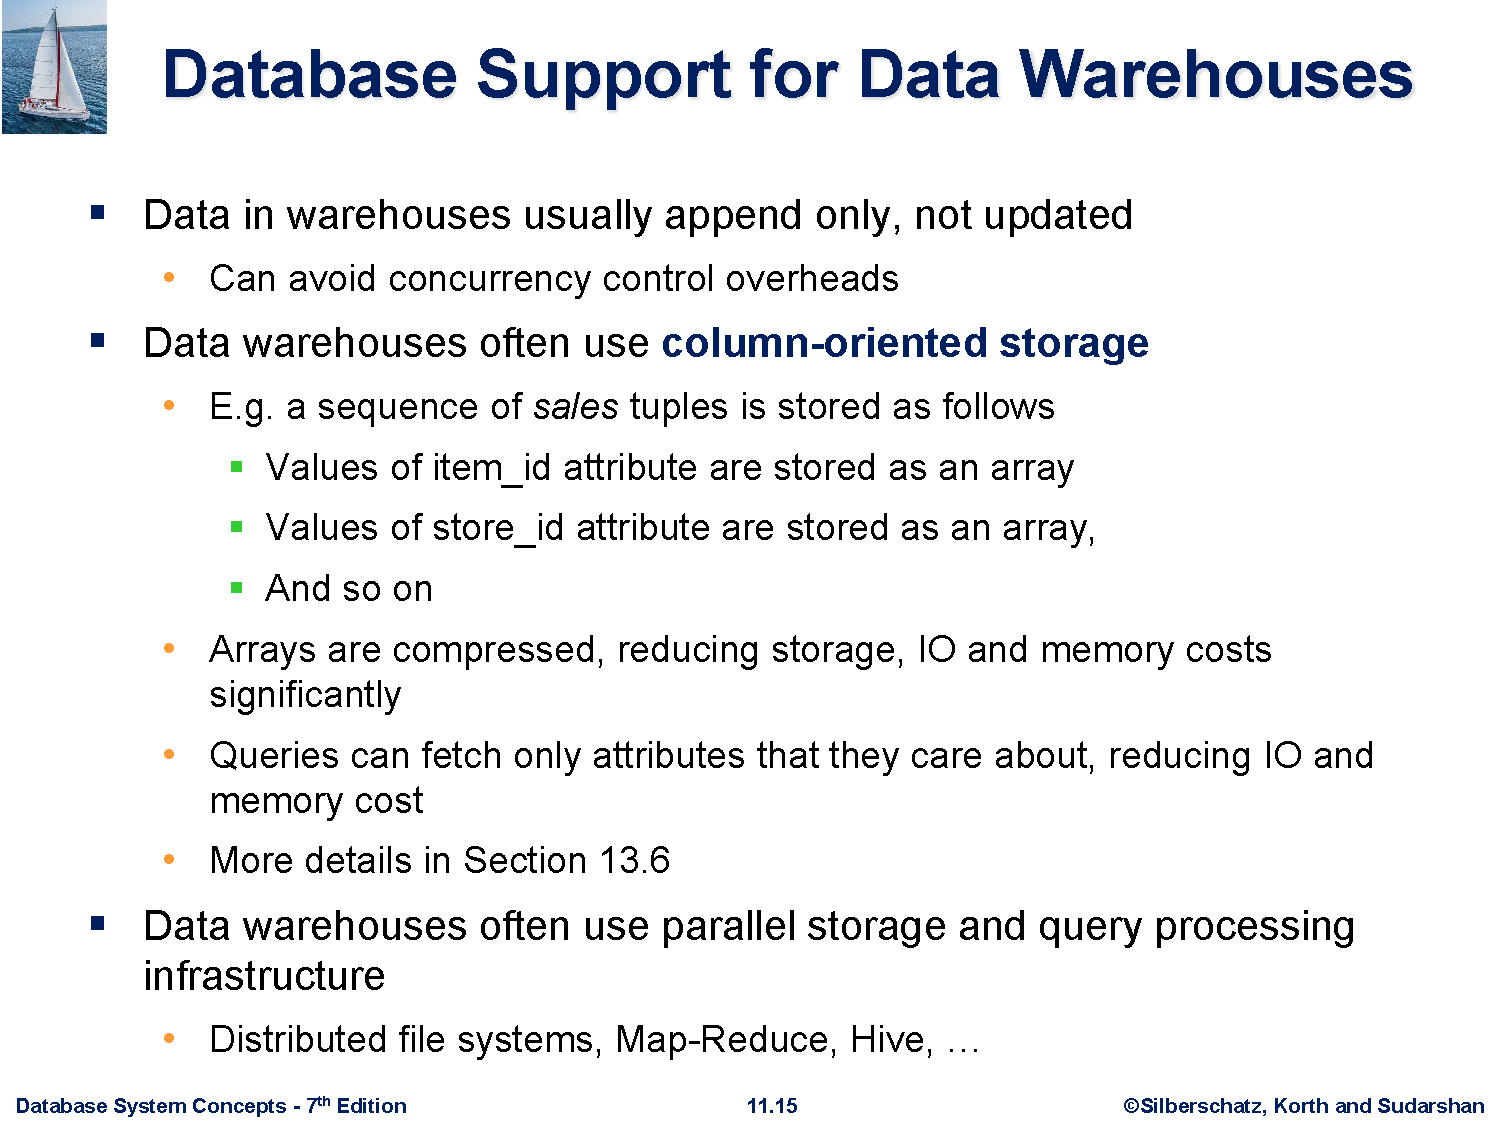
\includegraphics[width=\textwidth, trim={0cm 1cm 0cm 0cm}, clip]{slides/s15} }
\end{frame}

\section{OLAP}

\begin{frame}{}
    \Wider{ 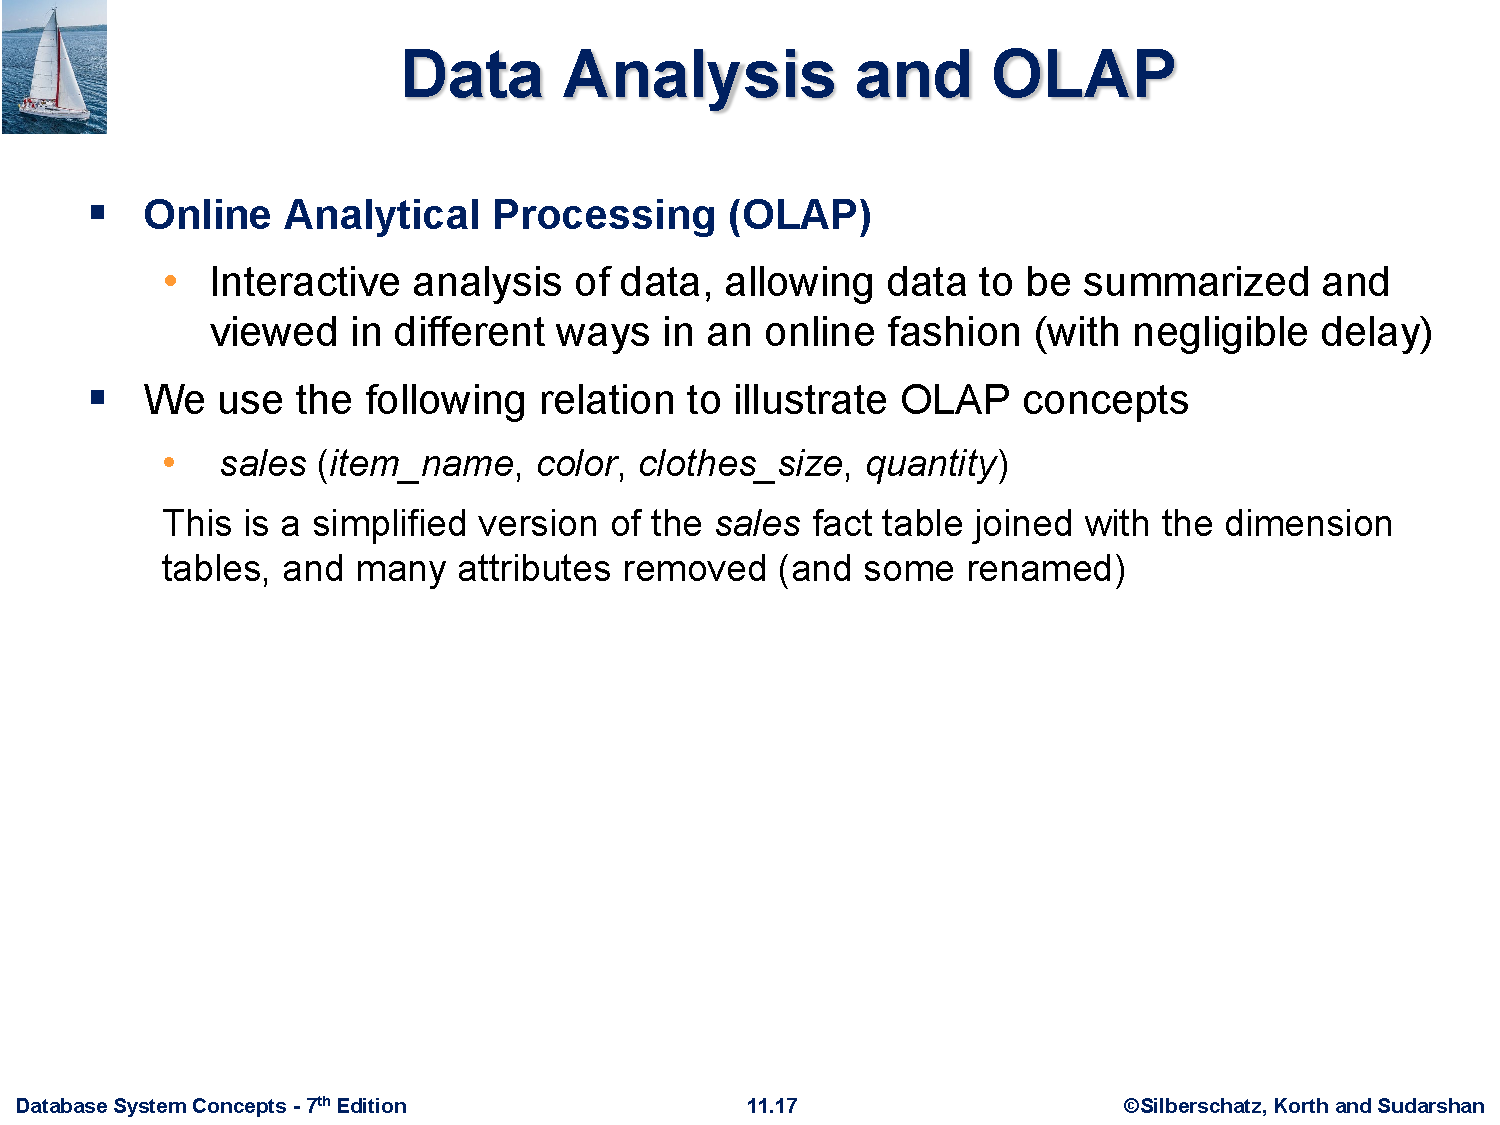
\includegraphics[width=\textwidth, trim={0cm 1cm 0cm 0cm}, clip]{slides/s17} }
\end{frame}
\begin{frame}{}
    \Wider{ 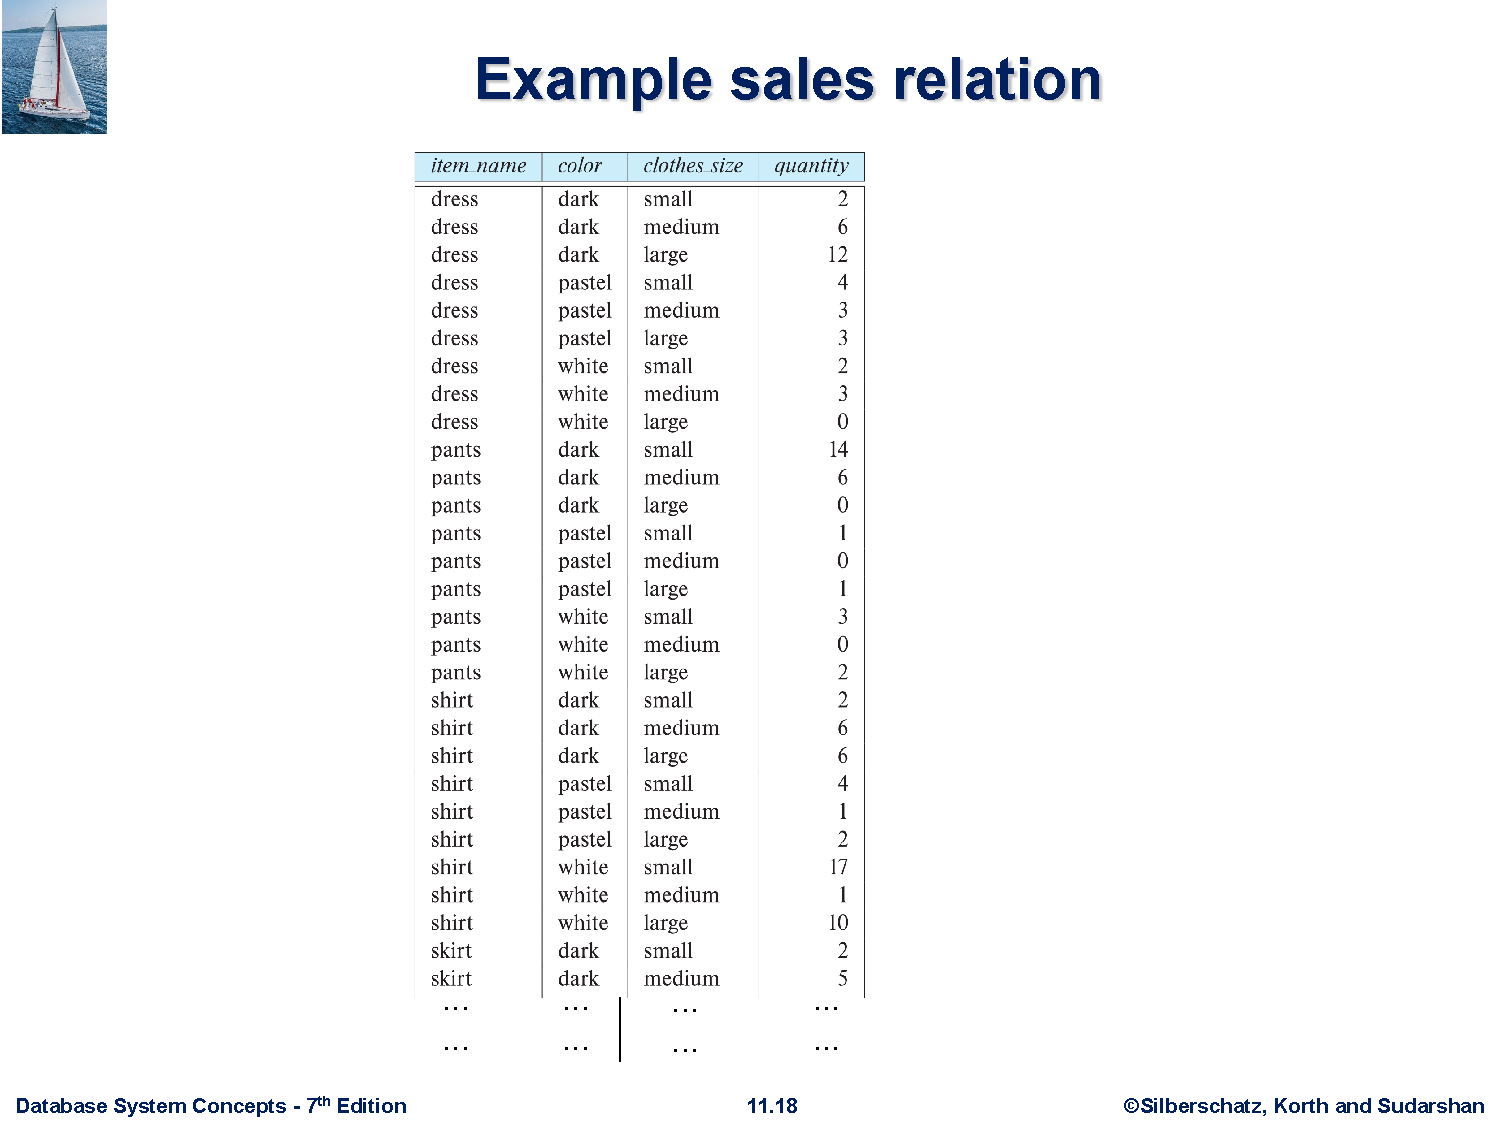
\includegraphics[width=\textwidth, trim={0cm 1cm 0cm 0cm}, clip]{slides/s18} }
\end{frame}
\begin{frame}{}
    \Wider{ 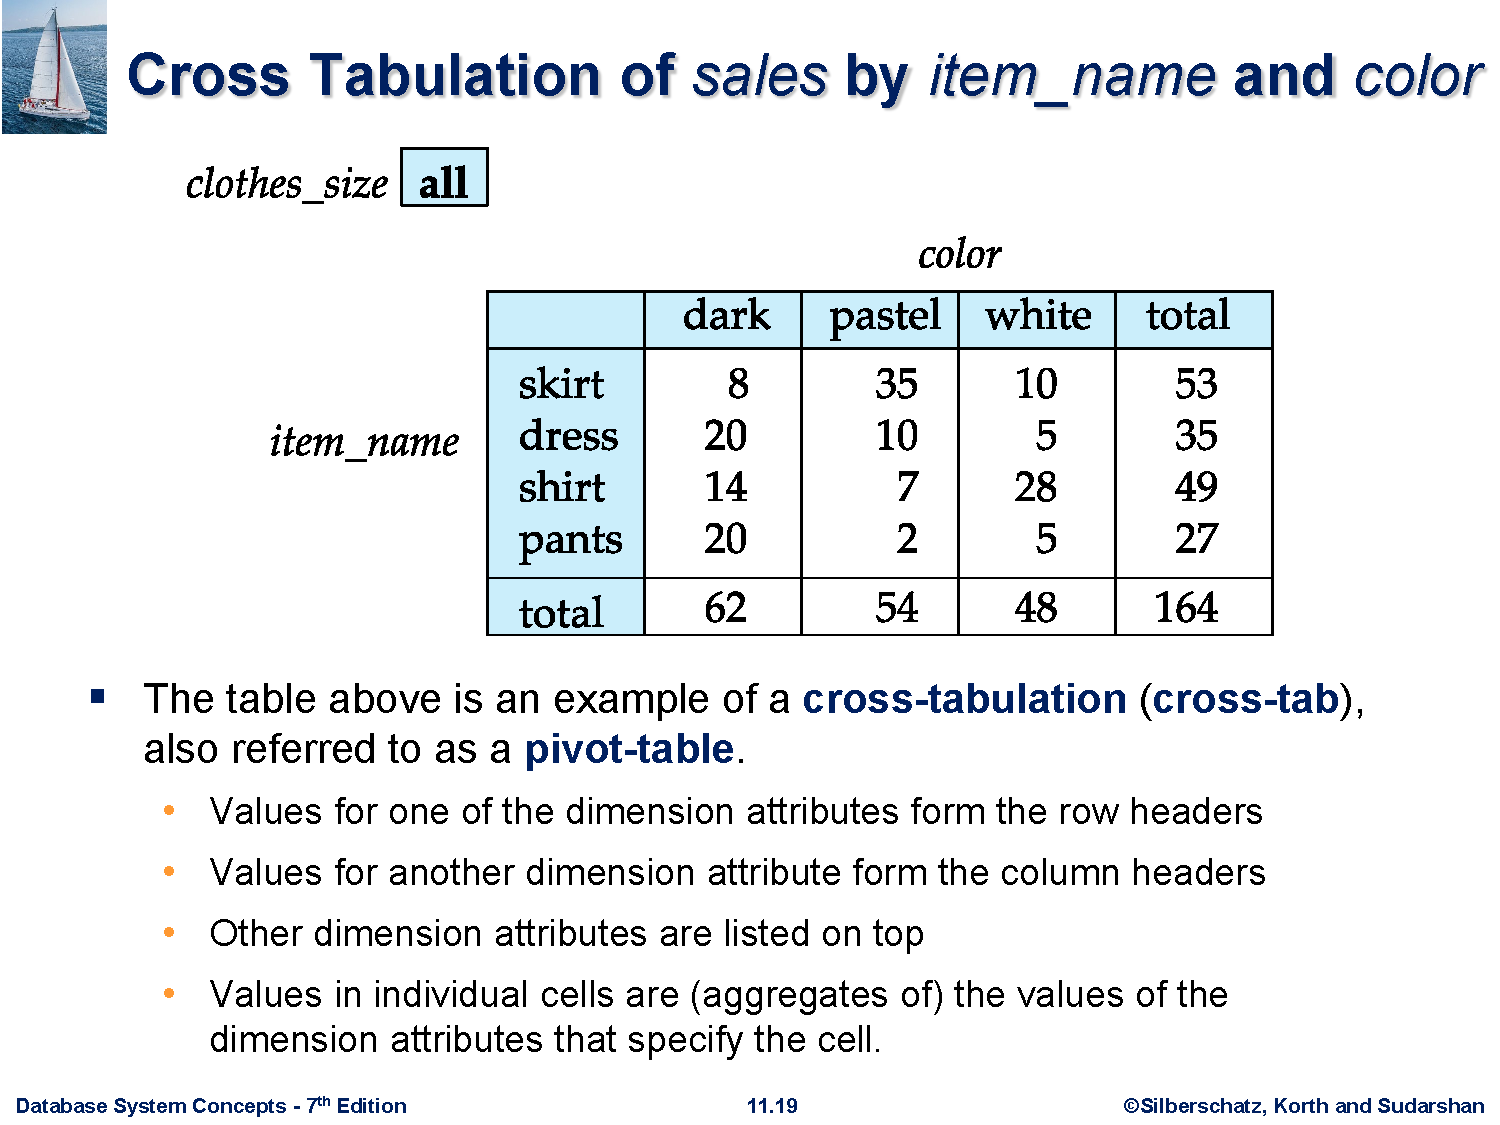
\includegraphics[width=\textwidth, trim={0cm 1cm 0cm 0cm}, clip]{slides/s19} }
\end{frame}
\begin{frame}{}
    \Wider{ 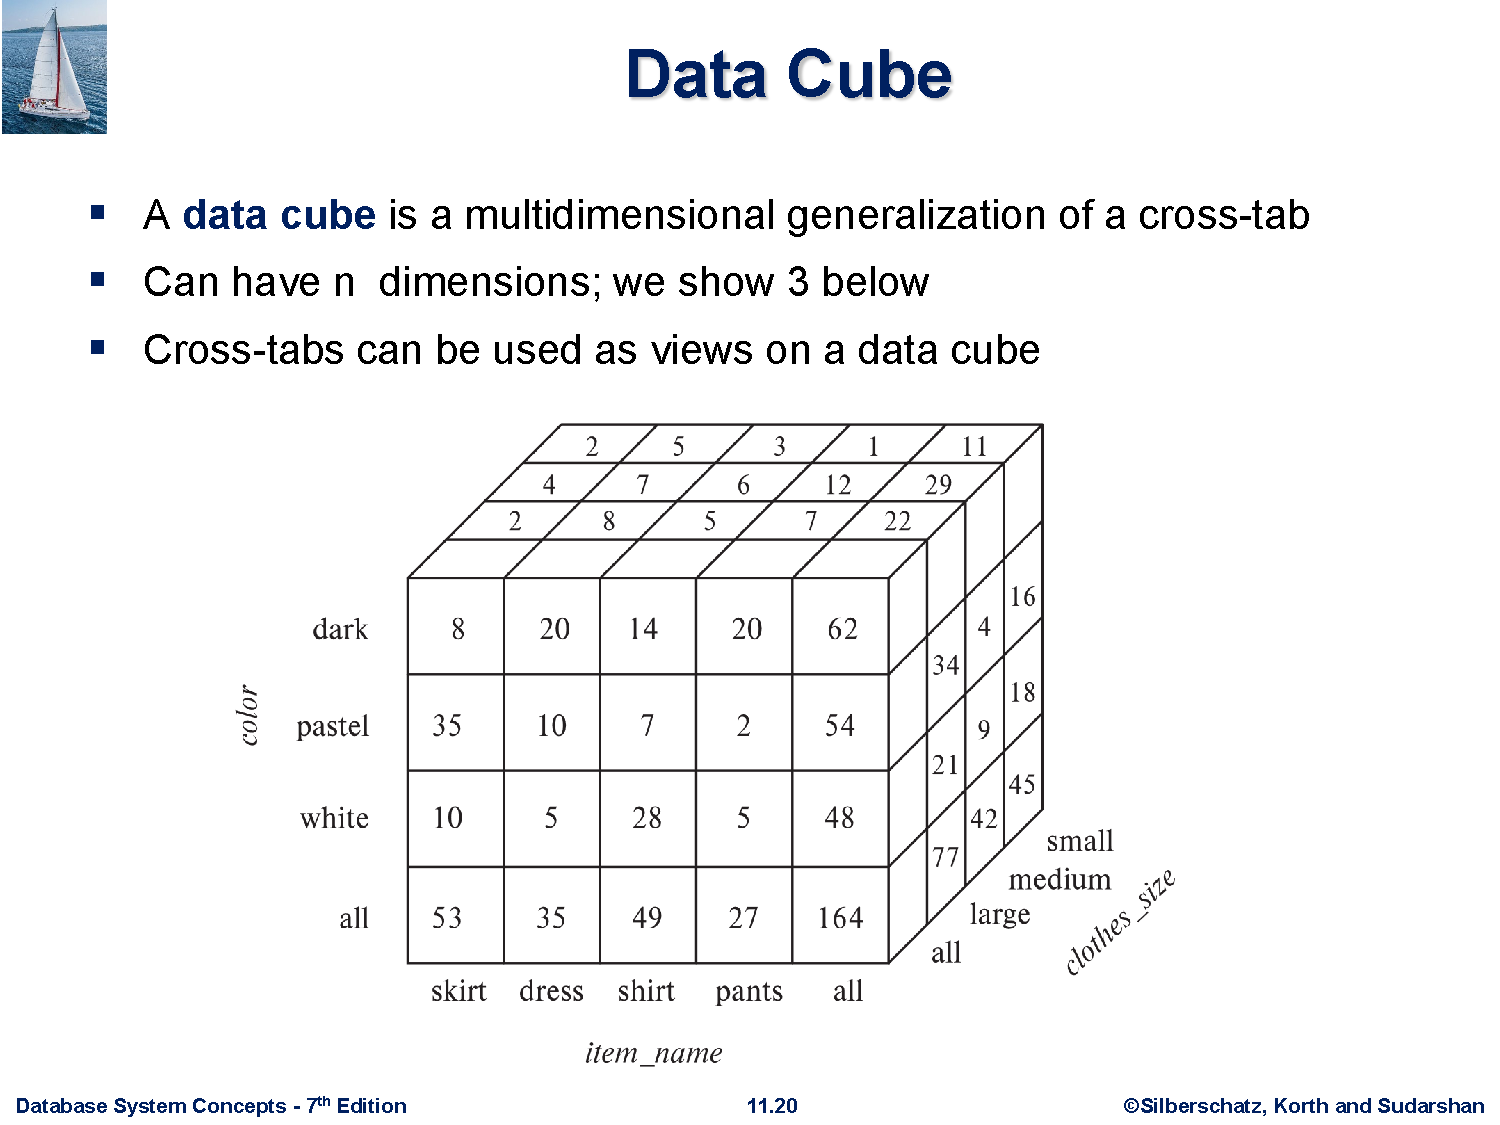
\includegraphics[width=\textwidth, trim={0cm 1cm 0cm 0cm}, clip]{slides/s20} }
\end{frame}
\begin{frame}{}
    \Wider{ 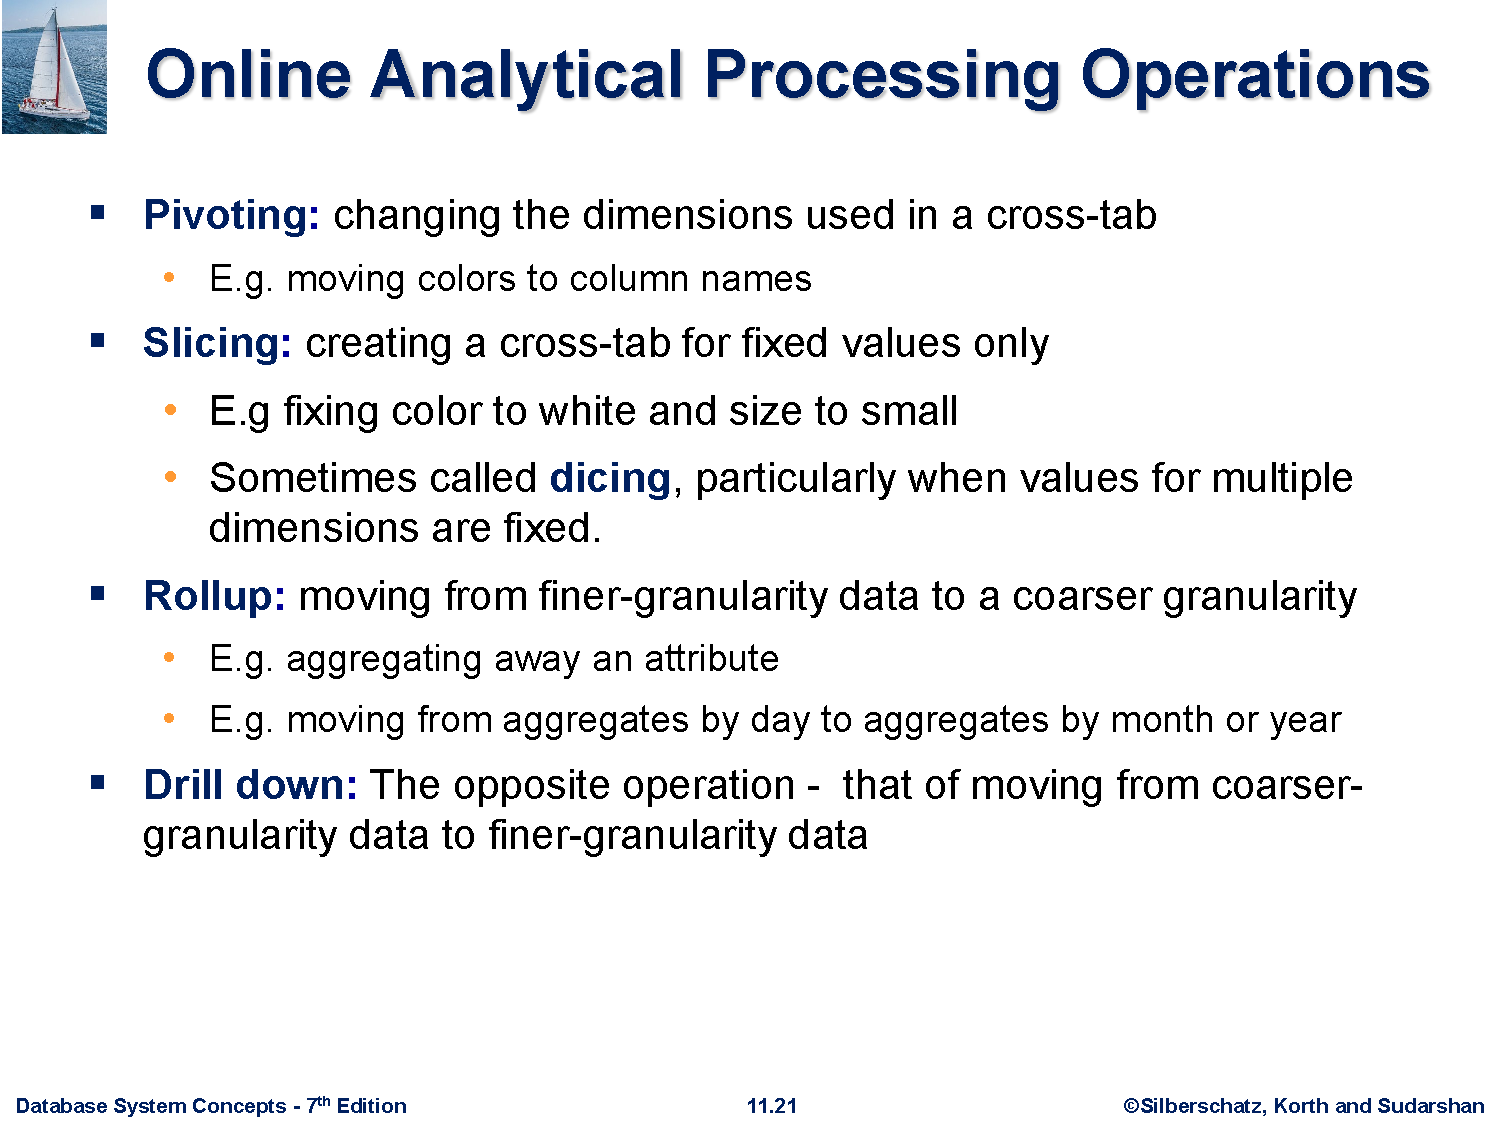
\includegraphics[width=\textwidth, trim={0cm 1cm 0cm 0cm}, clip]{slides/s21} }
\end{frame}
\begin{frame}{}
    \Wider{ 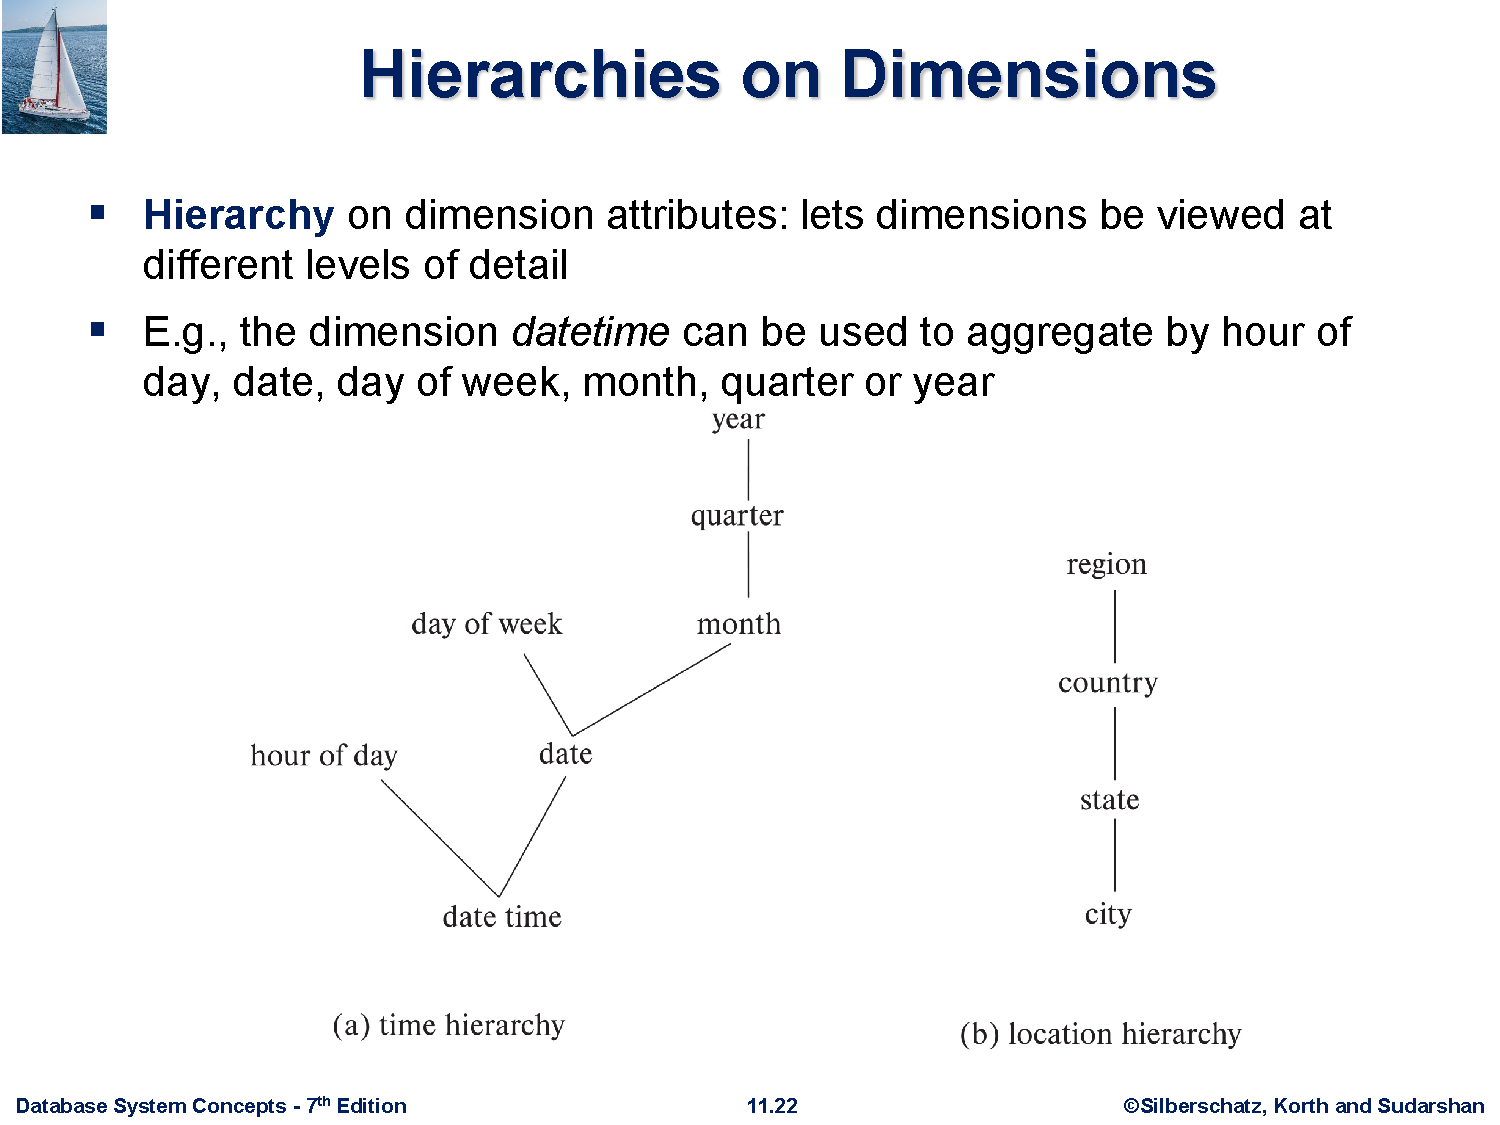
\includegraphics[width=\textwidth, trim={0cm 1cm 0cm 0cm}, clip]{slides/s22} }
\end{frame}
\begin{frame}{}
    \Wider{ 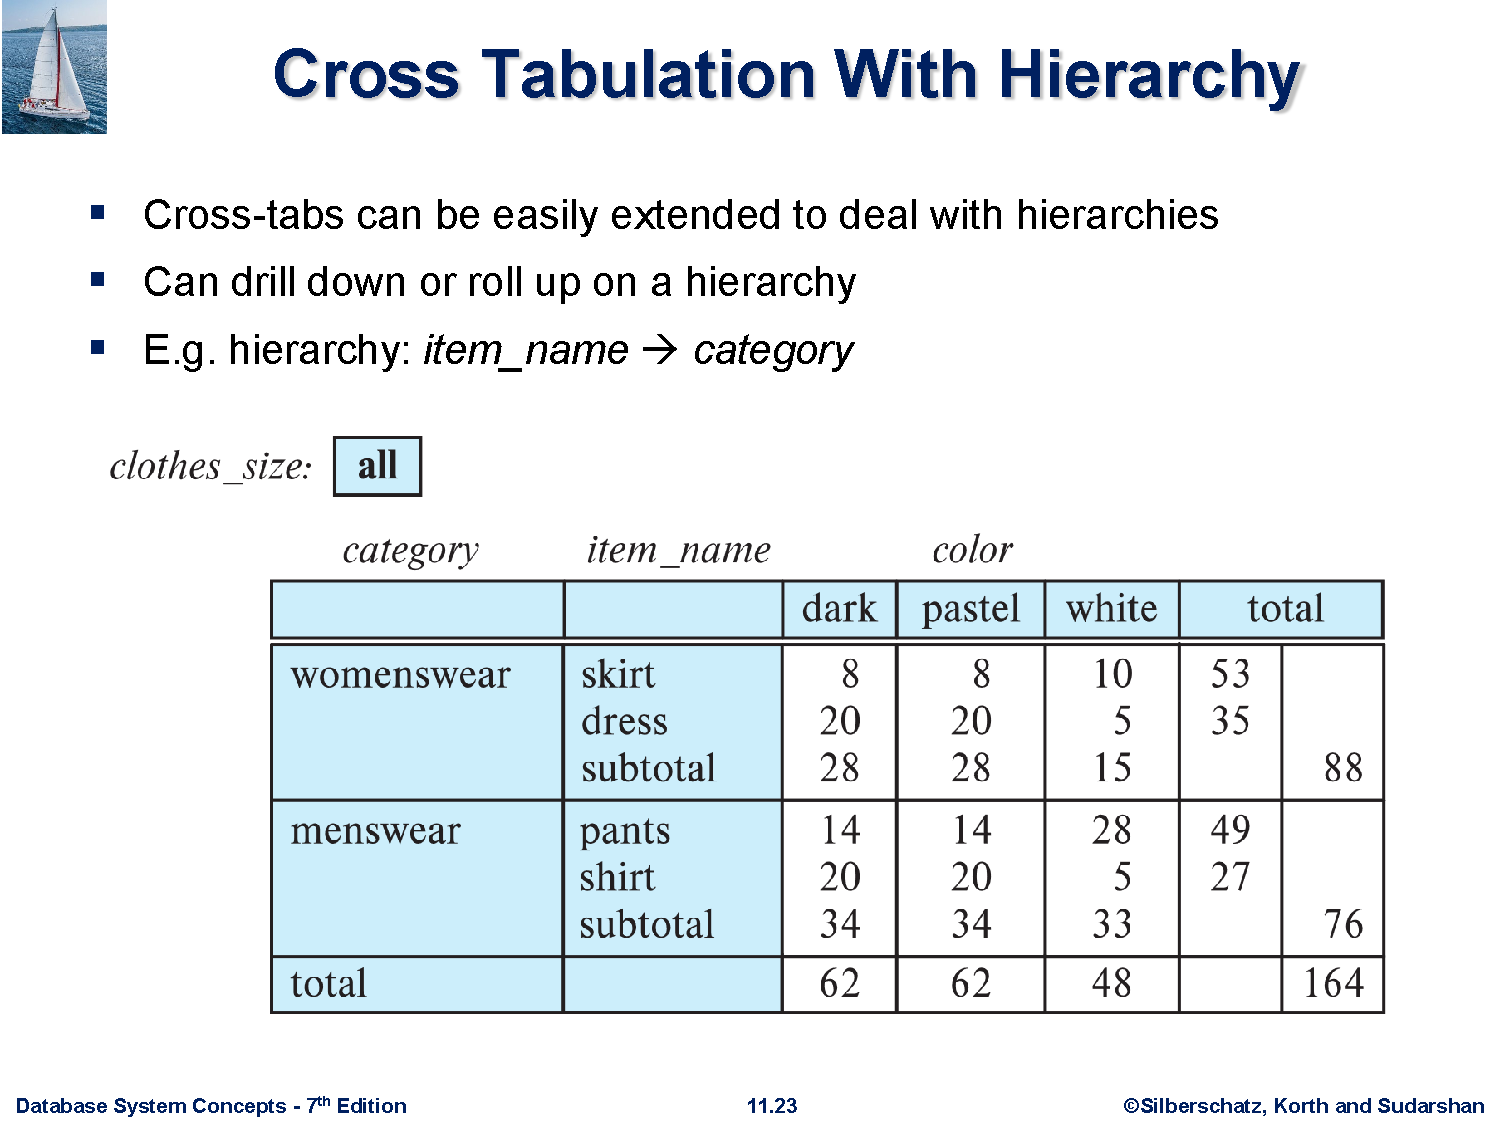
\includegraphics[width=\textwidth, trim={0cm 1cm 0cm 0cm}, clip]{slides/s23} }
\end{frame}
\begin{frame}{}
    \Wider{ 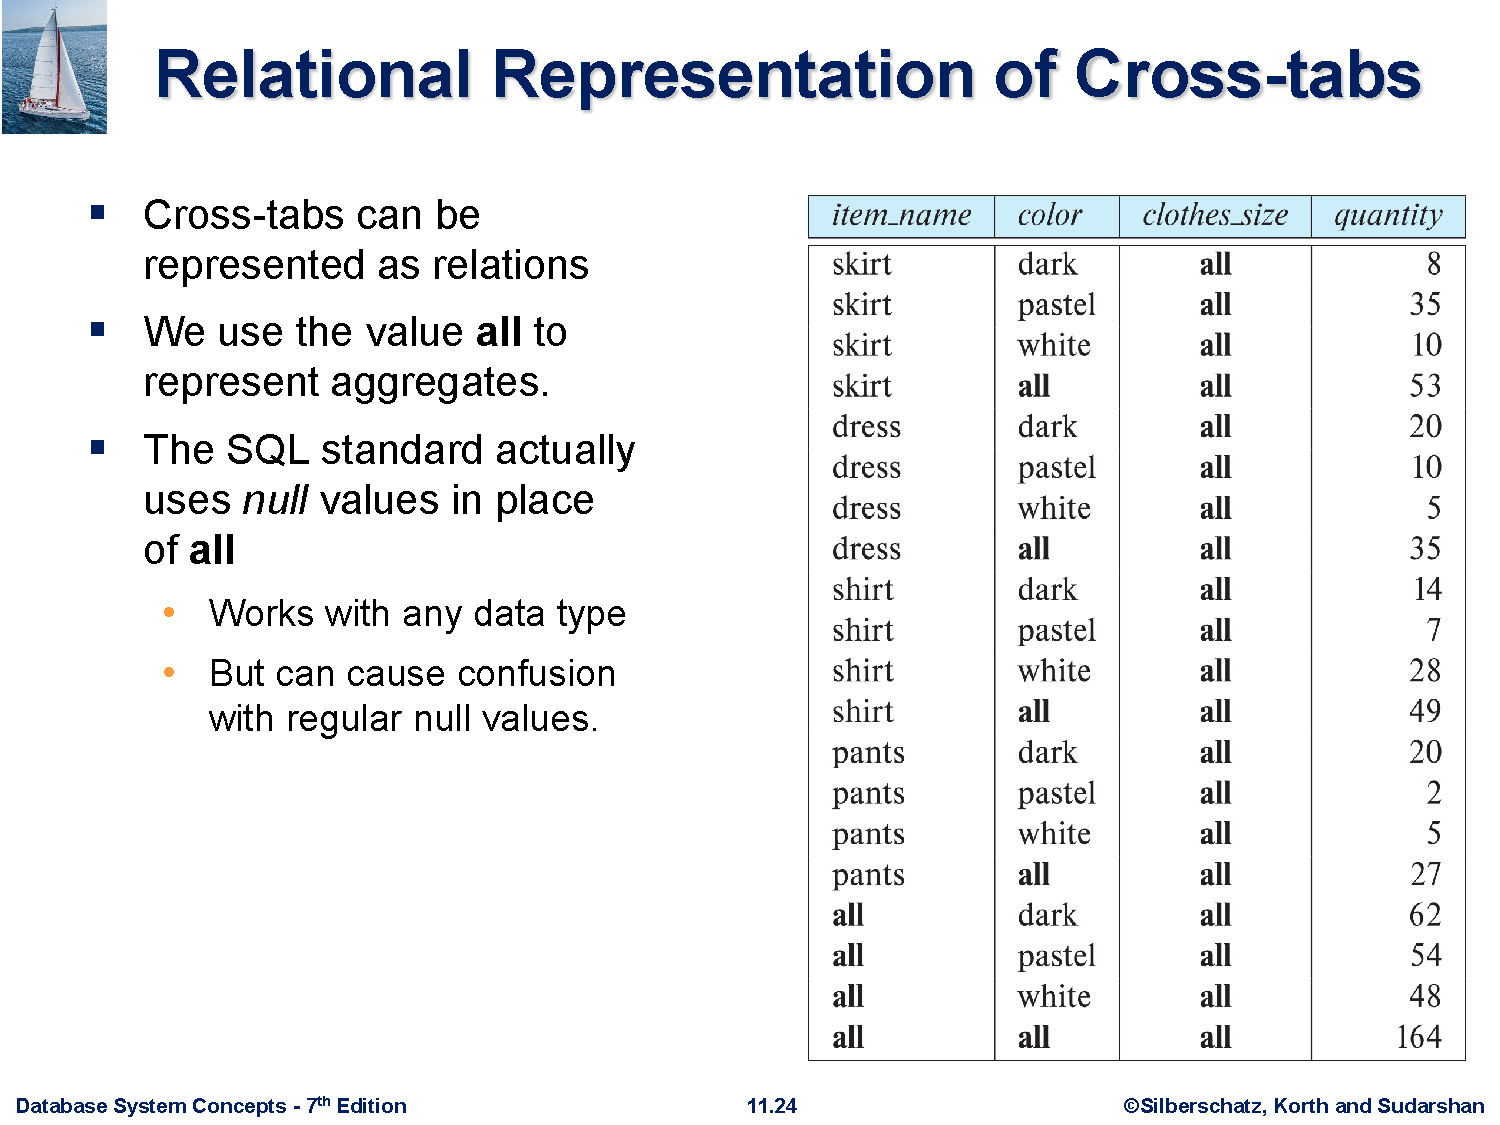
\includegraphics[width=\textwidth, trim={0cm 1cm 0cm 0cm}, clip]{slides/s24} }
\end{frame}

% \section{OLAP in SQL}
%
% \begin{frame}{}
%     \Wider{ 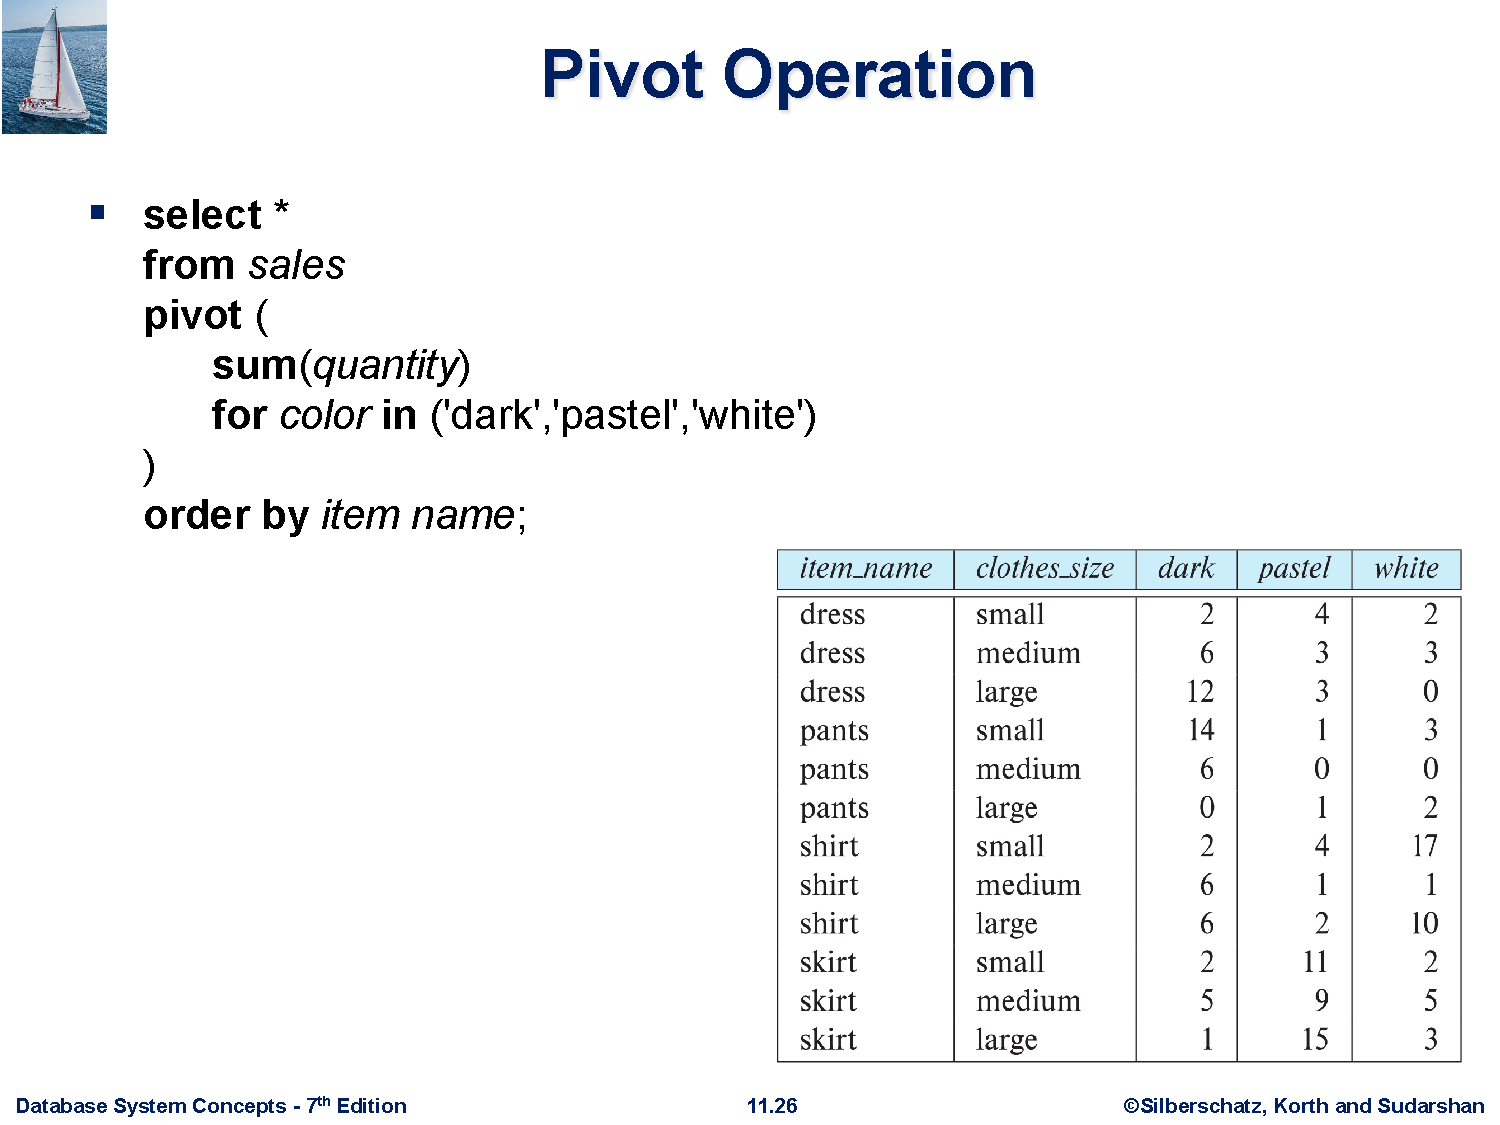
\includegraphics[width=\textwidth, trim={0cm 1cm 0cm 0cm}, clip]{slides/s26} }
% \end{frame}
% \begin{frame}{}
%     \Wider{ 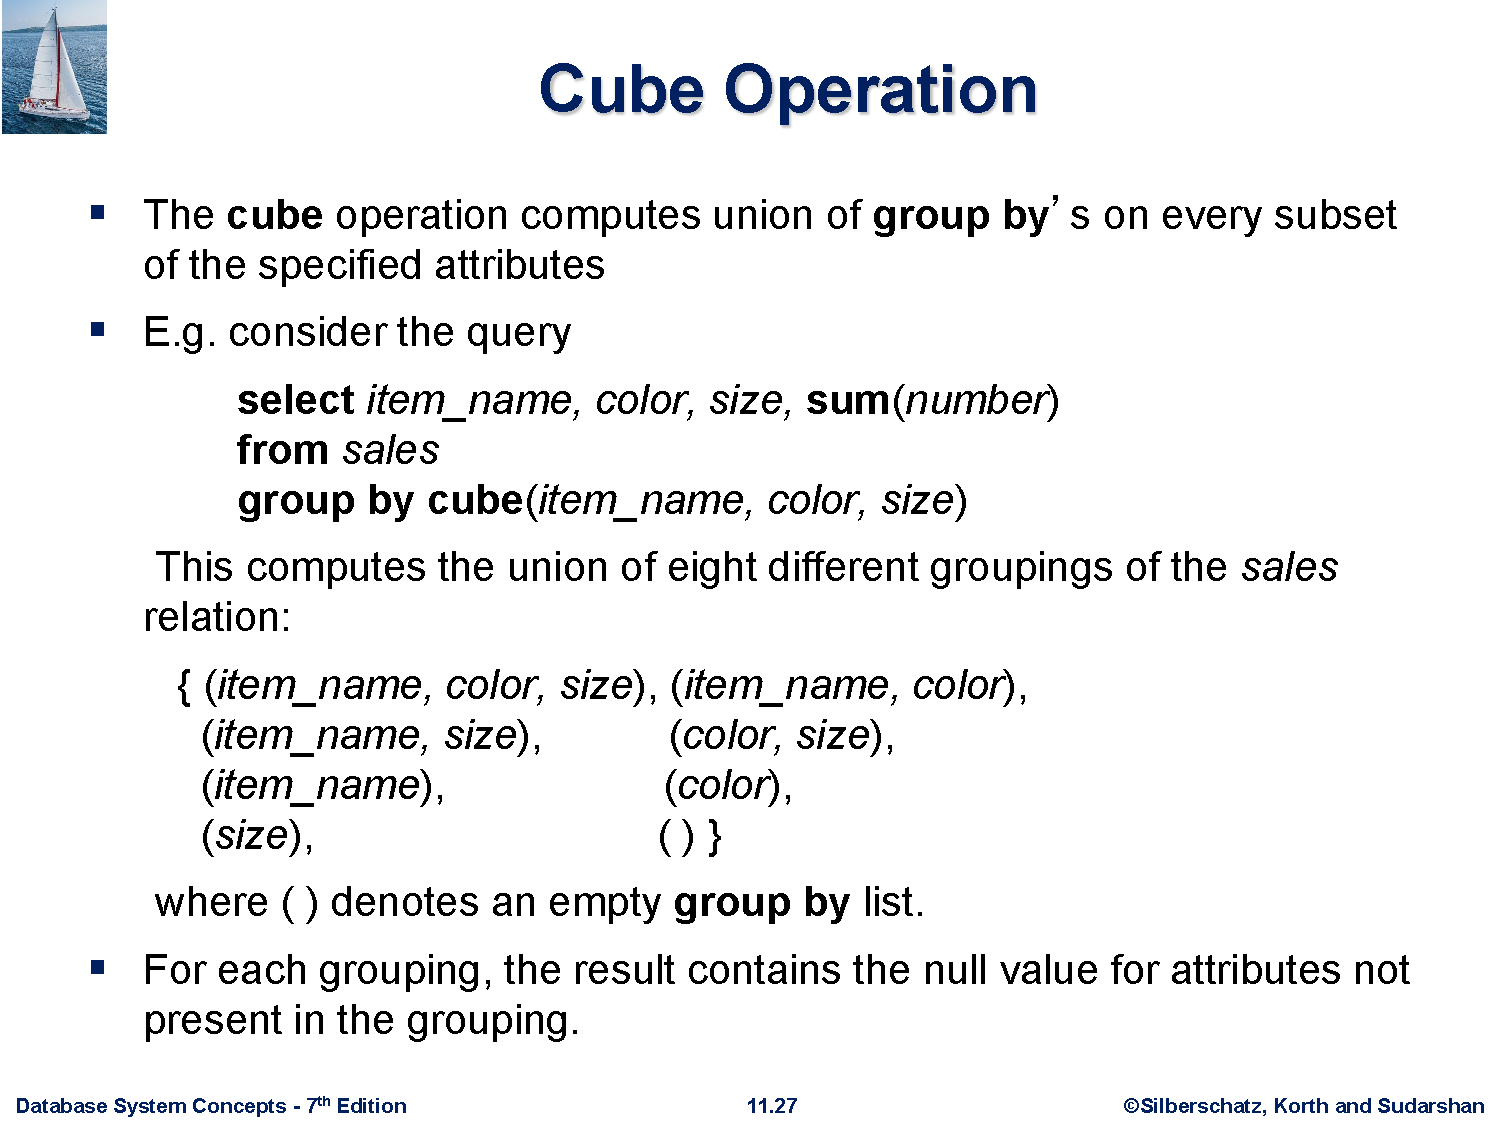
\includegraphics[width=\textwidth, trim={0cm 1cm 0cm 0cm}, clip]{slides/s27} }
% \end{frame}
% \begin{frame}{}
%     \Wider{ 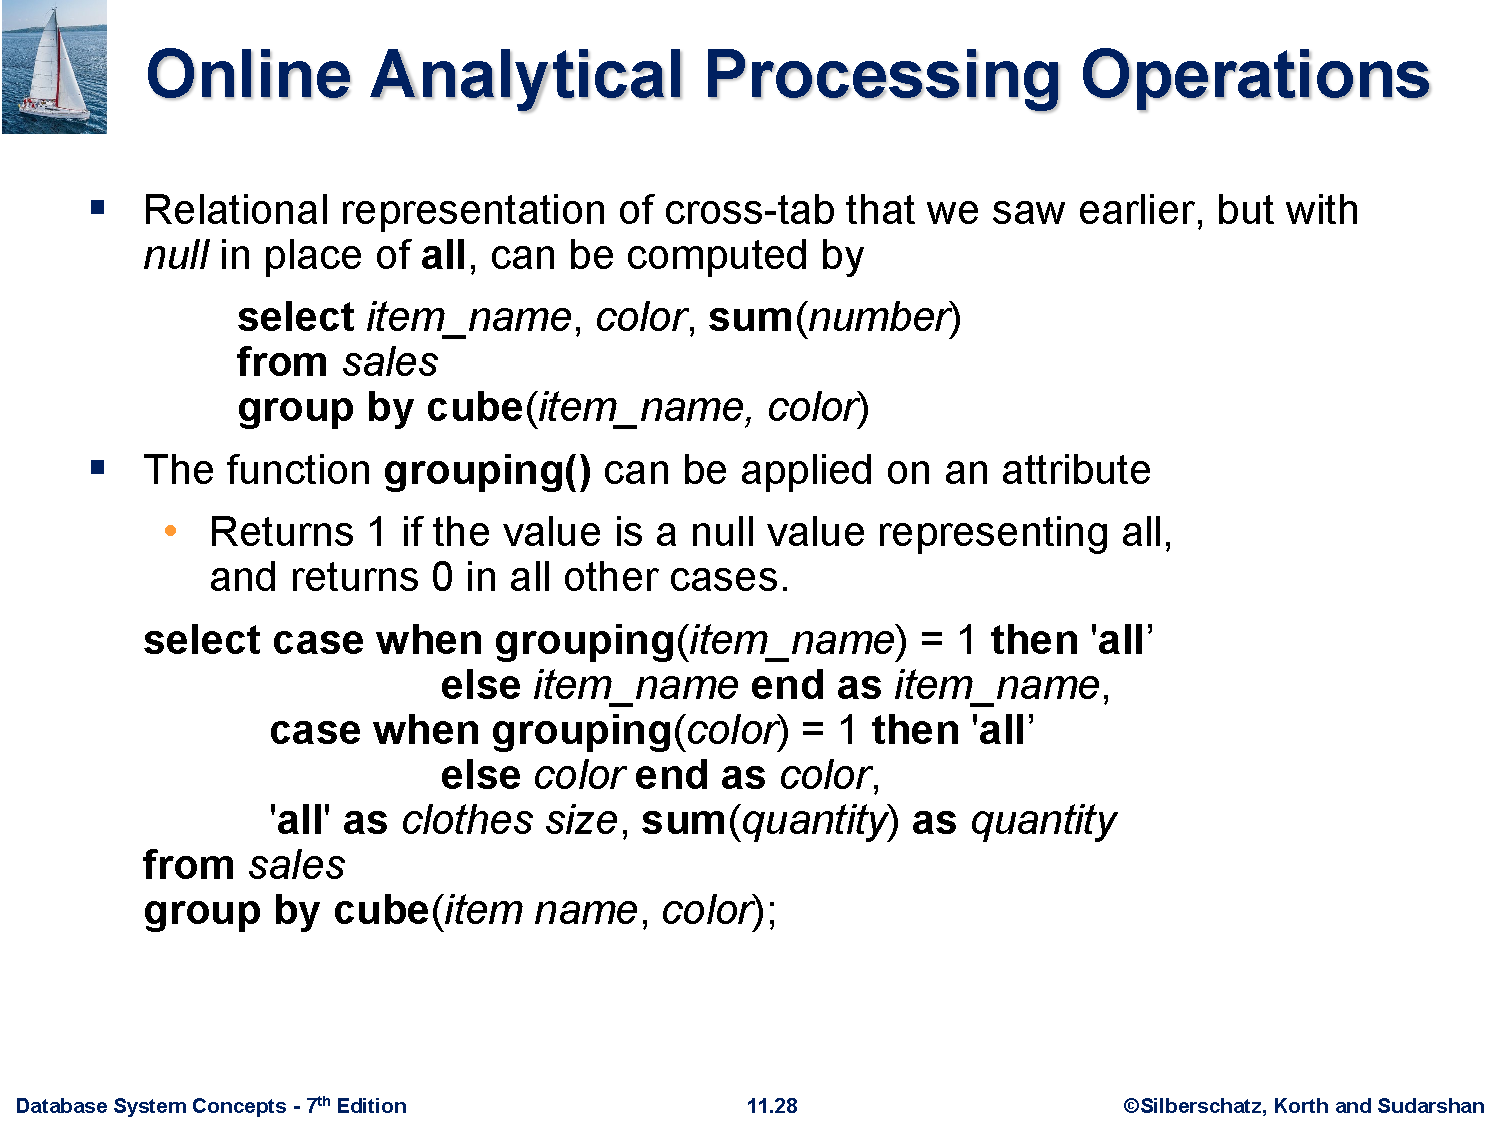
\includegraphics[width=\textwidth, trim={0cm 1cm 0cm 0cm}, clip]{slides/s28} }
% \end{frame}
% \begin{frame}{}
%     \Wider{ 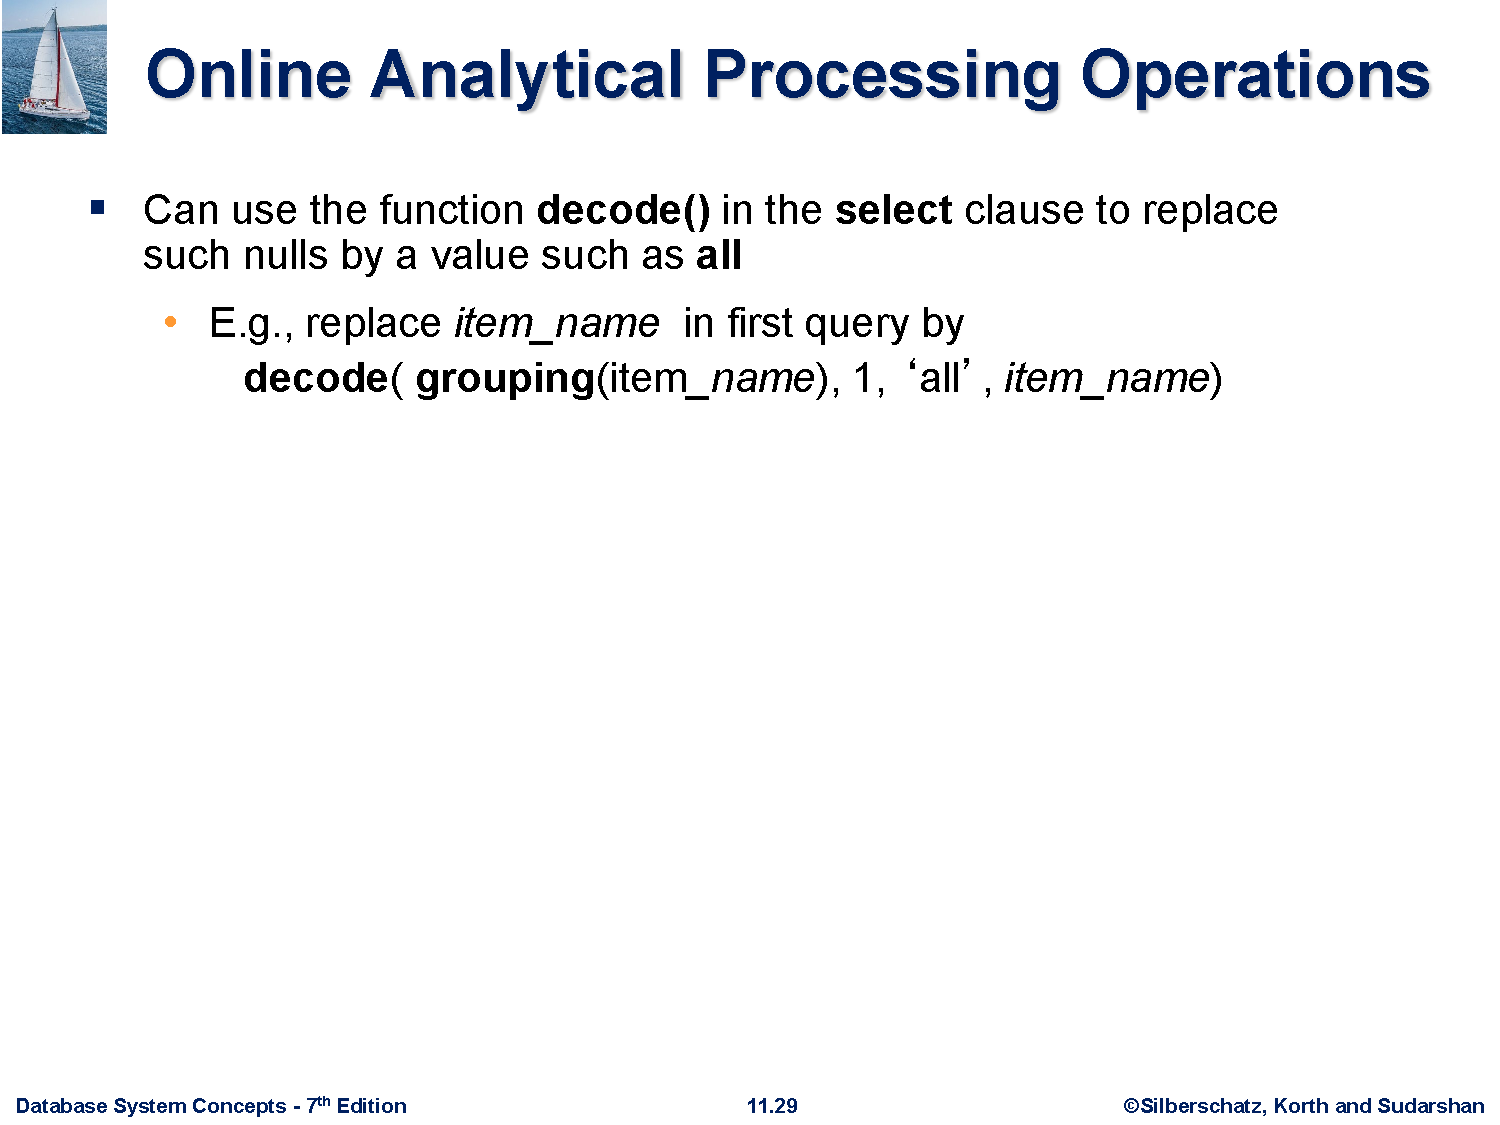
\includegraphics[width=\textwidth, trim={0cm 1cm 0cm 0cm}, clip]{slides/s29} }
% \end{frame}
% \begin{frame}{}
%     \Wider{ 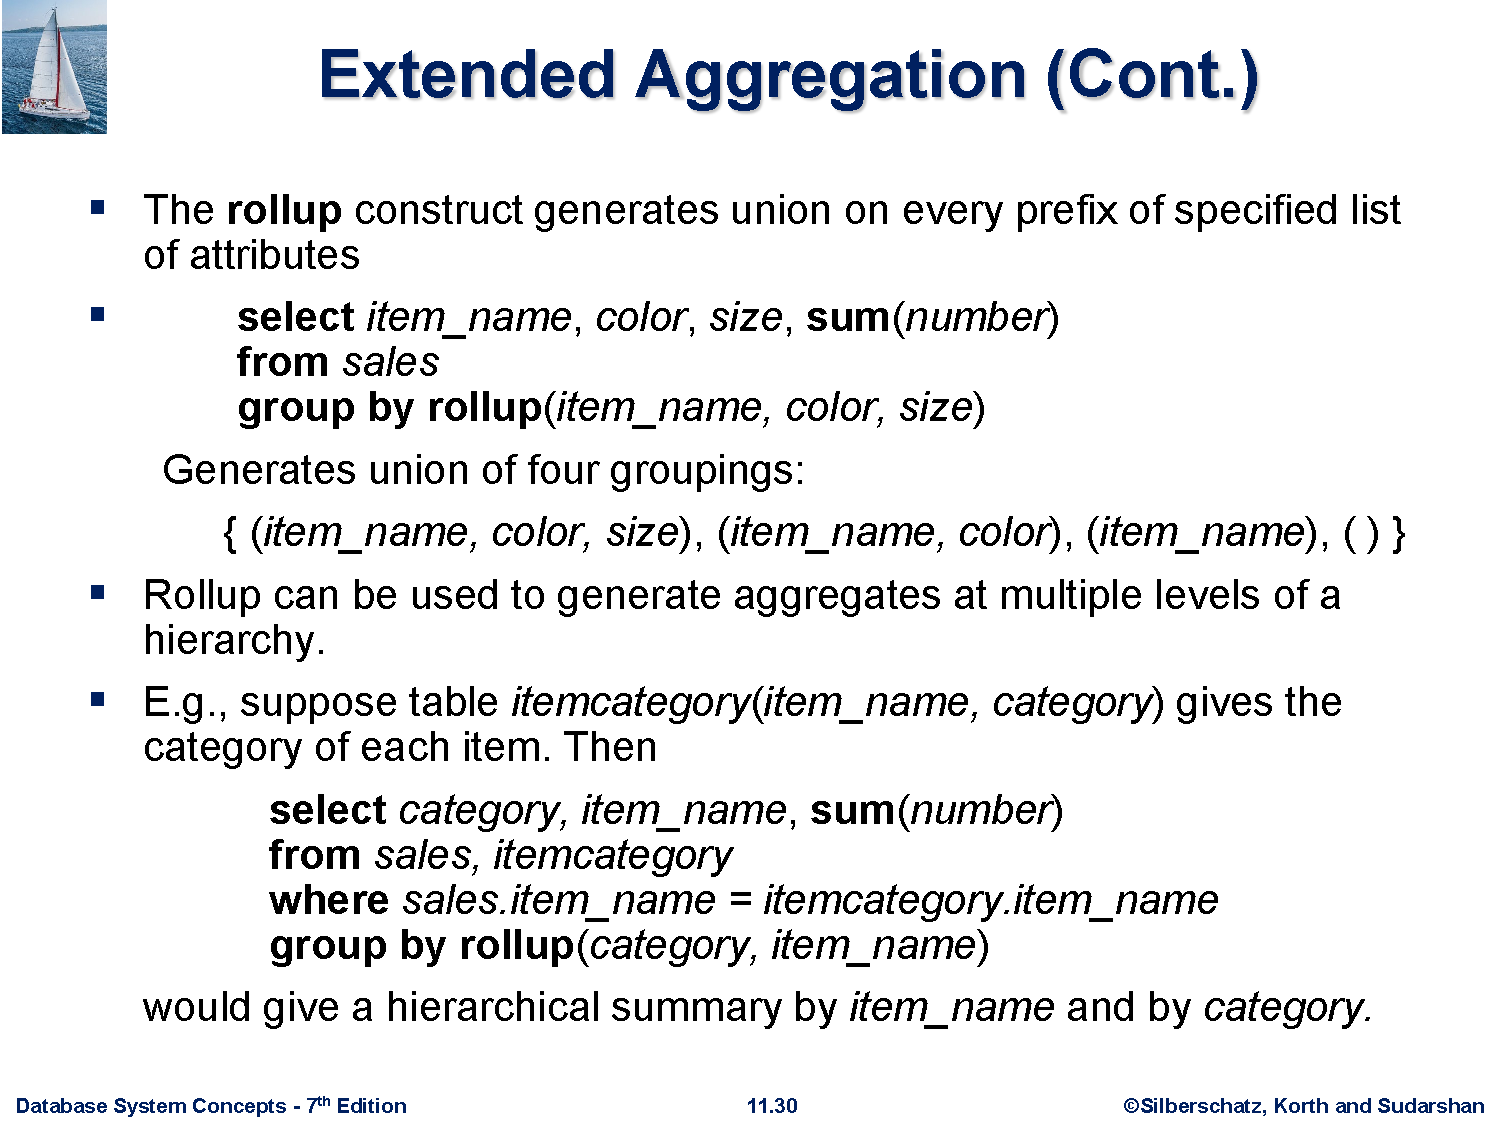
\includegraphics[width=\textwidth, trim={0cm 1cm 0cm 0cm}, clip]{slides/s30} }
% \end{frame}
% \begin{frame}{}
%     \Wider{ 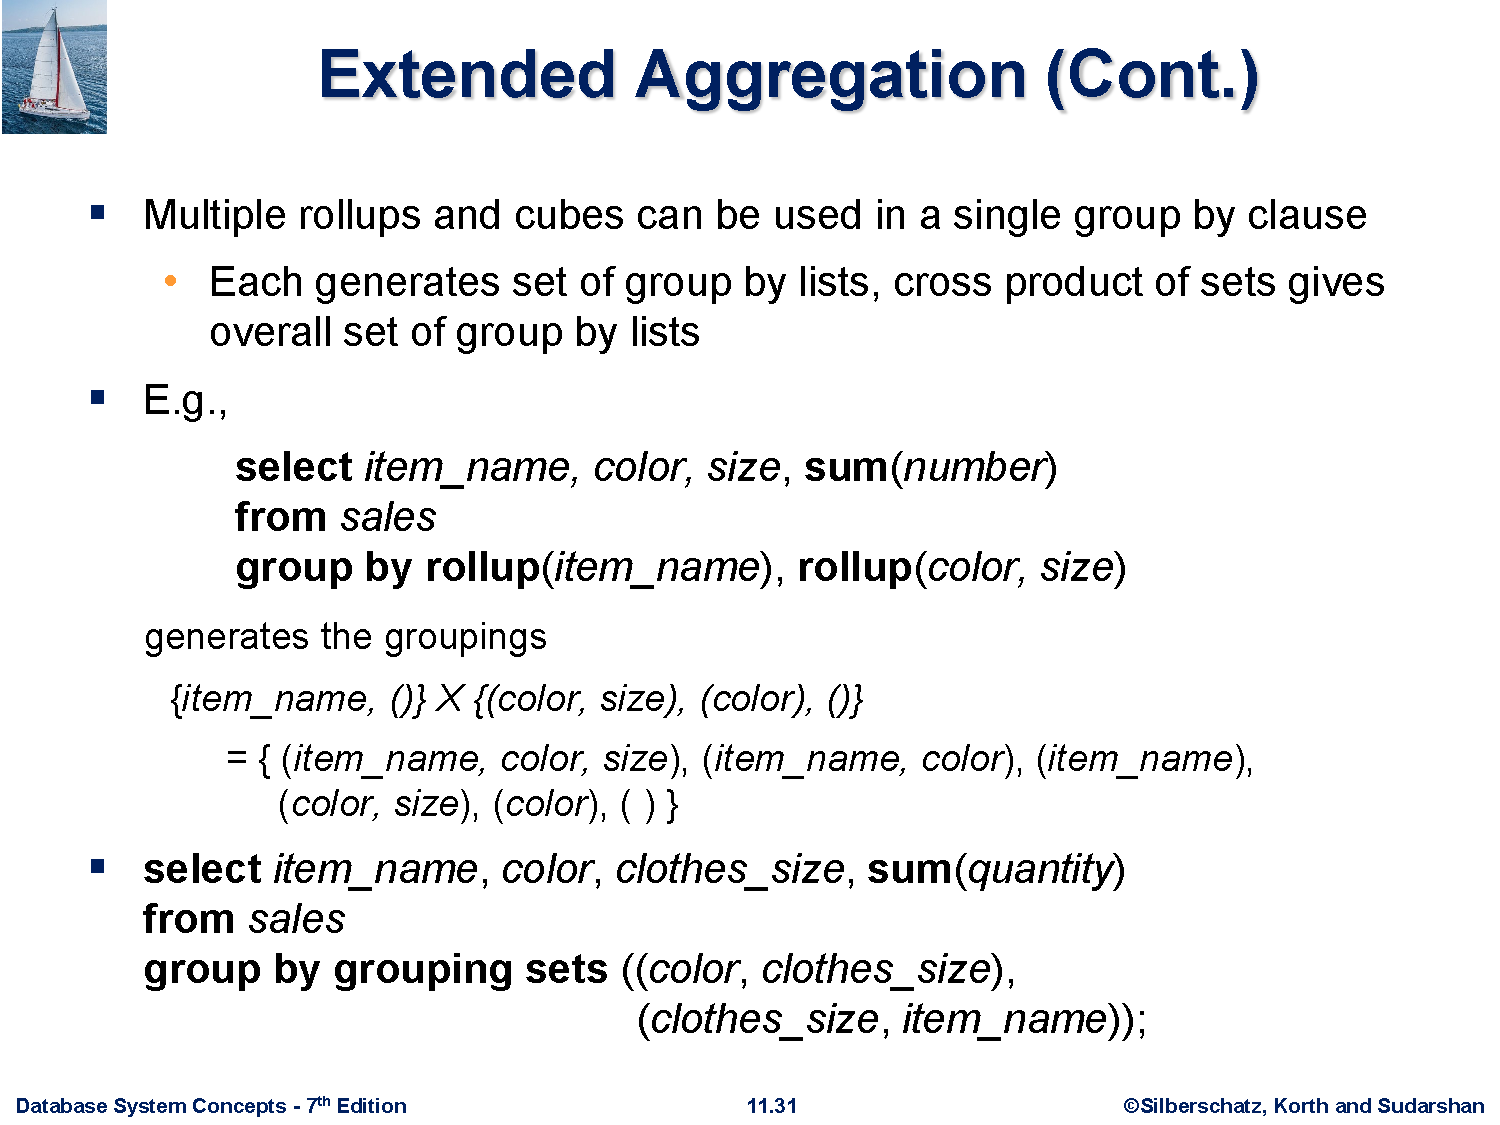
\includegraphics[width=\textwidth, trim={0cm 1cm 0cm 0cm}, clip]{slides/s31} }
% \end{frame}
% \begin{frame}{}
%     \Wider{ 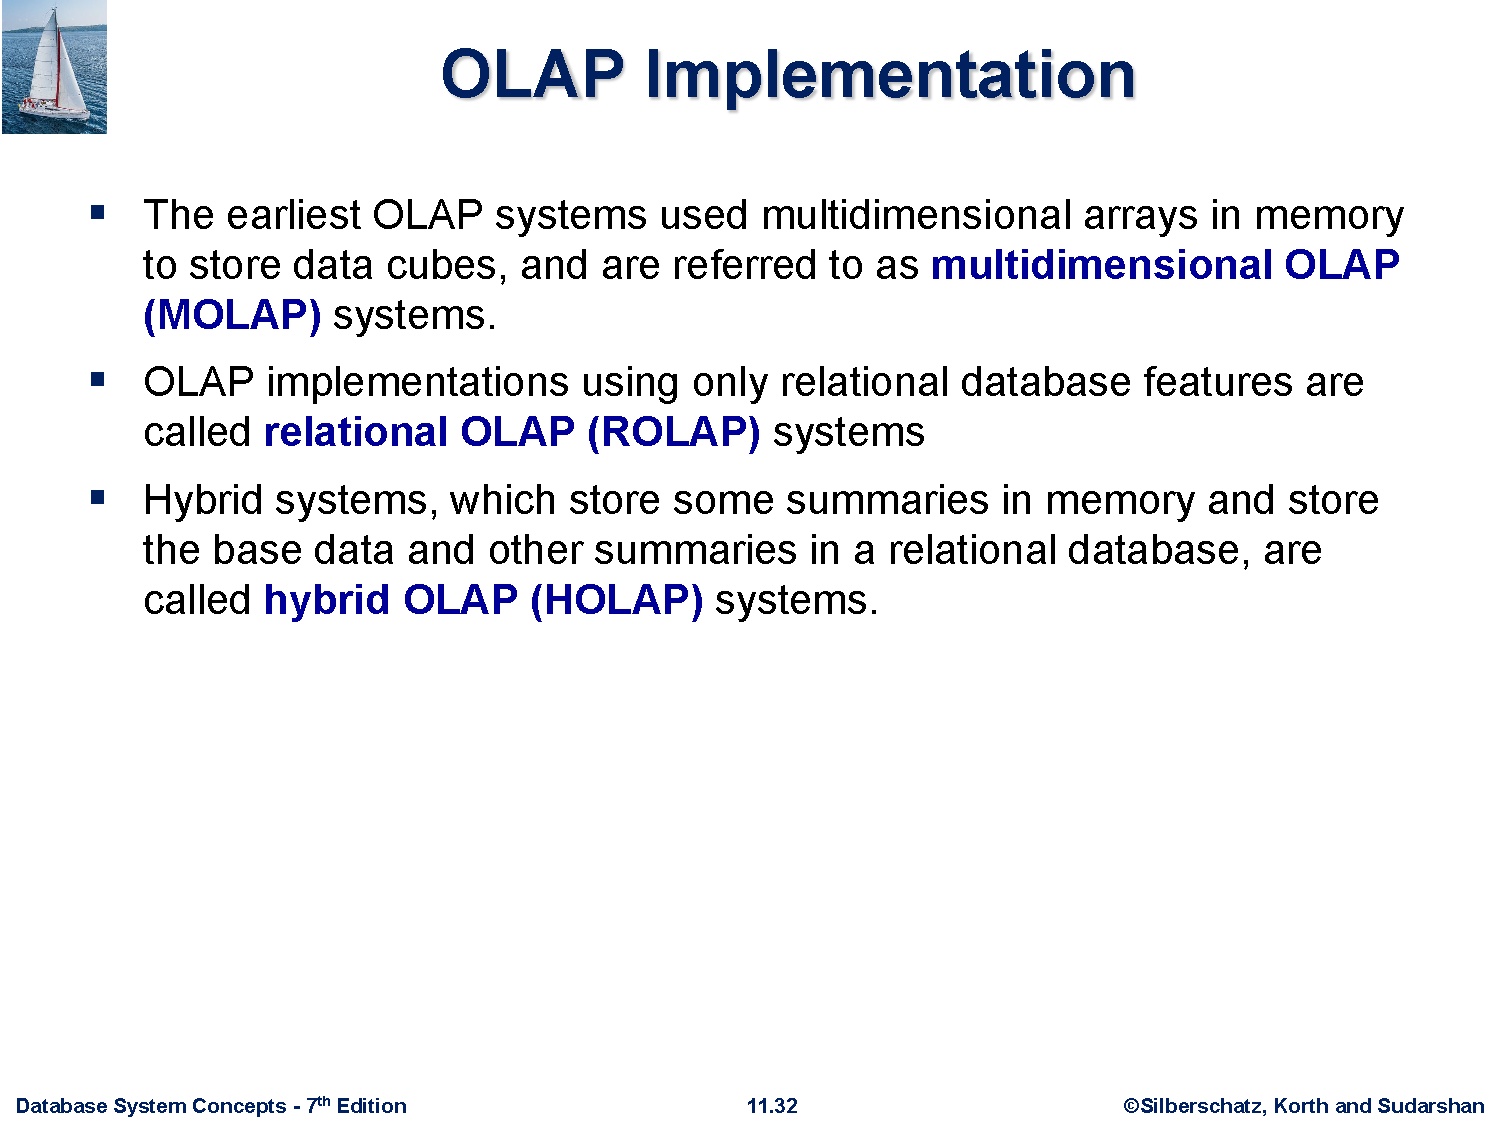
\includegraphics[width=\textwidth, trim={0cm 1cm 0cm 0cm}, clip]{slides/s32} }
% \end{frame}
% \begin{frame}{}
%     \Wider{ 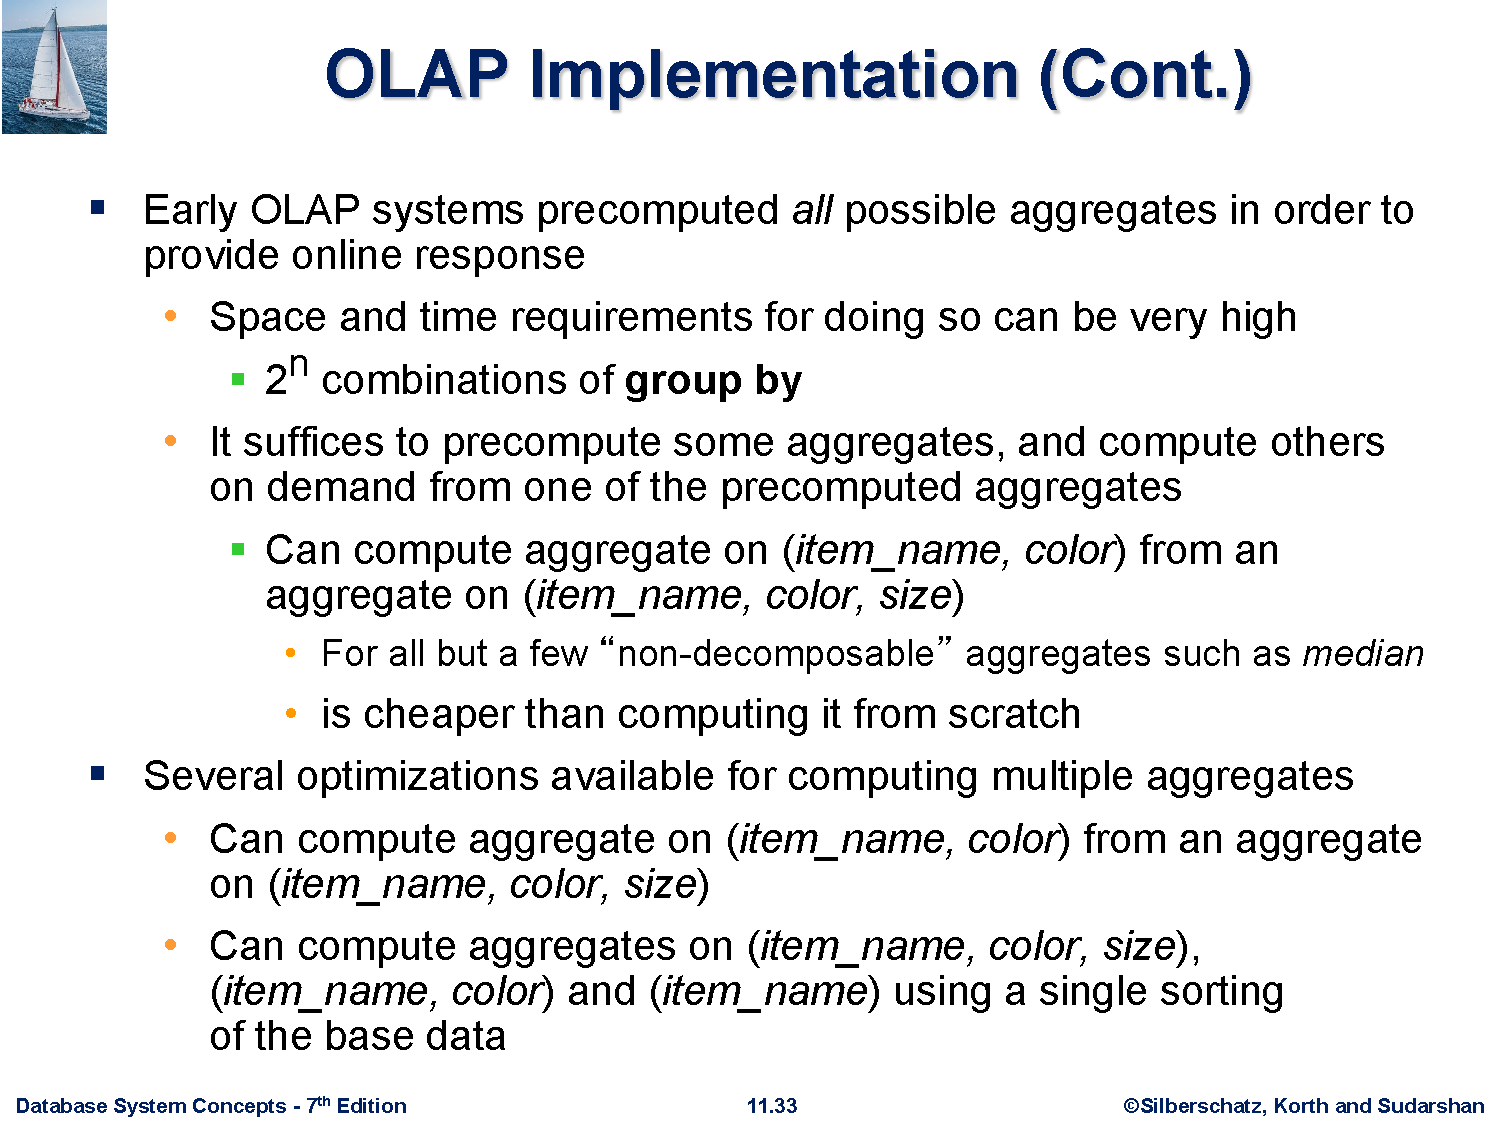
\includegraphics[width=\textwidth, trim={0cm 1cm 0cm 0cm}, clip]{slides/s33} }
% \end{frame}
% \begin{frame}{}
%     \Wider{ 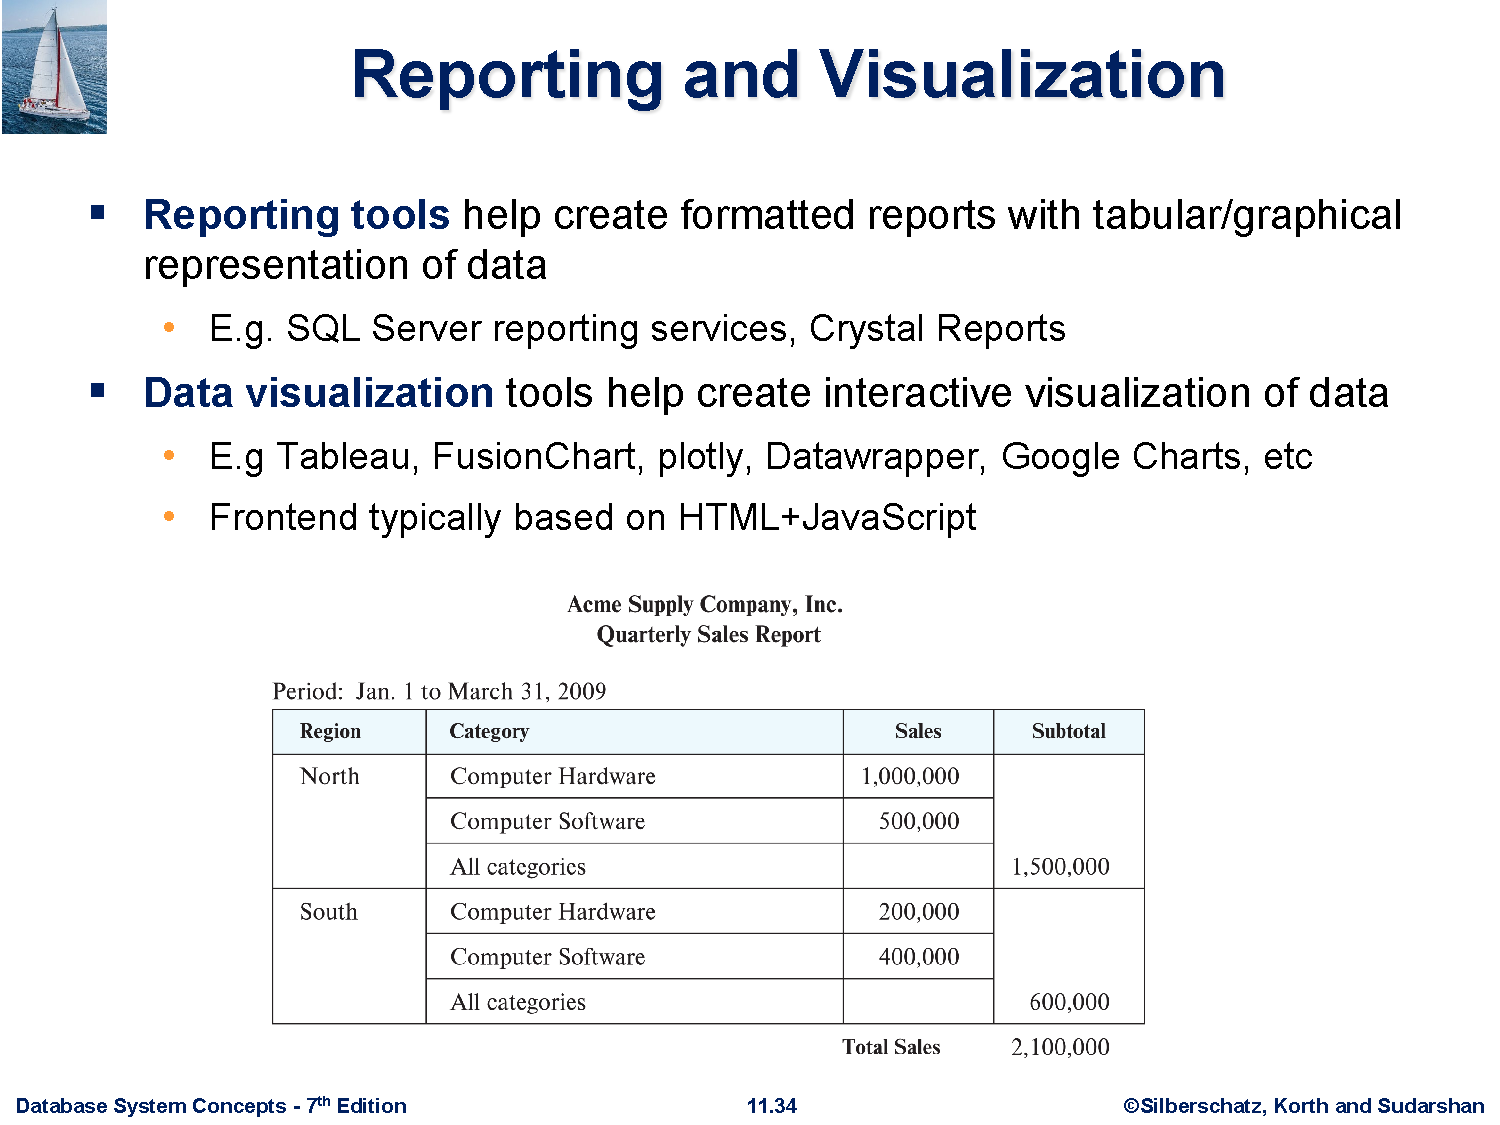
\includegraphics[width=\textwidth, trim={0cm 1cm 0cm 0cm}, clip]{slides/s34} }
% \end{frame}

\section{Data Mining}

\begin{frame}{}
    \Wider{ 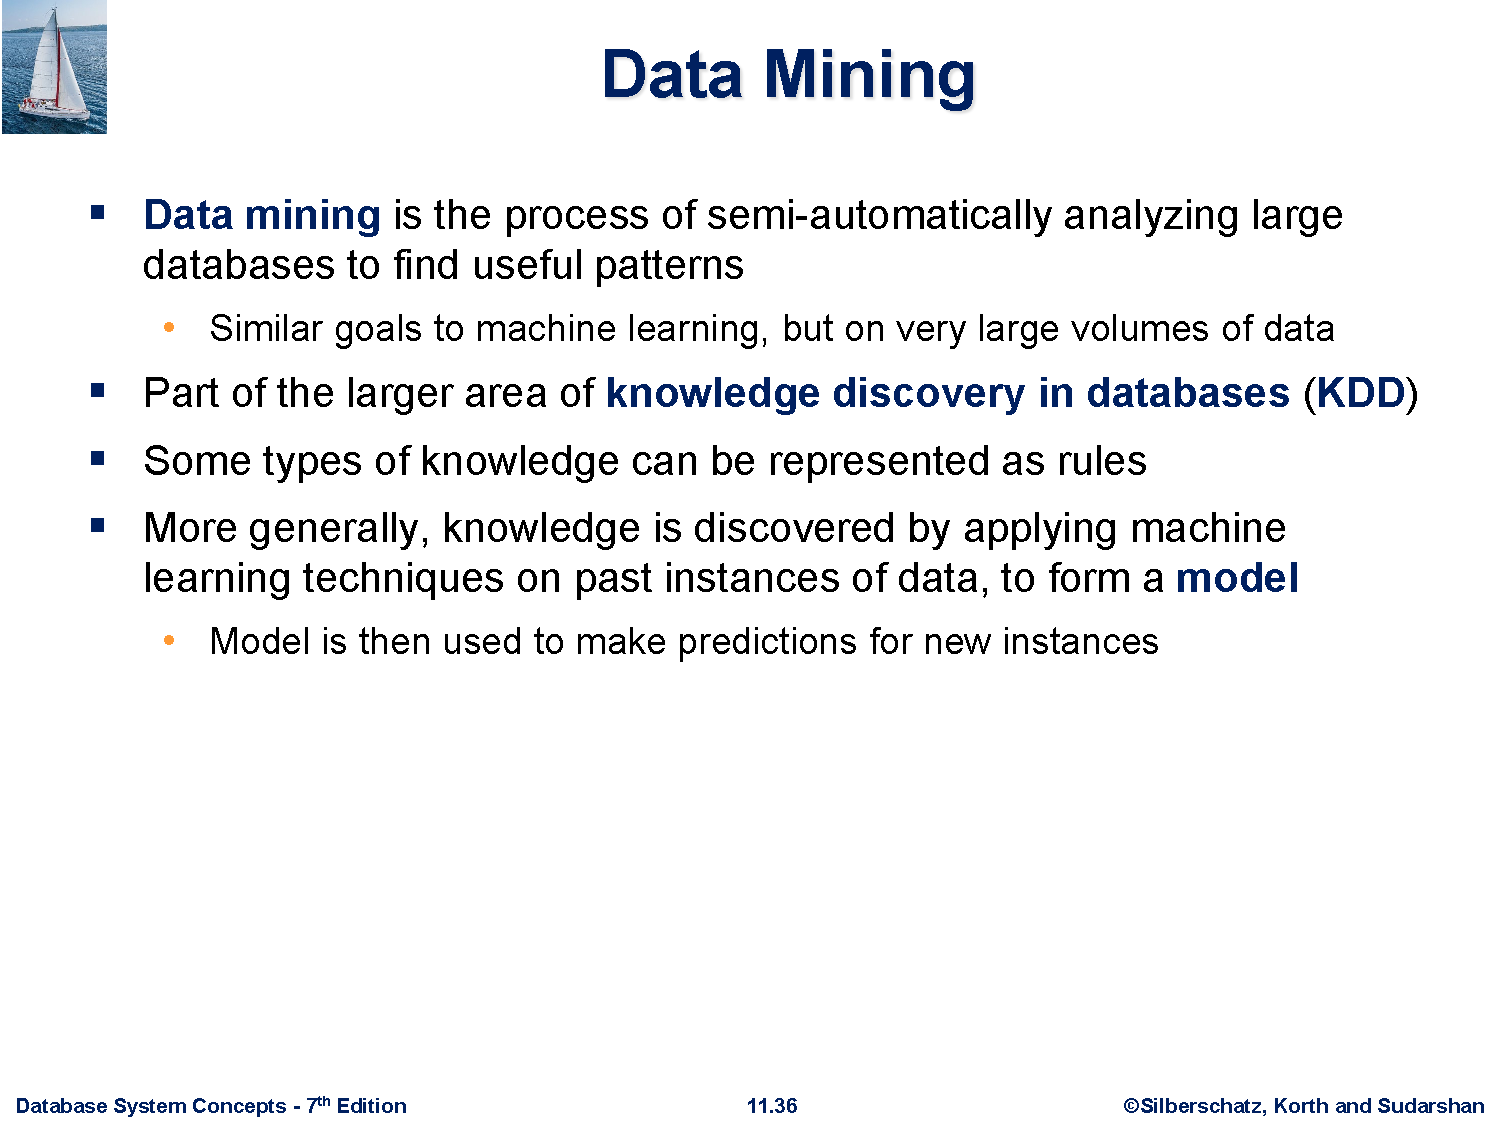
\includegraphics[width=\textwidth, trim={0cm 1cm 0cm 0cm}, clip]{slides/s36} }
\end{frame}
\begin{frame}{}
    \Wider{ 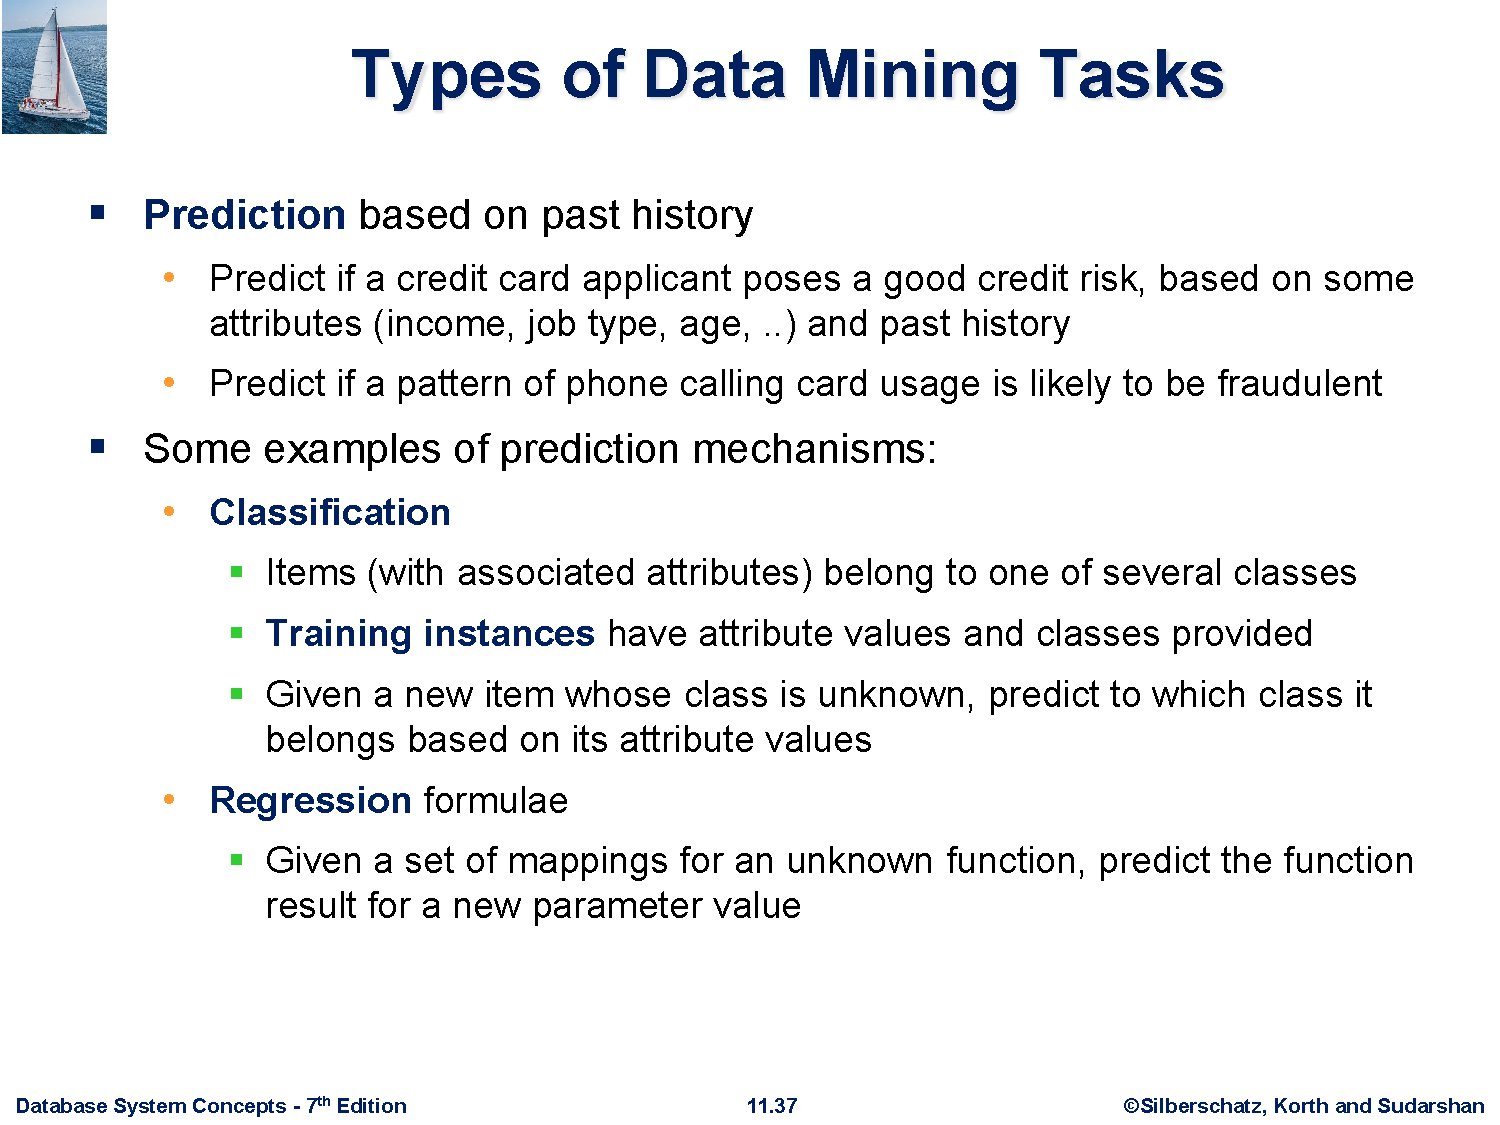
\includegraphics[width=\textwidth, trim={0cm 1cm 0cm 0cm}, clip]{slides/s37} }
\end{frame}
\begin{frame}{}
    \Wider{ 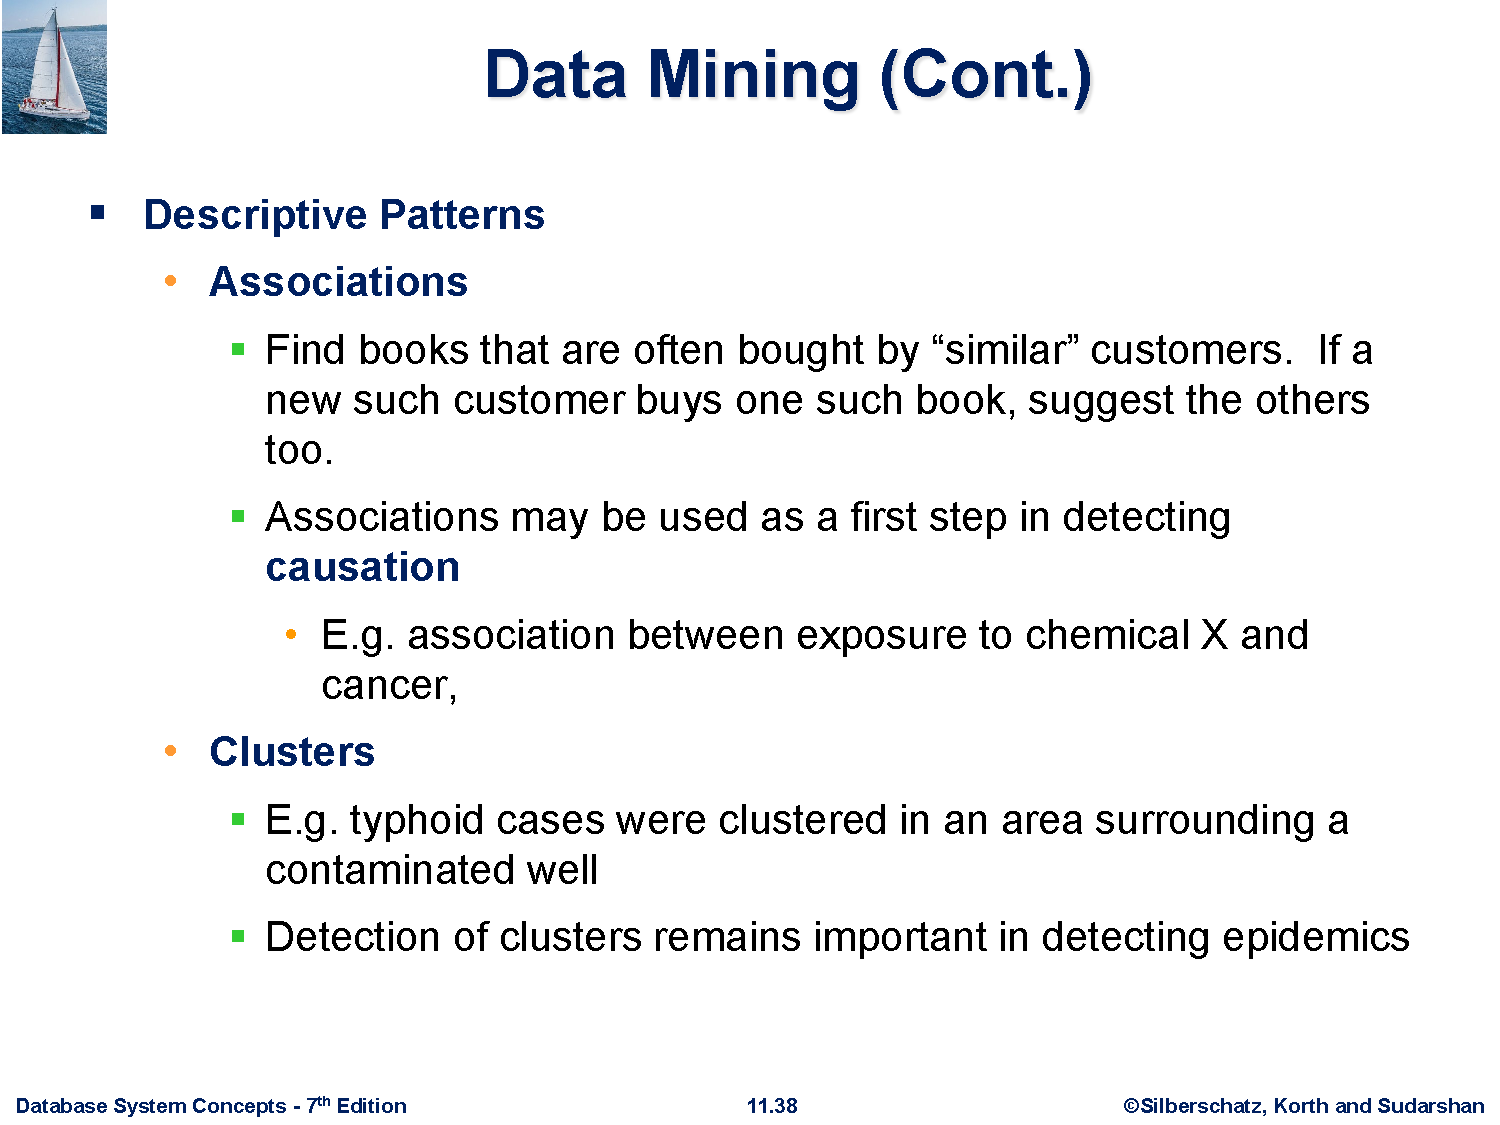
\includegraphics[width=\textwidth, trim={0cm 1cm 0cm 0cm}, clip]{slides/s38} }
\end{frame}
\begin{frame}{}
    \Wider{ 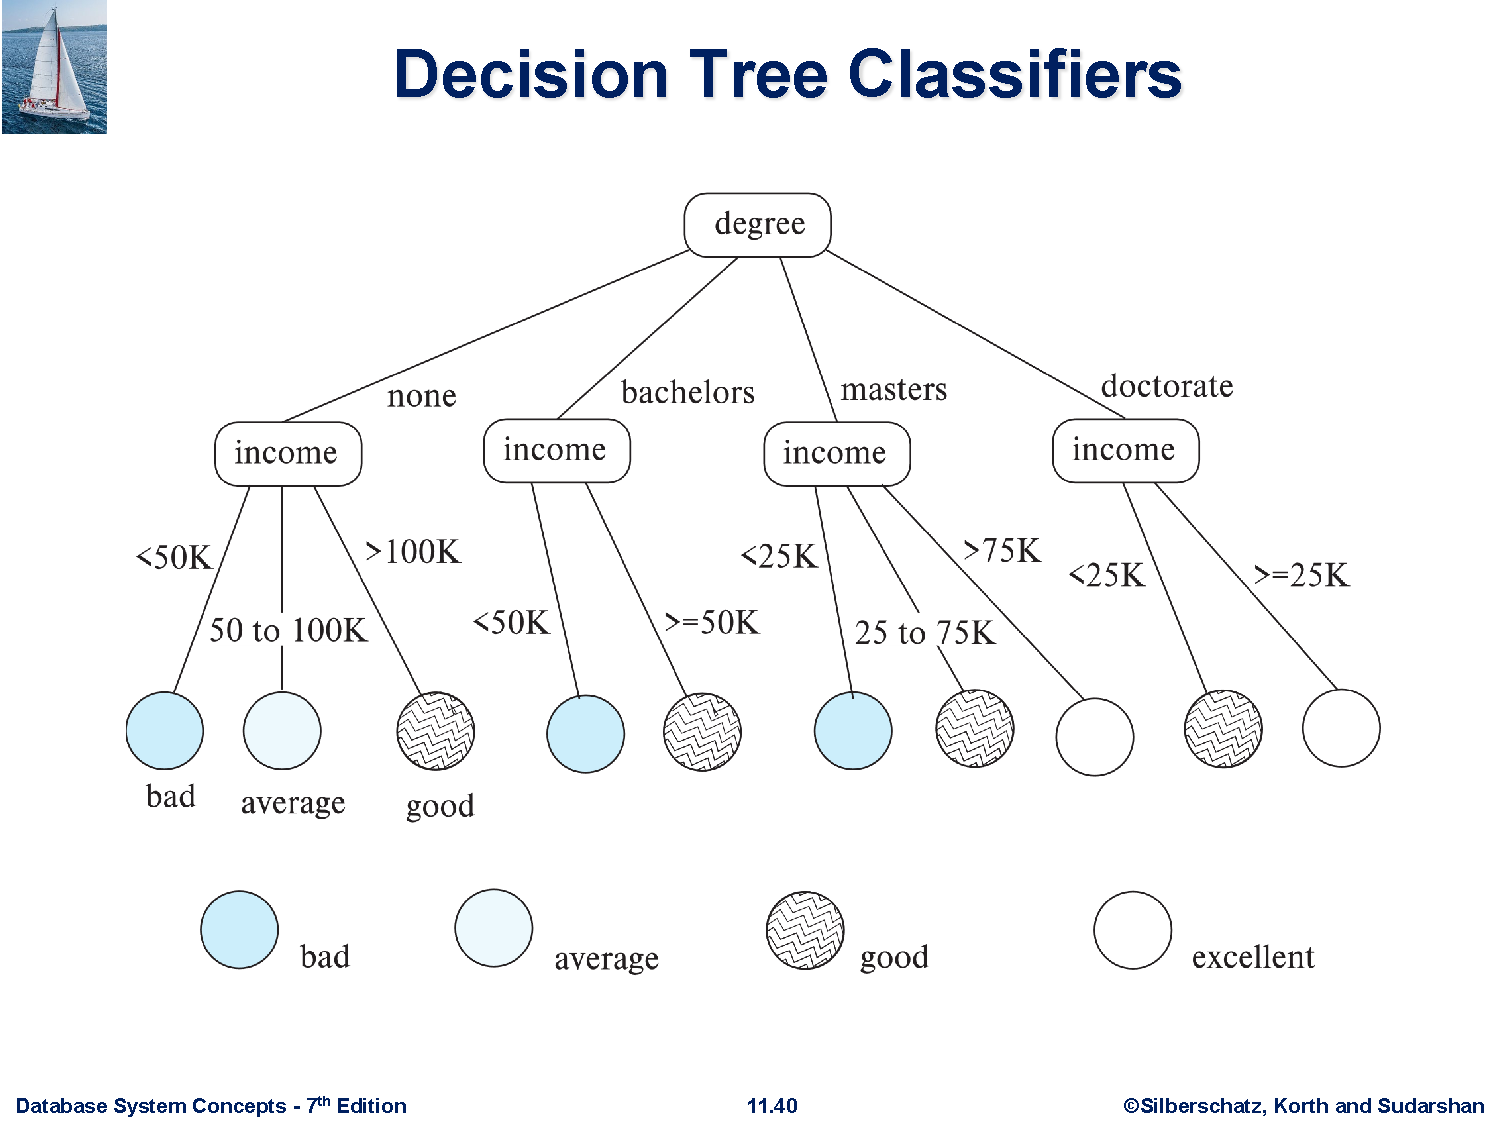
\includegraphics[width=\textwidth, trim={0cm 1cm 0cm 0cm}, clip]{slides/s39} }
\end{frame}
\begin{frame}{}
    \Wider{ 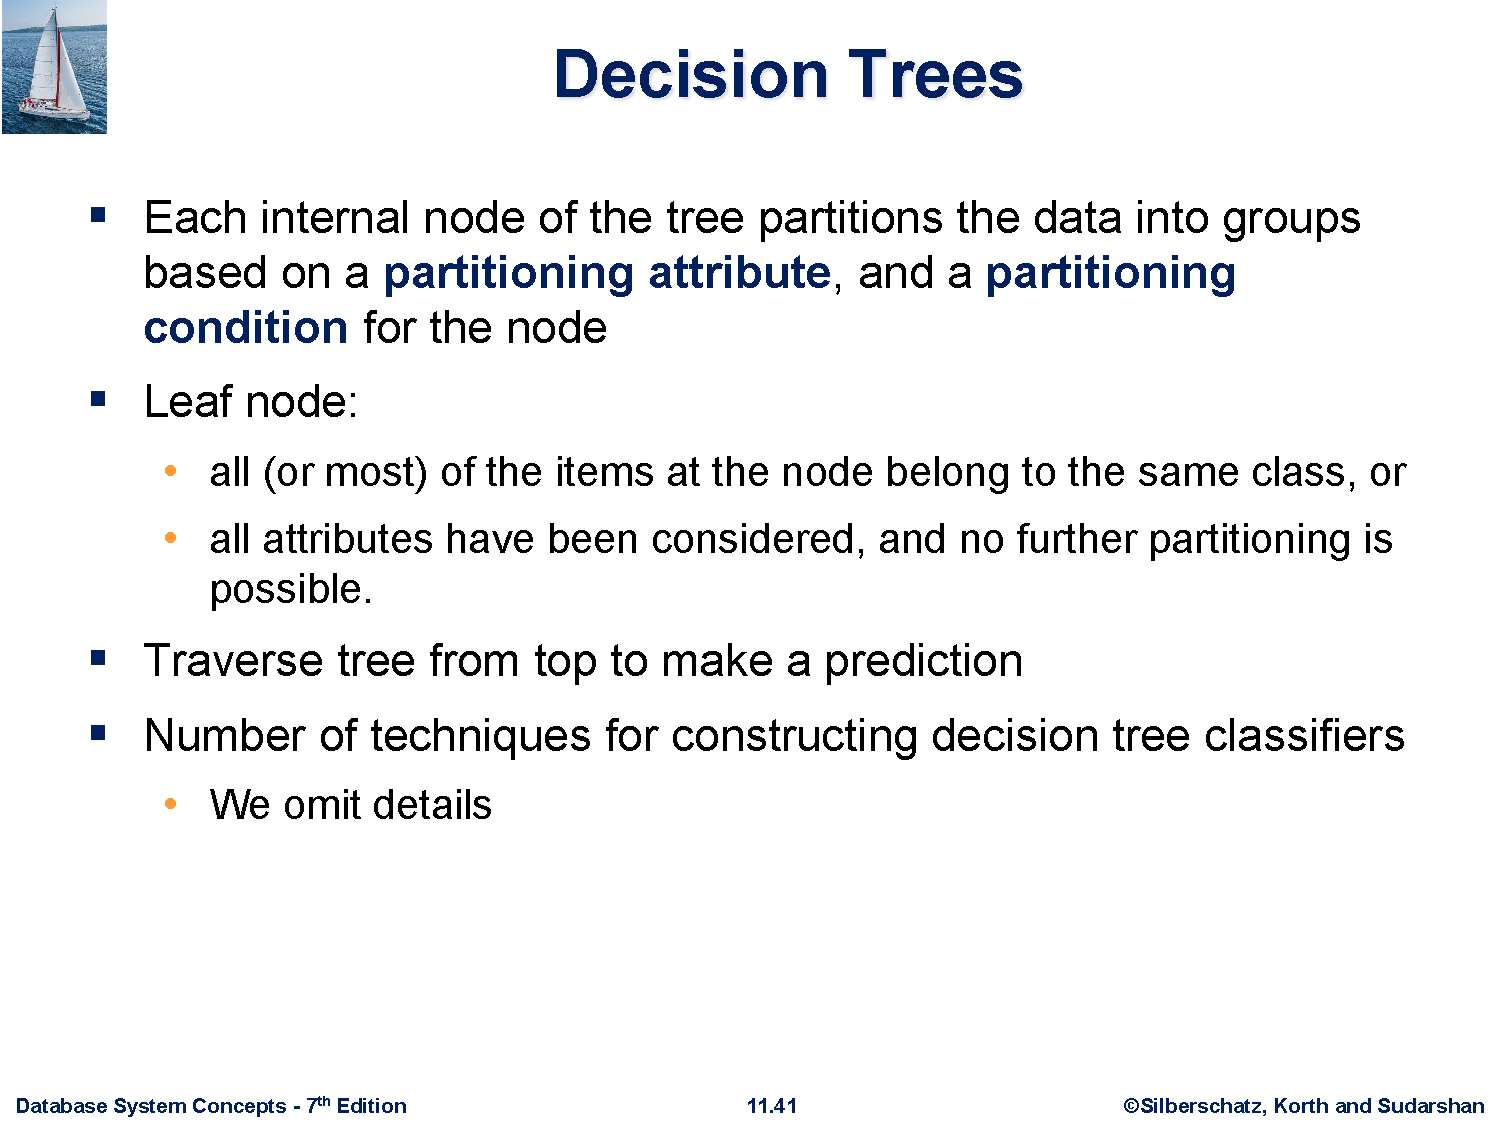
\includegraphics[width=\textwidth, trim={0cm 1cm 0cm 0cm}, clip]{slides/s40} }
\end{frame}
\begin{frame}{}
    \Wider{ 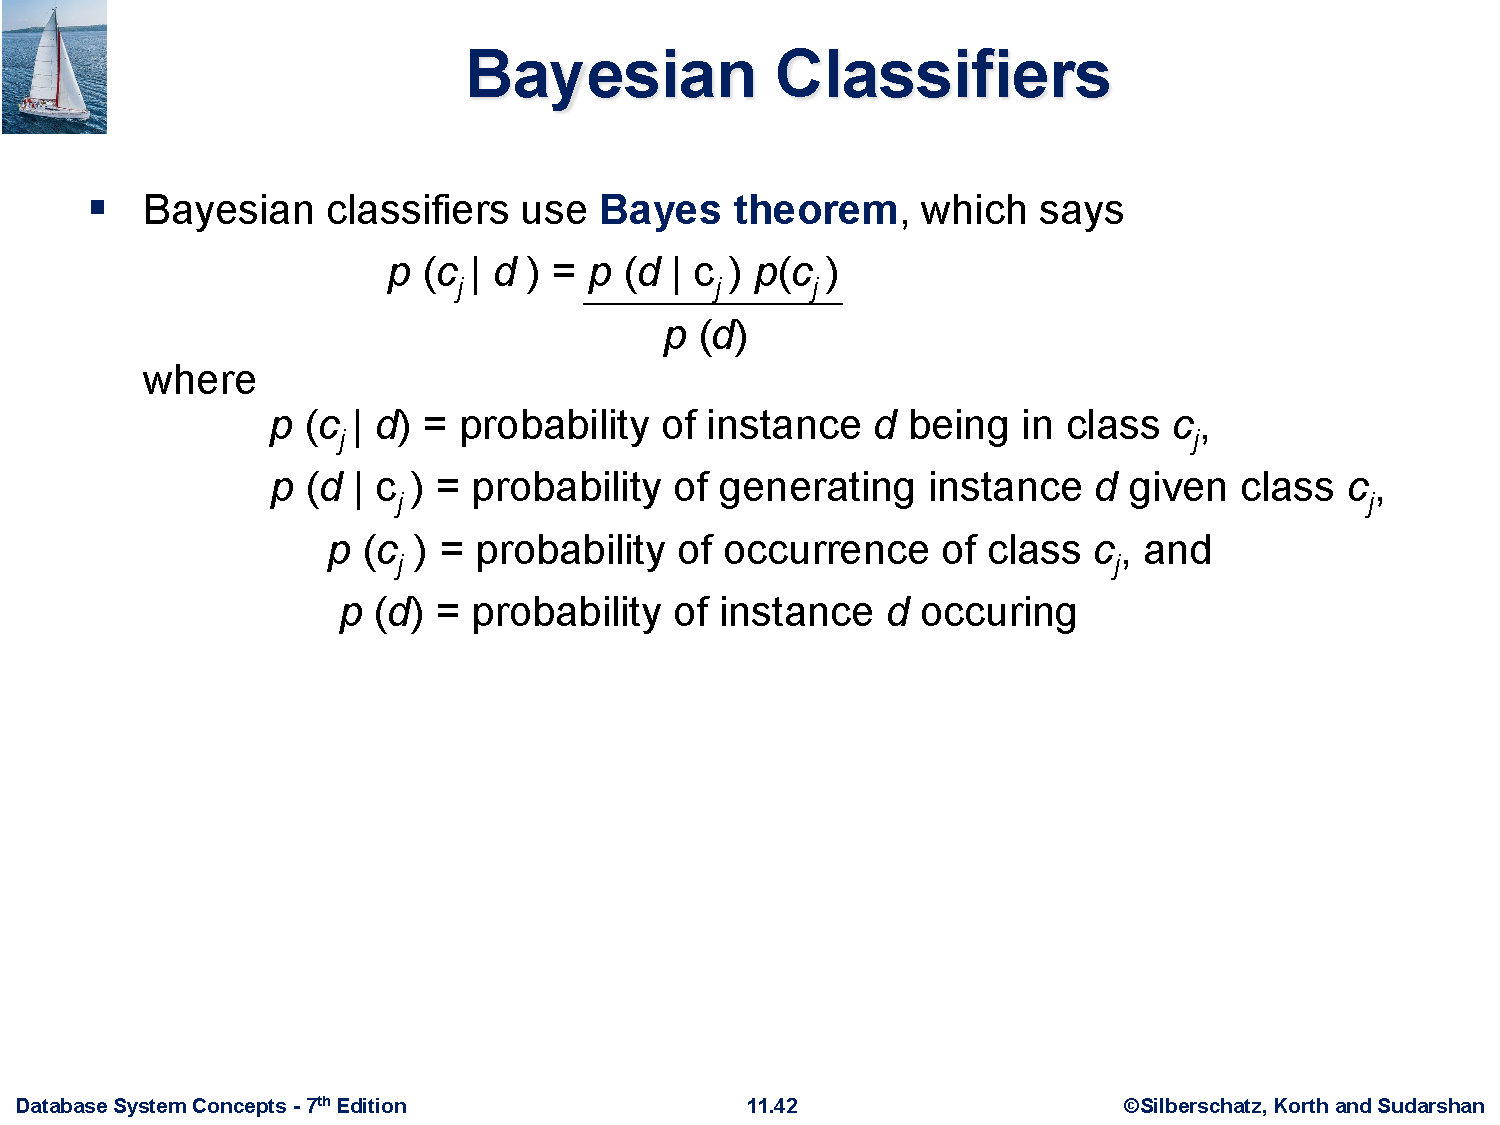
\includegraphics[width=\textwidth, trim={0cm 1cm 0cm 0cm}, clip]{slides/s41} }
\end{frame}
\begin{frame}{}
    \Wider{ 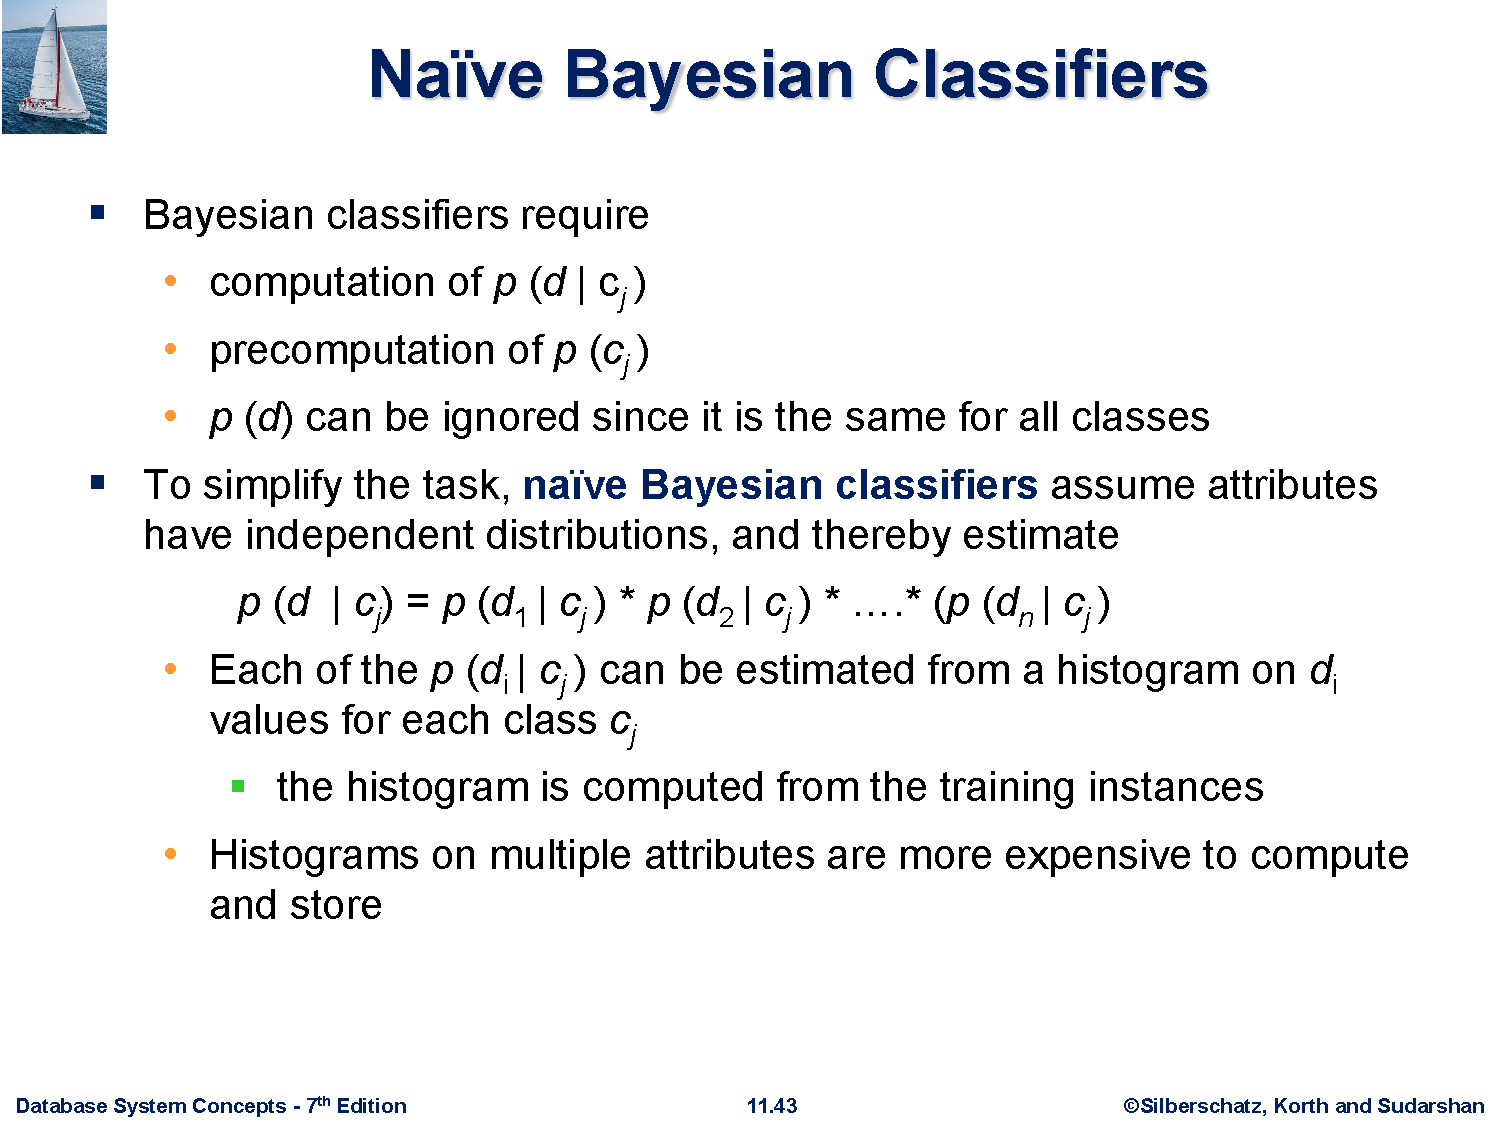
\includegraphics[width=\textwidth, trim={0cm 1cm 0cm 0cm}, clip]{slides/s42} }
\end{frame}
\begin{frame}{}
    \Wider{ 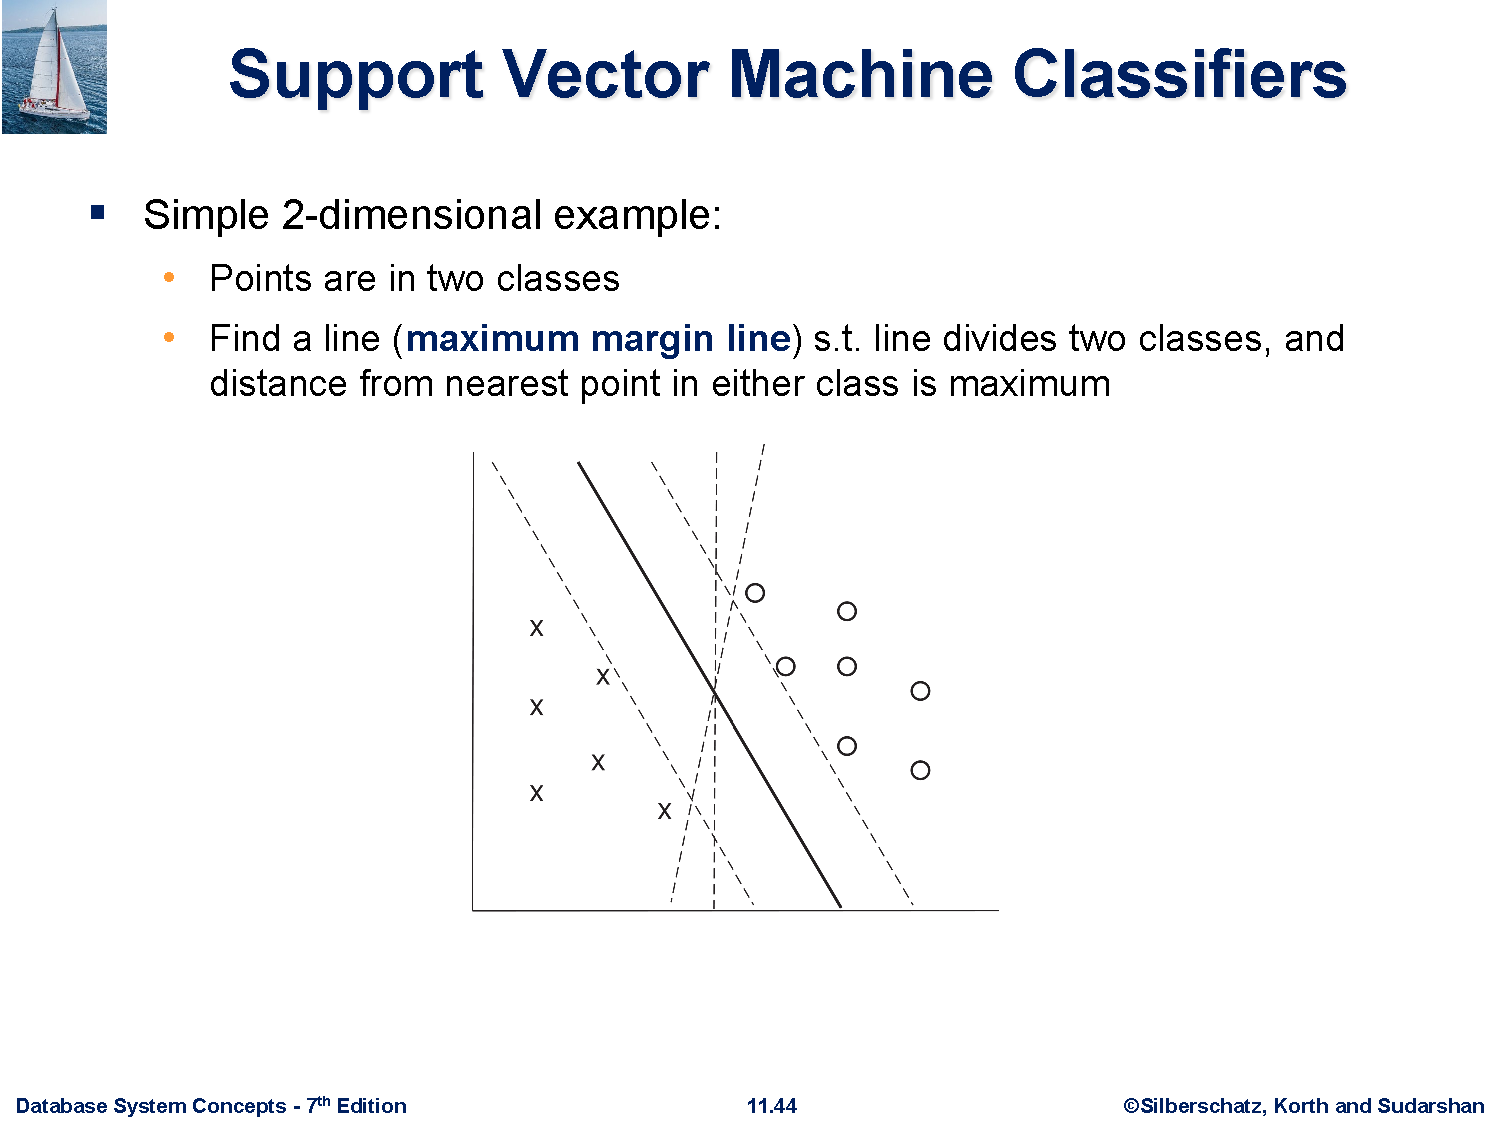
\includegraphics[width=\textwidth, trim={0cm 1cm 0cm 0cm}, clip]{slides/s43} }
\end{frame}
\begin{frame}{}
    \Wider{ 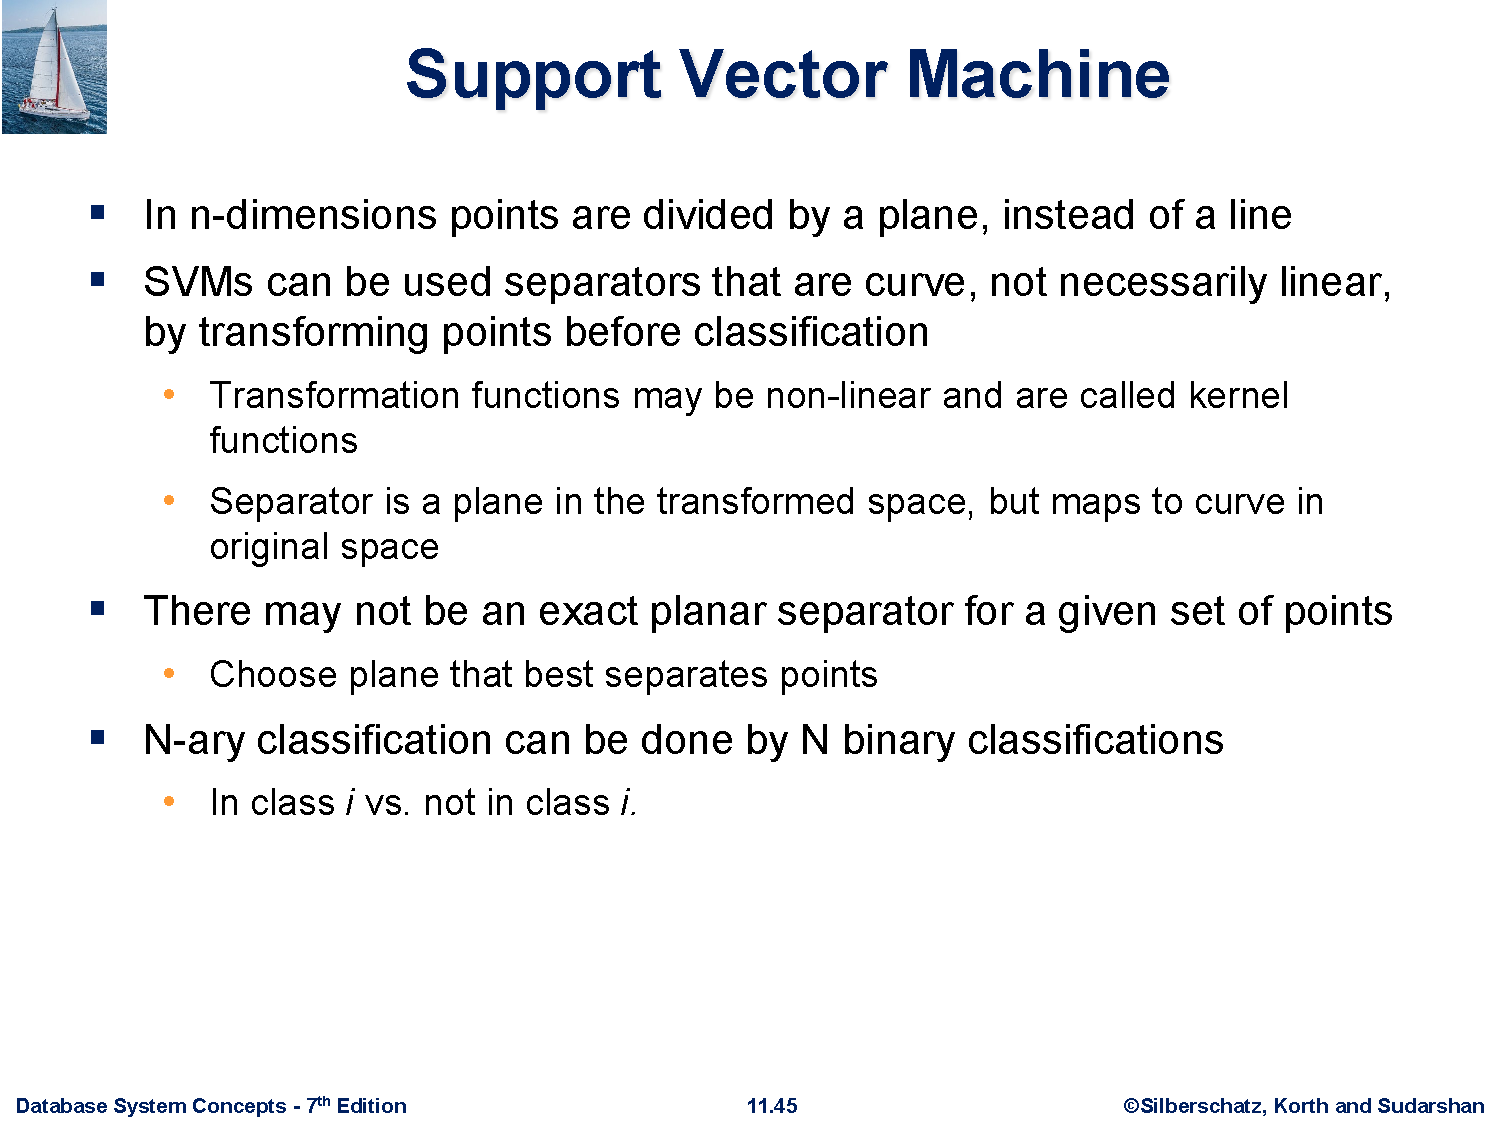
\includegraphics[width=\textwidth, trim={0cm 1cm 0cm 0cm}, clip]{slides/s44} }
\end{frame}
\begin{frame}{}
    \Wider{ 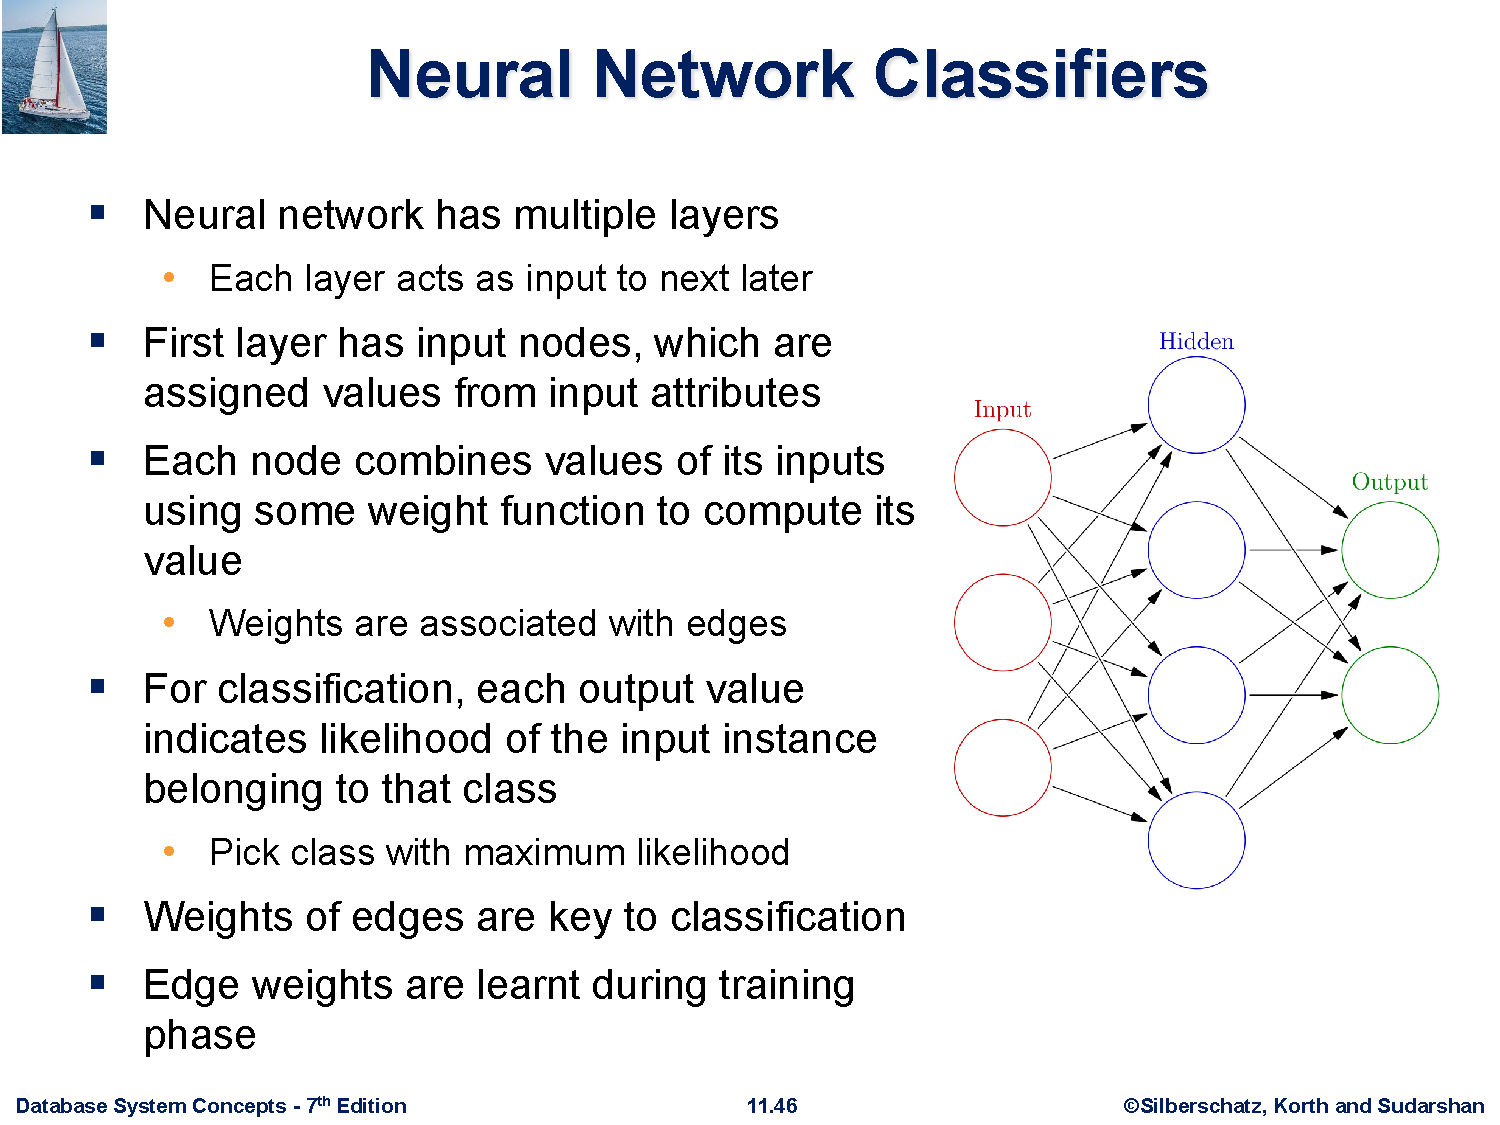
\includegraphics[width=\textwidth, trim={0cm 1cm 0cm 0cm}, clip]{slides/s45} }
\end{frame}
\begin{frame}{}
    \Wider{ 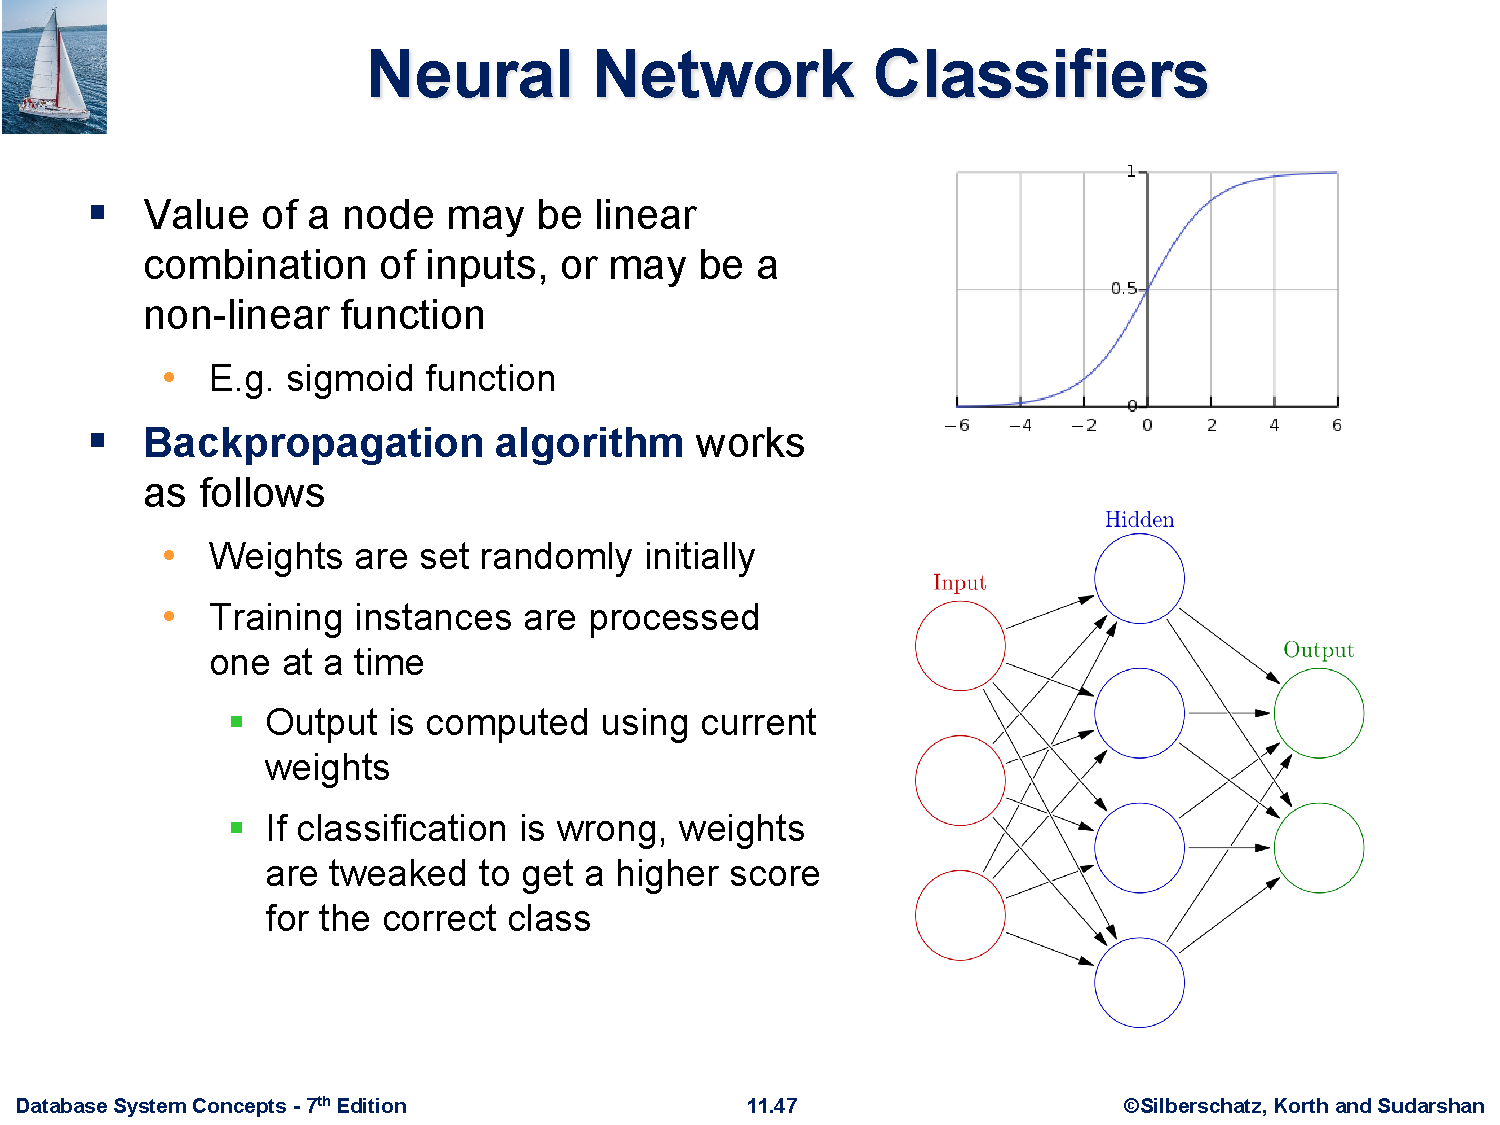
\includegraphics[width=\textwidth, trim={0cm 1cm 0cm 0cm}, clip]{slides/s46} }
\end{frame}
\begin{frame}{}
    \Wider{ 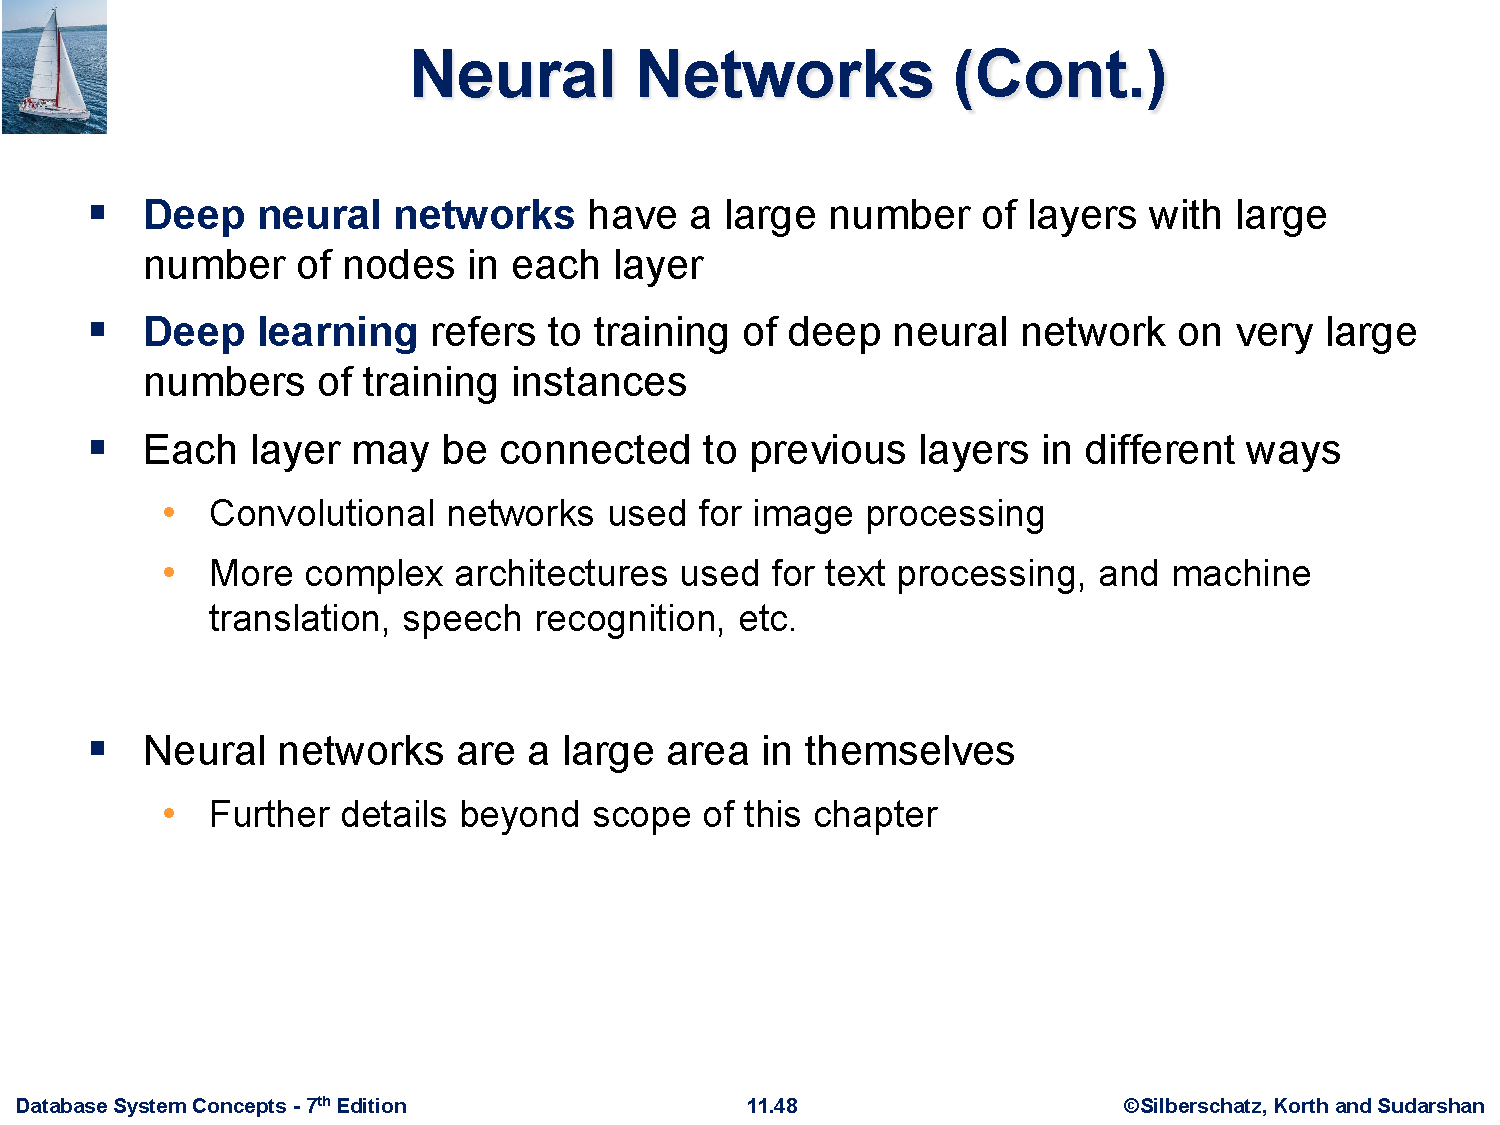
\includegraphics[width=\textwidth, trim={0cm 1cm 0cm 0cm}, clip]{slides/s47} }
\end{frame}
\begin{frame}{}
    \Wider{ 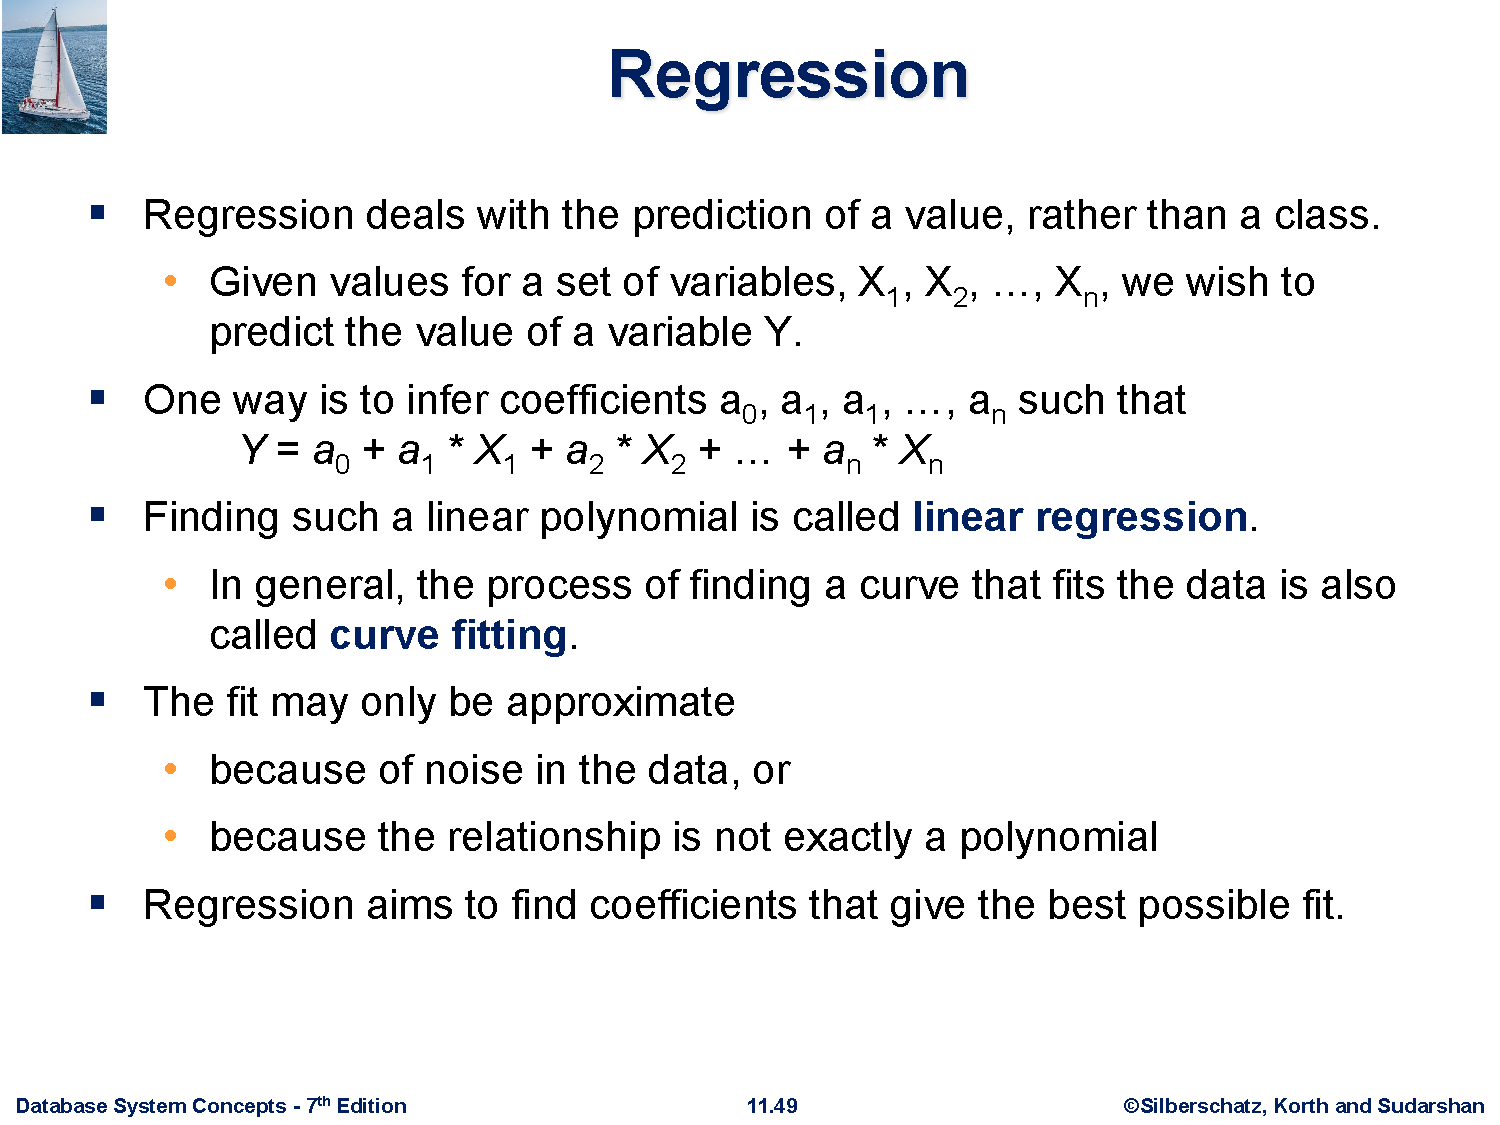
\includegraphics[width=\textwidth, trim={0cm 1cm 0cm 0cm}, clip]{slides/s48} }
\end{frame}
\begin{frame}{}
    \Wider{ 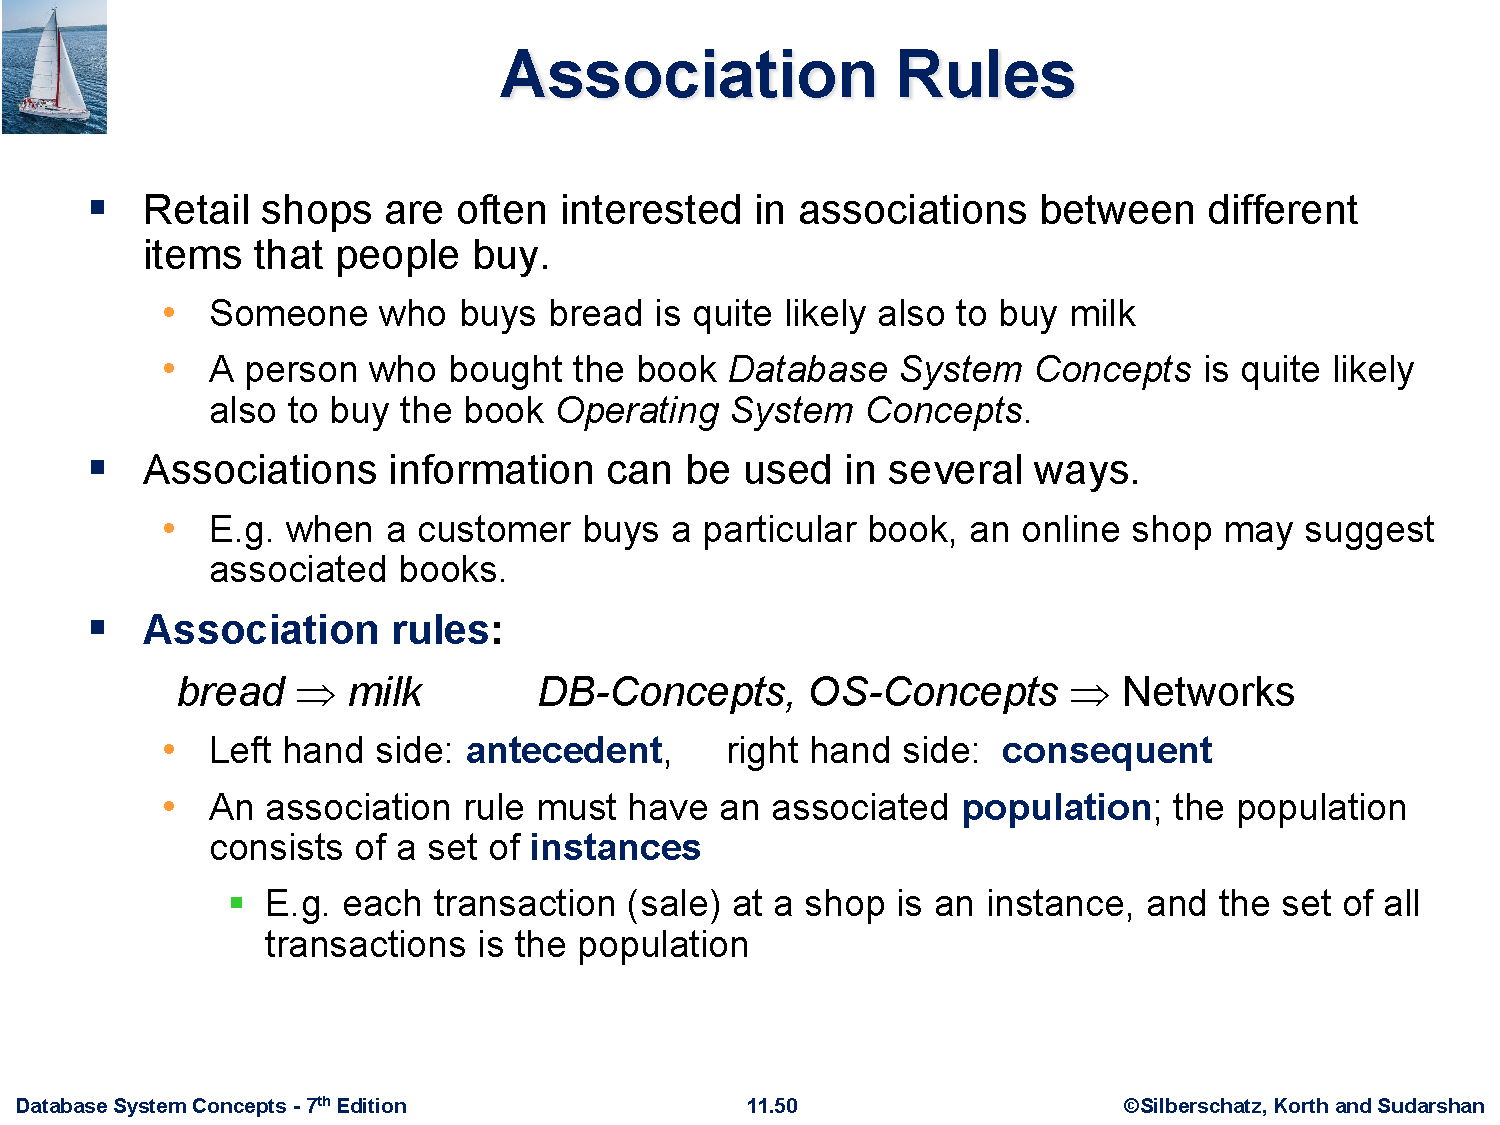
\includegraphics[width=\textwidth, trim={0cm 1cm 0cm 0cm}, clip]{slides/s49} }
\end{frame}
\begin{frame}{}
    \Wider{ 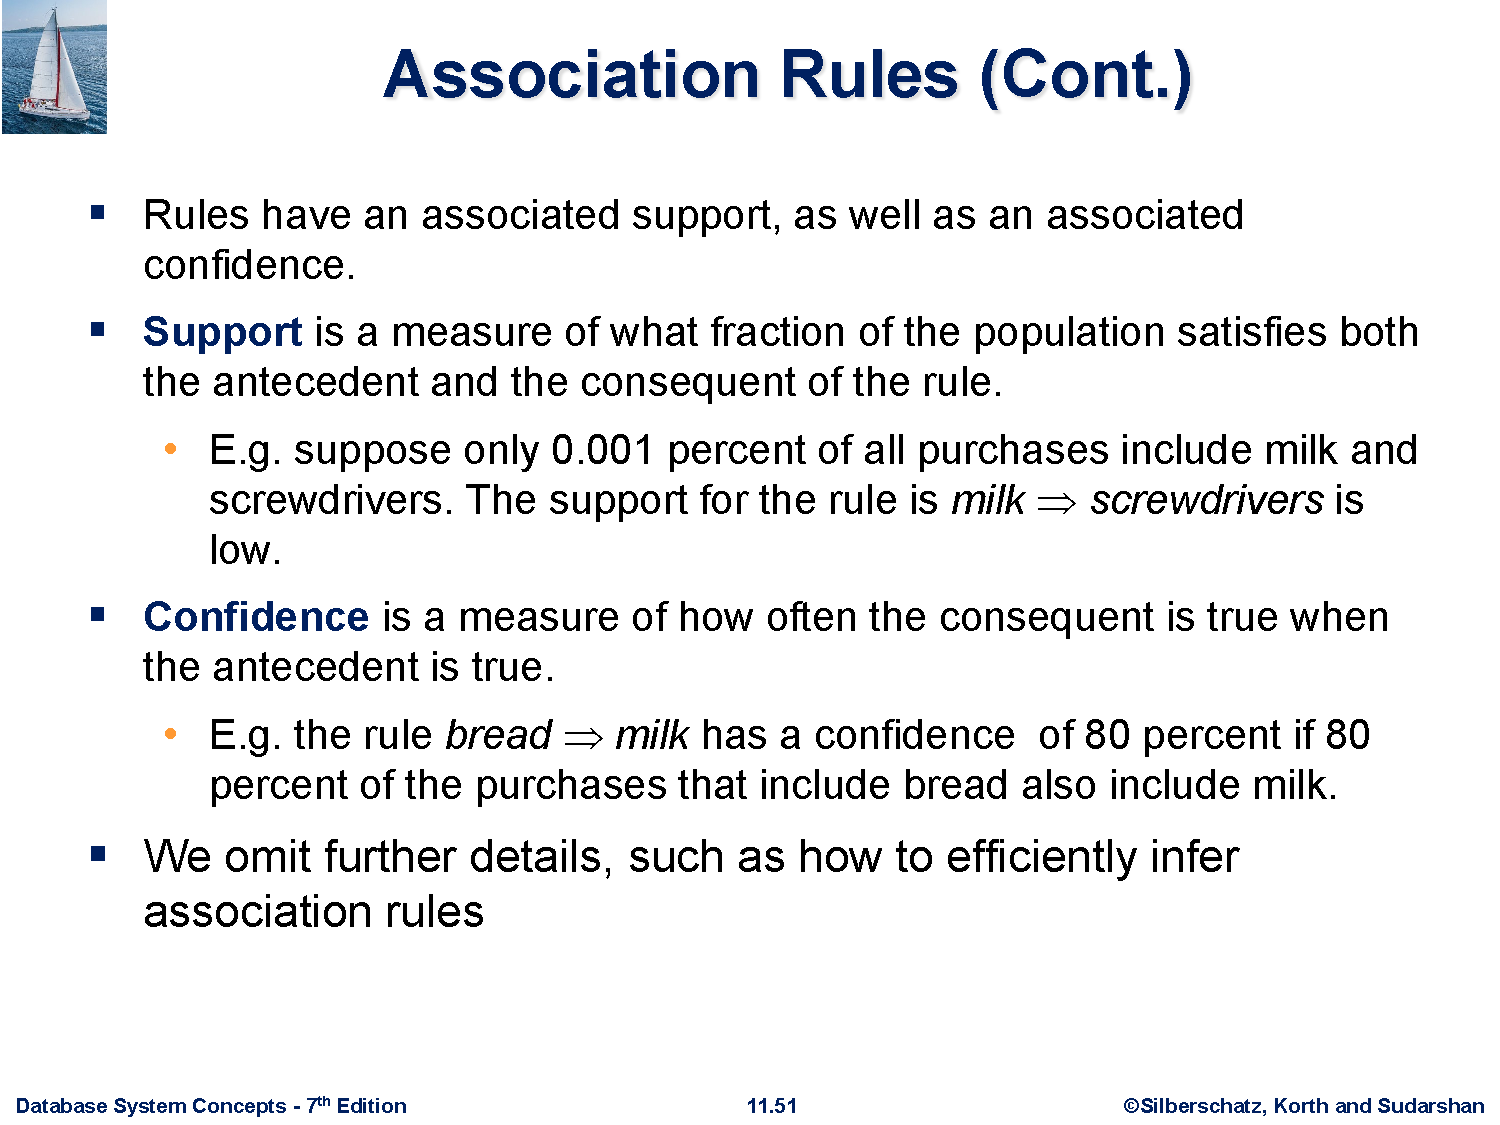
\includegraphics[width=\textwidth, trim={0cm 1cm 0cm 0cm}, clip]{slides/s50} }
\end{frame}
\begin{frame}{}
    \Wider{ 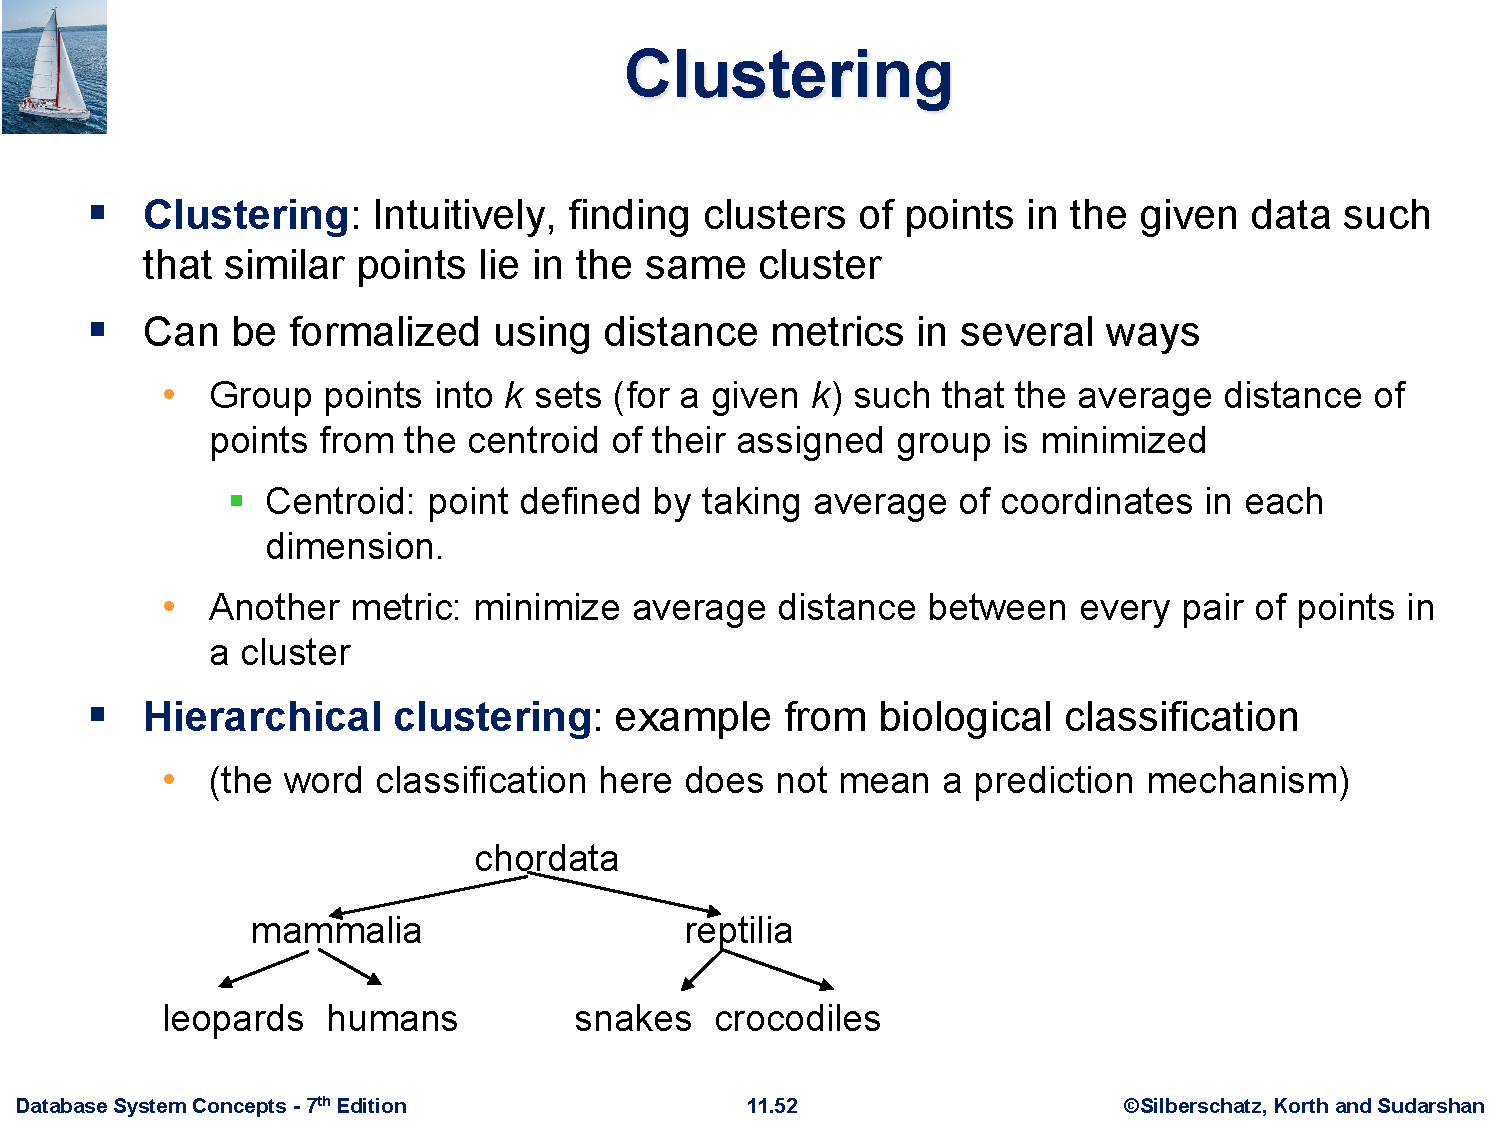
\includegraphics[width=\textwidth, trim={0cm 1cm 0cm 0cm}, clip]{slides/s51} }
\end{frame}
\begin{frame}{}
    \Wider{ 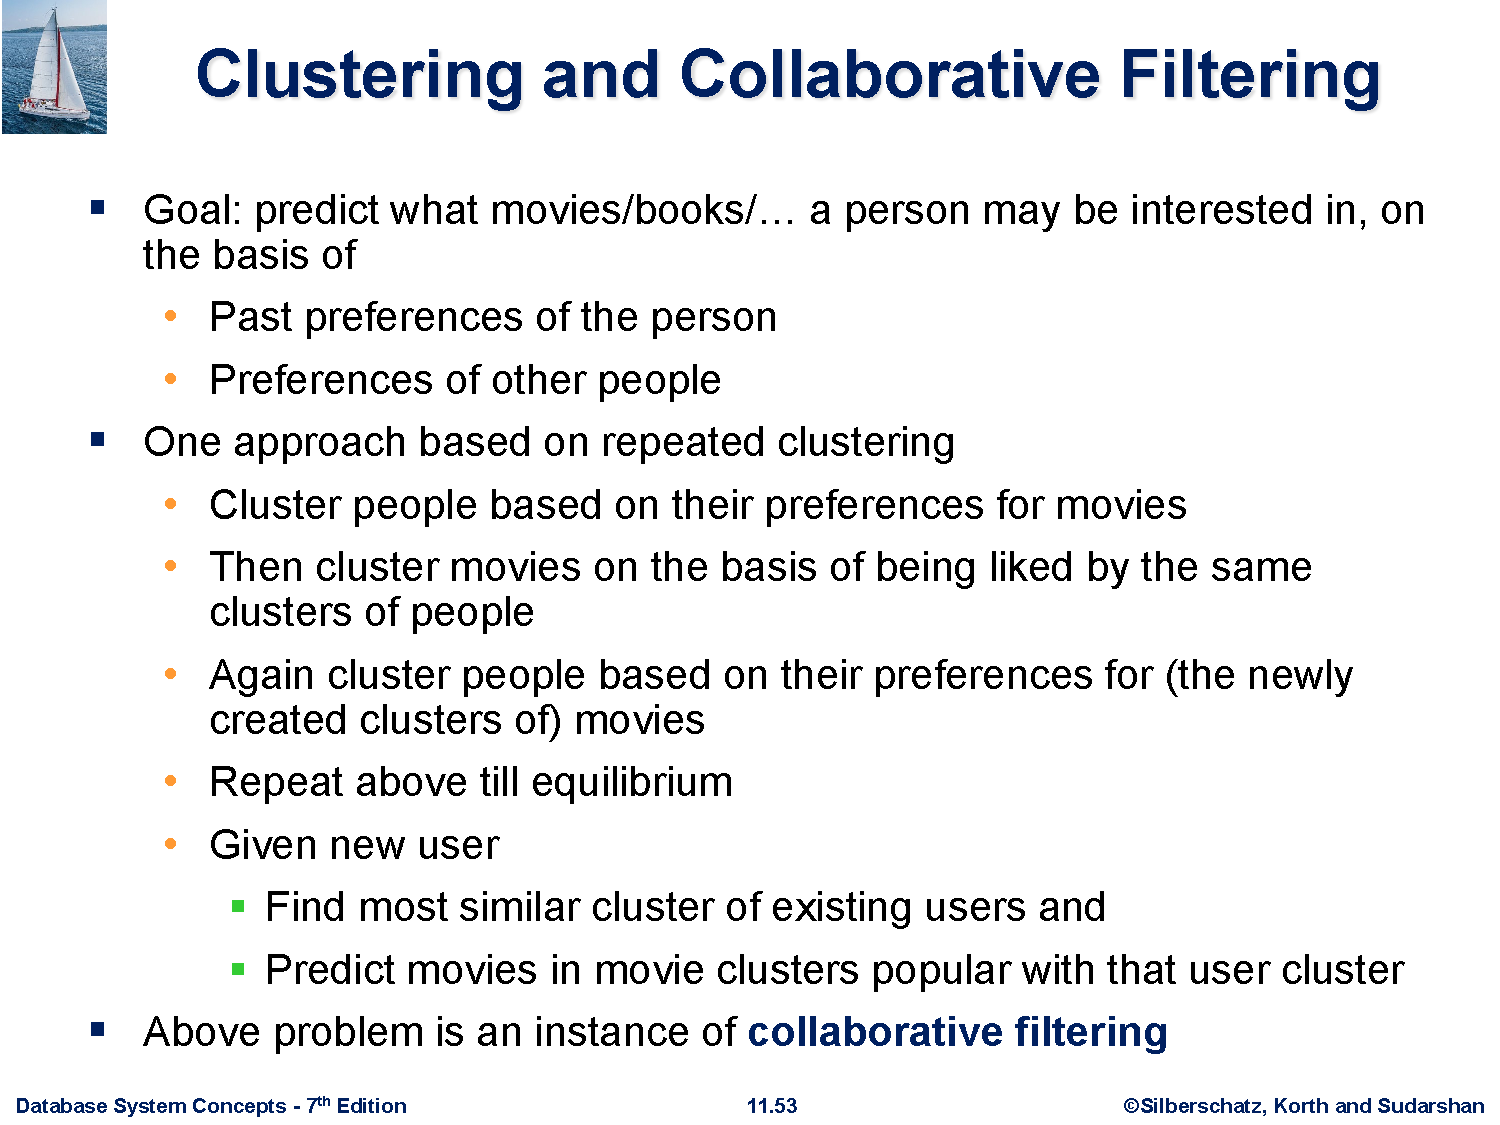
\includegraphics[width=\textwidth, trim={0cm 1cm 0cm 0cm}, clip]{slides/s52} }
\end{frame}
\begin{frame}{}
    \Wider{ 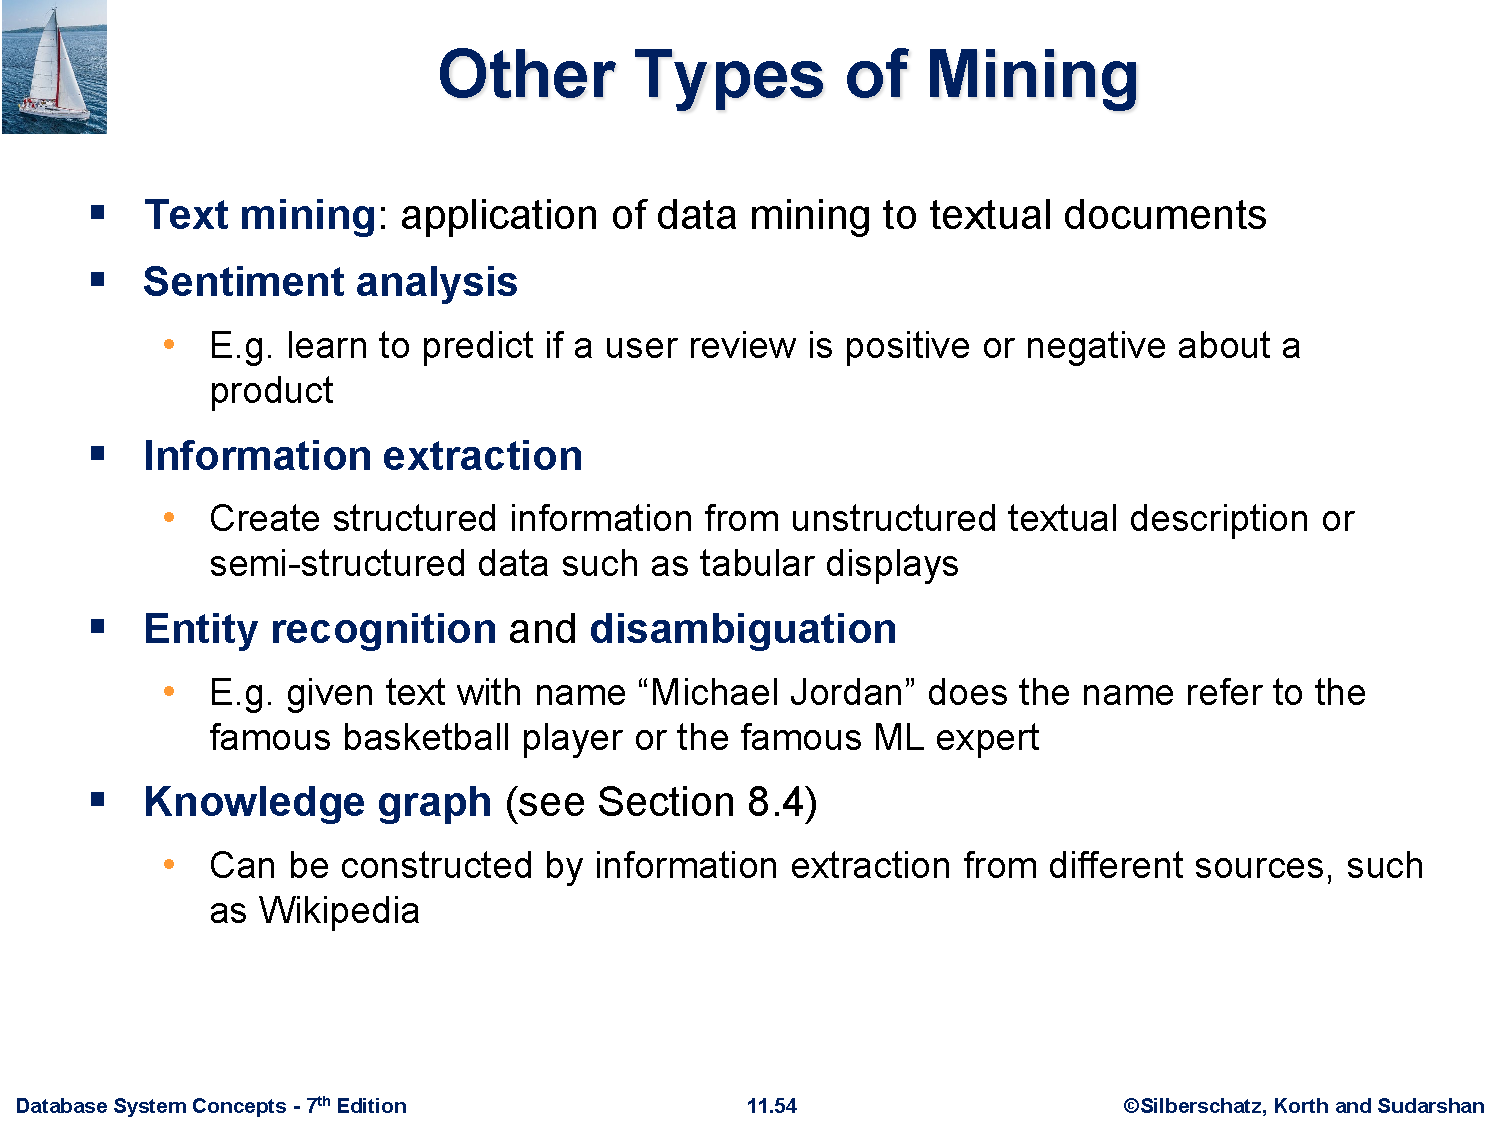
\includegraphics[width=\textwidth, trim={0cm 1cm 0cm 0cm}, clip]{slides/s53} }
\end{frame}

\begin{frame}{Database Administration: Data Analytics.}
    \centering
    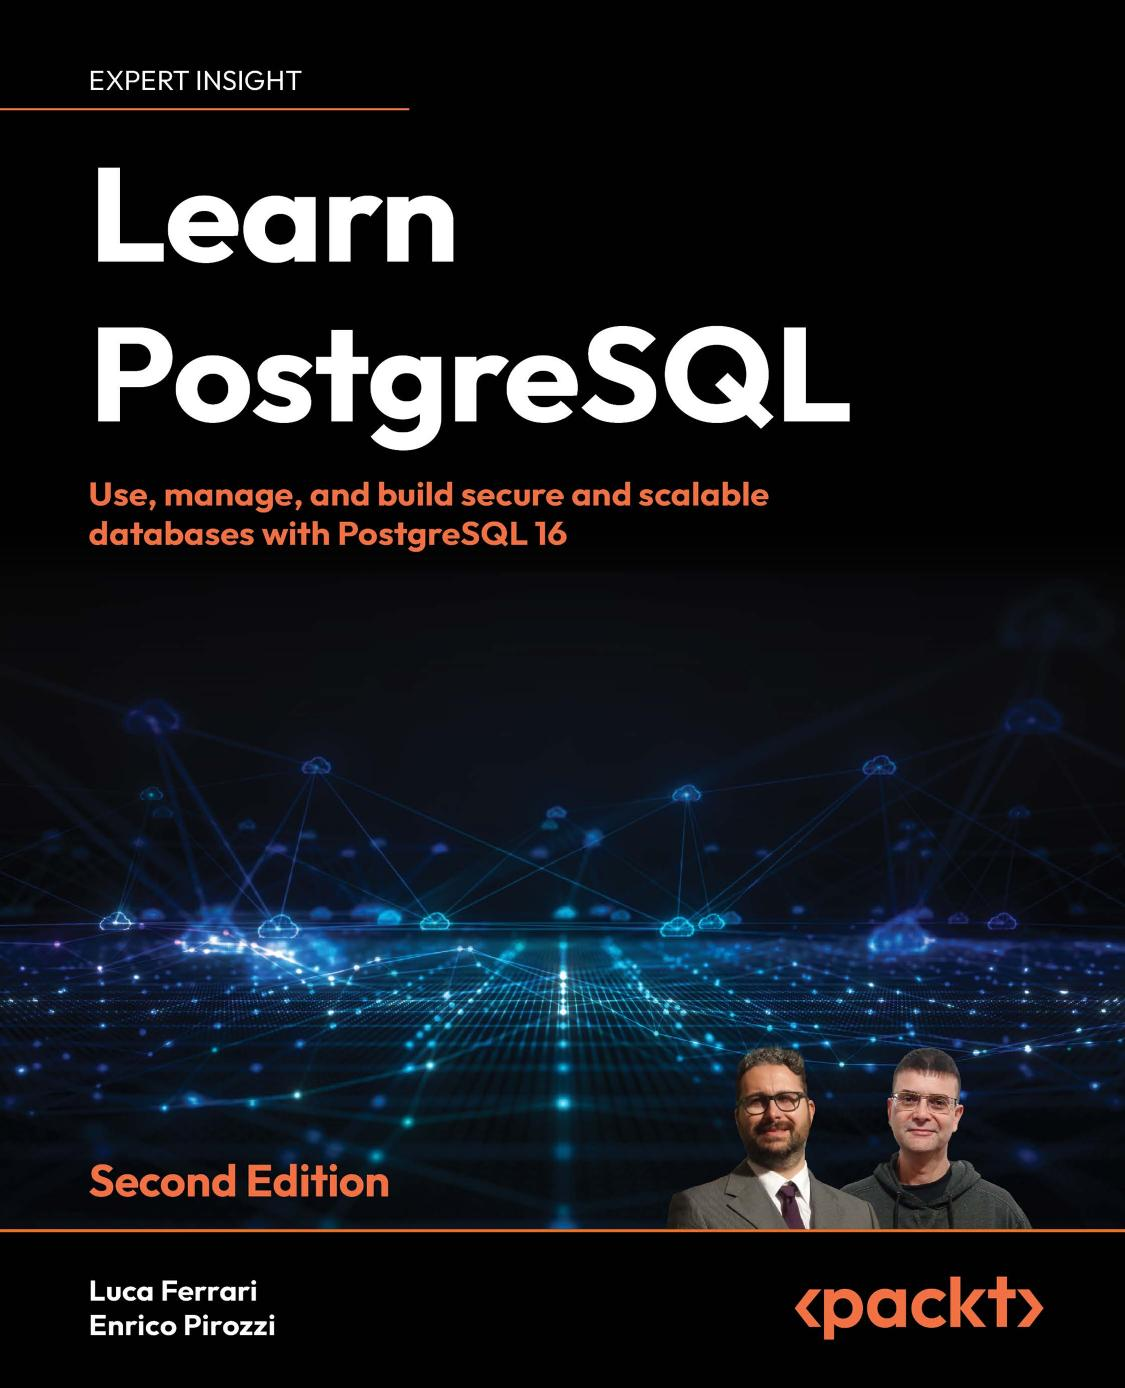
\includegraphics[width=0.4\textwidth]{figures/book_cover}\\
    \vspace{2mm}
    {
        \scriptsize
        Content has been extracted from \textit{Database System Concepts 7ed (Chapter 11)}, by Abraham Silberschatz, Henry Korth \& S. Sudarshan, 2019.  Visit \url{https://db-book.com/}.
    }
\end{frame}

\end{document}
